% !TEX program = pdflatex
% !BIB program = biber

%% One can optionally have all this inside a separate setup.tex
% !TEX program = pdflatex
% !BIB program = biber

% !TEX root = main.tex
\documentclass[10pt, a4paper]{report}
% \documentclass[12pt, a4paper, oneside]{memoir}
% \chapterstyle{veelo}

%% Sets page size and margins
\usepackage[a4paper,top=3cm,bottom=2cm,left=3cm,right=3cm,marginparwidth=1.75cm]{geometry}
%\usepackage[left=2cm,top=2cm,bottom=2cm,bindingoffset=1cm]{geometry}

\usepackage[utf8x]{inputenc}
\usepackage{graphicx}
\usepackage{float}
\usepackage{imakeidx}
\usepackage{amsmath}
\usepackage[colorlinks=true, allcolors=blue]{hyperref}
\usepackage{graphicx}
\usepackage{float}
\usepackage{imakeidx}
\usepackage{amsmath}
\usepackage{url}
\usepackage[export]{adjustbox}
\usepackage{subcaption}
\usepackage[toc,page]{appendix}

%% Useful packages
\usepackage[colorinlistoftodos]{todonotes}
\usepackage[T1]{fontenc}

%% Language and font encodings
\usepackage[english]{babel}

%% Define a few colours to be used throughout the document
\usepackage{tikz,xcolor}
\definecolor{TextColor}{HTML}{000000}
\definecolor{SideColorDark}{HTML}{000000}
\definecolor{MainColor}{HTML}{0000FF}
\definecolor{OppositeColor}{HTML}{FF0000}
\definecolor{HighlightColor}{HTML}{FFFF00}


%% Code block style
%  Load the \ttfamily font
\usepackage[T1]{fontenc}
\usepackage[scaled]{beramono}

%  Format code blocks
\usepackage{listings}
%  Change caption name
\renewcommand*{\lstlistingname}{Code block}
\captionsetup[lstlisting]{margin=0cm,format=hang,font=small,format=plain,labelfont={bf,up},textfont={it}}
%  Style
\lstset{
  showstringspaces=false,
  formfeed=\newpage,
  commentstyle=\itshape,
  backgroundcolor=\color{gray!5},
  breakatwhitespace=false,         % sets if automatic breaks should only happen at whitespace
  breaklines=true,                 % sets automatic line breaking
  captionpos=b,                    % sets the caption-position to bottom
  commentstyle=\color{gray},    % comment style
  escapeinside={\%*}{*)},          % if you want to add LaTeX within your code
  keepspaces=true,
  numbersep=2mm,                   % how far the line-numbers are from the code
  showspaces=false,
  showstringspaces=false,
  showtabs=false,
  stepnumber=1, numberfirstline=false,
  basicstyle=\linespread{1}\footnotesize\ttfamily,
  keywordstyle=\bfseries\color{MainColor},
  stringstyle=\itshape\color{OppositeColor},
  numberstyle=\footnotesize\ttfamily\color{gray},
  numbers=left,xleftmargin=4mm,framexleftmargin=0mm,xrightmargin=0mm,
  frame=top,frame=bottom,
}

\title{Insert title here}
\author{Daniel Robinson\\18361137}

\pagenumbering{roman}
\setlength\parindent{0pt}

\begin{document}
% \maketitle
    \begin{titlepage}
        \begin{center}
            \vspace*{1cm}
            
            \begin{figure}
			\centering
            
\includegraphics[scale=2]{images/UScrest-top.jpg}
            \end{figure}
            
            \huge
            \textbf{Normalized Differential Vegetation Index Mapping}

            \large            
            \vspace{2.5cm}

            \textbf{Daniel Robinson\\18361137}

            \vspace{2.5cm}    
            
            \textbf{Report submitted in partial fulfilment of the requirements of the module Project (E) 448
            for the degree Baccalaureus in Engineering in the Department of Electrical and Electronic
            Engineering at the University of Stellenbosch}
            
            \vspace{4cm} 
            
            \textbf{STUDY LEADER: Corné van Daalen\\DATE: November 2017}
            
            
        \end{center}
\end{titlepage}

\setcounter{secnumdepth}{-2}% default for "report" is 2

\newpage
\chapter{Declaration of own work}

I, the undersigned, hereby declare that the work contained in this report is my own original work
unless indicated otherwise.

\vspace{2.5cm}   

Signature: \hrulefill

\hspace*{0mm}\phantom{Signature: }Daniel Robinson

\hspace*{0mm}\phantom{Signature: }BEng Electrical \& Electronic

\vspace{1cm}   

Date:\space\space\space\space\space\hrulefill

\chapter{Abstract}

This report presents the design and analysis necessary for an autonomous system to acquire beneficial agricultural data within a desired environment. Various implementations are compared, before a novel design is presented. An aerial drone is designed and built using predominantly local supplies. Images are acquired and processed.\\

\noindent
(Still to be expanded on).

\chapter{Uitreksel}

(Still to be expanded on).

\chapter{Acknowledgements}

I would like to thank the following people for their support:
\begin{itemize}
    \item Louw Hopley, for giving birth to the idea.
    \item Alan Knott-Craig, for introducing me to Chris Antoniesson, for we went on a flight test together which returned very useful data.
    \item My family, who have been amused and for their unwavering love and support.
    \item Dr C van Daalen, for his guidance and support throughout the course of this project.
\end{itemize}

%\frontmatter
\cleardoublepage
\tableofcontents

\clearpage
\label{listoffigures}
\addcontentsline{toc}{chapter}{\listfigurename}
\listoffigures

\clearpage
\addcontentsline{toc}{chapter}{\listtablename}
\label{listoftables}
\listoftables

\chapter{List of Symbols}
\begin{table}[H]
\centering
\begin{tabular}{l|r|r}
Symbol & Description & Units\\\hline\\
$F$ & Fundamenal Matrix & 3x3\\
$R$ & Rotation Matrix & 3x3\\
$T$ & Translation Matrix & 3x3\\
\end{tabular}
\caption{\label{tab:symb}Table depicting list of symbols. (Will probably not have this caption)}
\end{table}

\chapter{List of Abbreviations}
\begin{table}[H]
\centering
\begin{tabular}{l|r}
Abbreviation & Description \\\hline
UAV & Unmanned Aerial Vehicle \\
NDVI & Normalised Differential Vegetation Index\\
IR & Infra Red\\
PAR & Photosynthetically Active Radiation\\
PCB & Printed Circuit Board\\
CSI & Camera Serial Interface\\
SBUS & Serial Bus ?\\
GPIO & General Purpose In Out\\
\end{tabular}
\caption{\label{tab:abbr}Table depicting list of abbreviations. (Will probably not have this caption)}
\end{table}

\chapter{Matrix Notation}

(Still to be expanded on).

\setcounter{secnumdepth}{2}

\chapter{Introduction}

\pagenumbering{arabic}

There is currently a water shortage crisis in South Africa, as well as in other parts of the world, potentially due to global warming. One of the sectors that it affects is agriculture. The water shortage puts added stress on farmers who are effectively aiming for the greatest yield. Factors that lower yield quality include non-uniform distribution of water, fertilizer, pesticides and undetected plant disease.\\

To mitigate such problems, farmers would typically use their expertise in observation from the ground. It can be a time consuming task, especially over areas of a few square kilometres. If ground-based sensor data is used, the readings may be too sparse due to the cost and complexity of multiple static sensors, and even more so for hand-held readings. Perhaps a simpler, large-scale method of observing such changes at once can be used.

\section{Purpose of the project}

The purpose of the project is to investigate infra-red mapping of vegetation, which can thus potentially determine the impact of human and environmental factors such as diseases, erosion, variances in fertiliser and water application.\\

If the data can be beneficial to farmers, and more cost-effectively, then it can be seen that the project is a success.

\section{Problem Statement}\

In brief, the problem addressed in the project is to develop a nadir\footnote{Downwards facing} infra-red observation platform to map agricultural areas from height.\\

A popular algorithm for analysis is the normalized differential vegetation index, or NDVI for short. This particular one will be the focus of the project. If successful, it opens up the possibility of investigating other useful indices, perhaps even for the mining industry.\\

Cameras will be used to acquire data. Filters, using colour subtraction, will be used to isolate parts of the spectrum required by the vegetation index.\\

To monitor large areas in a short period of time, one can use satellites or vehicles such as airstats, planes, hot air balloons and helicopters. The vehicles can be classified into manned and unmanned aerial vehicles. UAVs have significantly less safety precautions, regulations, cost, and are less subject to wear and tear, meaning more flights (cite).\\


The implementation of autonomous systems can be costly. It also depends on what type of UAV is used. Unmanned aeroplanes  are fast and can cover vast areas. With enough height, the effects of motion blur in imagery tend to zero. On the other hand, they are significantly complex to operate, and although it would be ambitious, it would be impractical for a project such as this. Aerostats\footnote{Lighter than air aircraft that gains its lift through the use of a buoyant gas} and hot air balloons\footnote{Unpowered aerostat which has no means of propulsion and is usually tethered} can stay up for long periods of time, but are impractical due to the limited uses, and difficulty in moving such a vehicle once in the air. Drones have a price point between aeroplanes and hot air balloons, but they can take accurate and versatile high resolution images, with less risk to the camera equipment than a plane.\\

Thus, a drone is designed and built to demonstrate proof of concept of a more cost effective model compared to other drone solutions that exist in the market today.\\

For this project, it is assumed that NDVIs are calculated predominantly in the farming sector, and that the values will be relatively stable when affected by sunlight, cloud cover and other factors.

\section{System Overview}

Figure \ref{fig:scenario} illustrates a typical scenario where the system is used.\\

\begin{figure}[H]
\centering
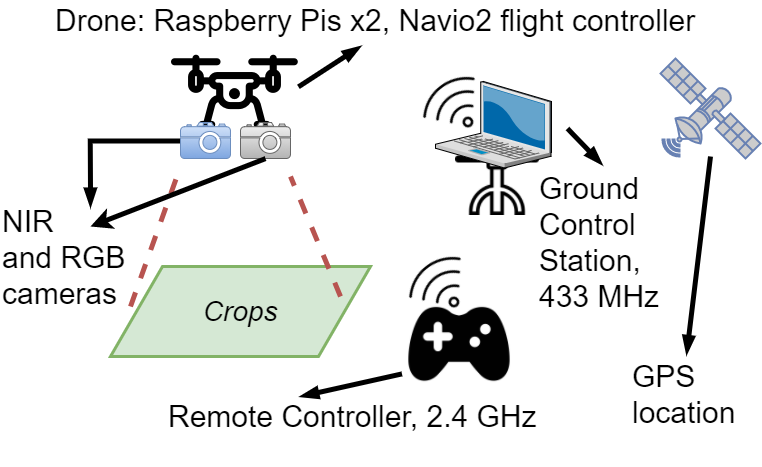
\includegraphics[scale=0.4]{images/drone_ndvi_scenario.png}
\caption{Illustration of the system as an overview}
\label{fig:scenario}
\end{figure}

A farmer would utilize the equipment for the purposes of capturing data. Specifically, the cameras on the drone will capture information about the farmer's crops, the remote controller is a failsafe to take over from autopilot, the GPS location georeferences each photo for the purpose of mapping, and the ground control station doubles as a mission planner and for the use of direct post-processing.\\

An example NDVI result is shown in Figure \ref{fig:vineyard_leaves}. Notice the different effects of the sun and shadows on the leaves.

\begin{figure}[H]
\begin{subfigure}{0.5\textwidth}
\centering
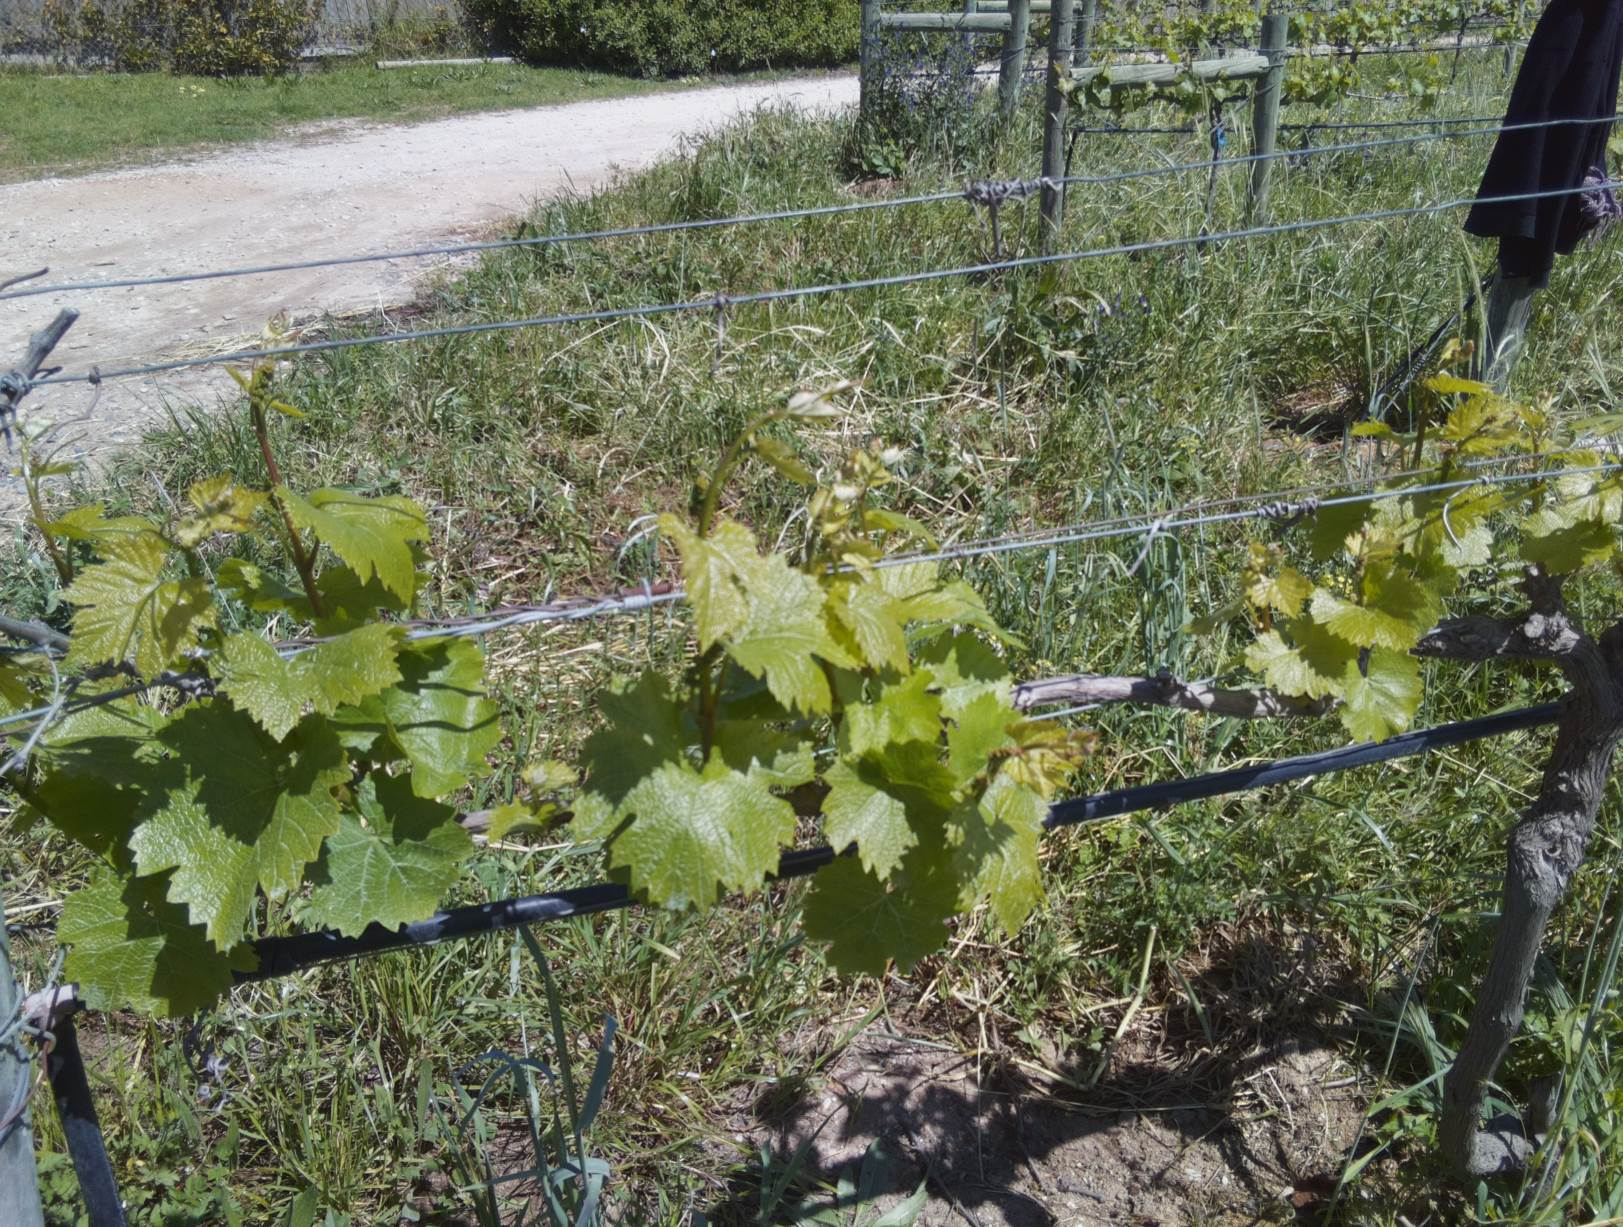
\includegraphics[scale=0.17]{images/rgb_leaves.jpg}
\caption{RGB image}
\end{subfigure}
\begin{subfigure}{0.5\textwidth}
\centering
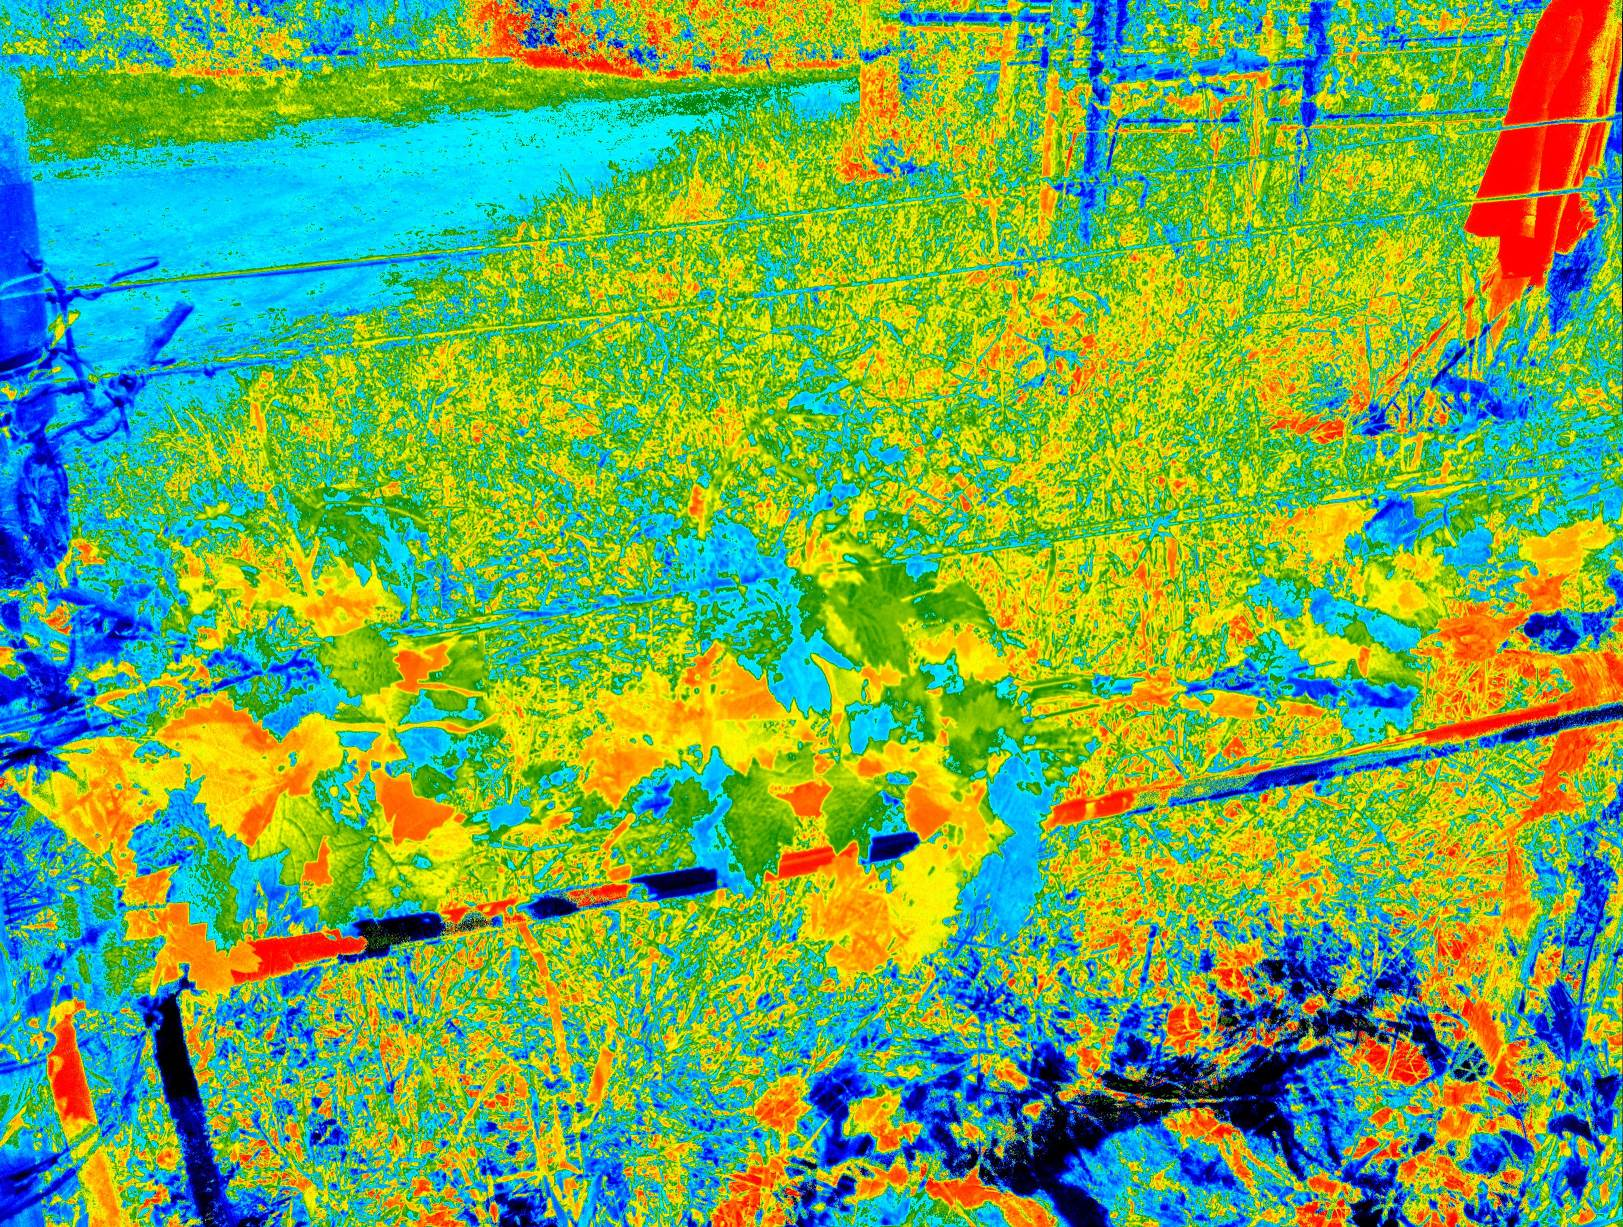
\includegraphics[scale=0.17]{images/ndvi_leaves.jpg}
\caption{Processed NDVI image}
\end{subfigure}
\caption{Closeup of vineyard leaves}
\label{fig:vineyard_leaves}
\end{figure}

%An implementation process of the system is illustrated in Figure \ref{fig:overview}. These processes will be expanded on and explained in the relevant chapters.
%
%\begin{figure}[H]
%\centering
%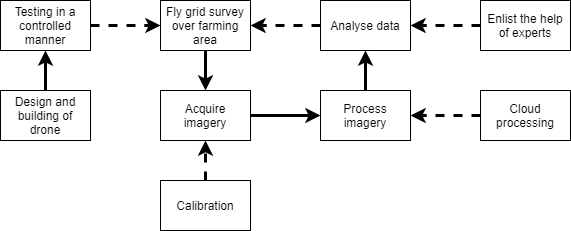
\includegraphics[scale=0.6]{images/thesis_overview.png}
%\caption{Implementation process}
%\label{fig:overview}
%\end{figure}
%
%Various drones, cameras, filters and processing techniques will be presented, as well as optimal choices depending on available resources.\\

A literature study will be investigated in Chapter 2, with drone design and construction in Chapter 3. Image acquisition and calibration will be handled in Chapter 4, and image processing in Chapter 5. Lastly, system integration and testing will be discussed in Chapter 6.
\label{chapter:intro}
\chapter{System Architecture}

The system architecture defines the system components, interrelationships and fundamental concepts to note.

\section{Infrared light}

Infrared light extends from the nominal red edge of the visible spectrum at 700 nanometers (430 THz) to 1 mm (300 GHz) \cite{ir_wiki}. The infrared light to be used for NDVI analysis is between 700 and 1000 nm due to silicon response \cite{ir_wiki}, and is known as near infrared light (NIR).

\begin{figure}[H]
\centering
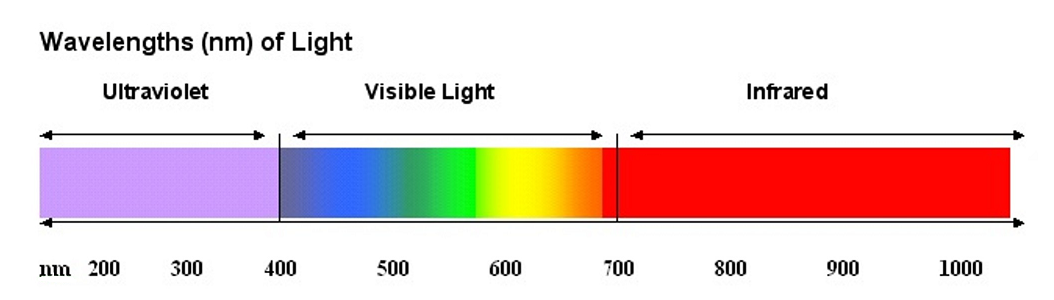
\includegraphics[scale=0.35]{images/ir_spectrum.png}
\caption{Wavelengths of light\\
Reproduced from \cite{ir_spectrum}}
\label{fig:ir_spectrum}
\end{figure}

\section{NDVI}

The normalized difference vegetation index (NDVI) is a simple graphical indicator that can be used to analyze remote sensing measurements, typically but not necessarily from a space platform, and assess whether the target being observed contains live green vegetation or not\cite{ndvi_wiki} as in Figure \ref{fig:ndvi_british}.

\begin{figure}[H]
\begin{subfigure}{0.5\textwidth}
\centering
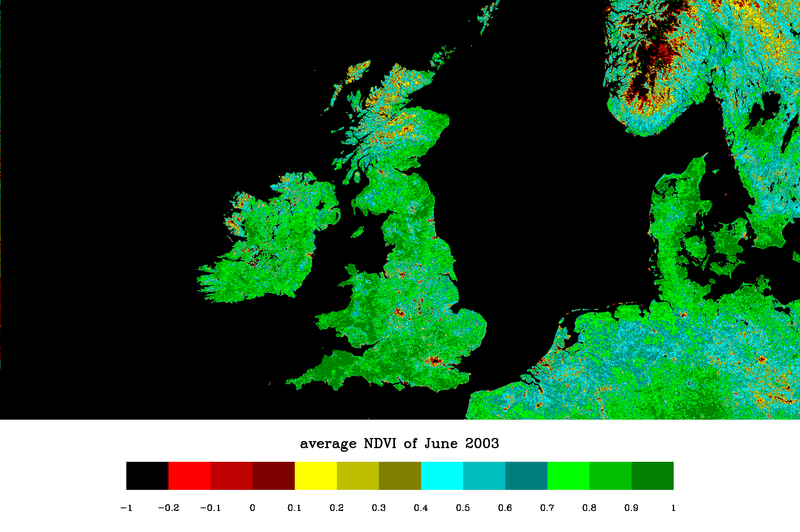
\includegraphics[scale=0.25]{images/NDVI_062003.png}
\caption{June 2003}
\end{subfigure}
\begin{subfigure}{0.5\textwidth}
\centering
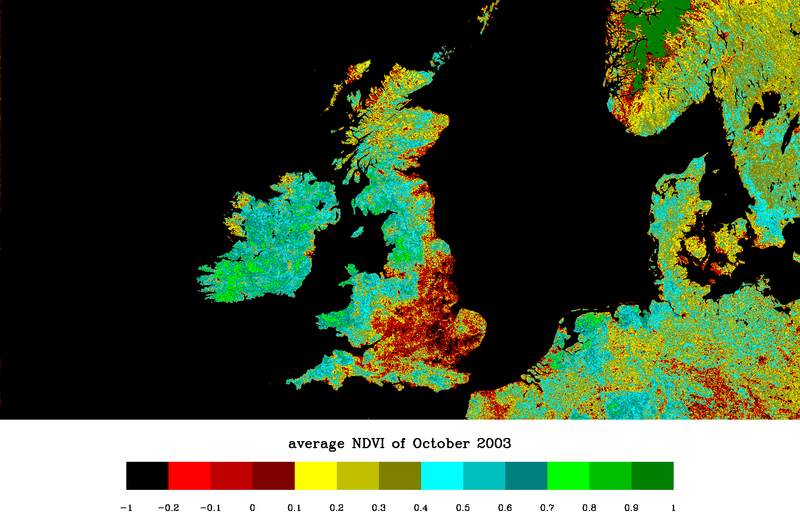
\includegraphics[scale=0.25]{images/NDVI_102003.png}
\caption{October 2003}
\end{subfigure}
\caption{Average NDVI over the British Isles\\
Reproduced from \cite{ndvi_wiki}}
\label{fig:ndvi_british}
\end{figure}

\noindent
The NDVI is calculated using the following formula for each pixel:\\

\begin{equation}\label{eq:ndvi}
{\displaystyle{\mbox{NDVI}}={\frac {({\mbox{NIR}}-{\mbox{Red}})}{({\mbox{NIR}}+{\mbox{Red}})}}}, \in [-1.0, 1.0]
\end{equation}

where red and NIR stand for the spectral reflectance measurements acquired in the red (visible) and near-infrared regions, respectively.

\begin{figure}[H]
\centering
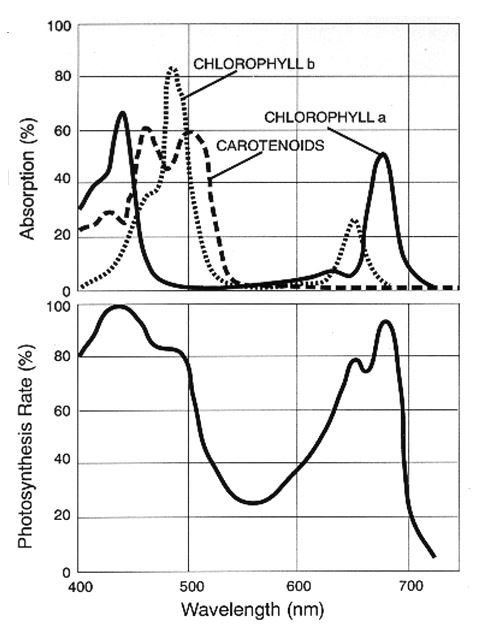
\includegraphics[scale=0.5]{images/chlorophyll.jpg}
\centering
\caption{PAR and absorption spectrum\\
Reproduced from \cite{ndvi_wiki}}
\label{fig:chlorophyll}
\end{figure}

In Figure \ref{fig:chlorophyll}, typical photosynthetic action in the photosynthetically active radiation (PAR) spectral region for live green plants is shown, beside absorption spectra for chlorophyll and carotenoids. Solar radiation is absorbed within this region as a source of energy. \\

Leaf cells re-emit solar radiation in the near-infrared region because the photon energy at wavelengths longer than 700 nm is not large enough to synthesize organic molecules, even though it comprises approximately half of the total incoming solar energy. If it were absorbed, it would only result in damage and overheating of the plant.\\

The NDVI is similar to a mere ratio of infrared light to visible light, yet since it is not normalised, one can have infinite values.\\

The rationale behind the NDVI is that one can exploit the strong differences in plant reflectance to determine their spatial distribution.\\

\section{Hardware Architecture}

\subsection{Filters}

A filter is needed to isolate the NIR channel. If a custom filter is used on a camera with the NIR filter removed, it is possible to isolate a NIR channel without visible light leakage on one or more colour channels. Variants include the Wratten 25A Red Long Pass filter, the Wratten 87 NIR All Pass filter and the Rosco 2008 Blue filter, which allow red and NIR light, only NIR light, and blue and NIR light respectively.\\

The Rosco 2008 Blue filter will be used, for most of the project, as well as the 600nm Dichroic Glass Longpass filter from Edmund Scientific, with limited access.

\subsection{Cameras}

Two cameras are required. It is seemingly impossible to capture pure NIR and pure red on separate channels unless the intrinsic bayer matrix is manufactured to allow for it, however, then it would not be cost effective (citation needed).\\

The Sony IMX219 series cameras will be used. They integrate with the Raspberry Pi using a single 15-pin CSI connection.

\subsection{Camera mount}

The cameras will be fixed relative to each other using a PCB substrate so that no rotational or translational drift can occur.

Also, the cameras are to be dampened to prevent a jello-effect due to the rolling shutter cameras. Global shutter cameras are more expensive.

\subsection{On-board processing}

This will be handled by two Raspberry Pis. Both will be used to take photos through each of their single CSI ports.

CSI port. Full access to camera and flight controller.

Initially, one raspberry pi was to be used with a camera multiplexer, but it didn't work, and therefore two raspberry pis were used. Just as well, as the flight controller uses all but 1 pin.

\subsection{Flight controller}

Flight controller is needed to stabilize the airborne vehicle, and set mission waypoints. The Raspberry Pi, Navio2, camera symbiosis was good since all three together are quite configurable, compared to other solutions.

\subsection{Drone}

A quadcopter was designed and built to handle all the equipment.

\subsection{Ground Control Station}

A 433 MHz linkup with a GCS is necessary for pre-flight checks, and monitoring/controlling the status of the vehicle during flight.

\section{Software Architecture}

\subsection{Flight controller}

A real-time kernel will be used for the Ardupilot Firmware used on the flight controller Raspberry Pi.


\subsection{Simultaneous camera triggering}

Linux. Initially TCP triggering was used, but the overhead and asynchronous nature meant that it was never consistently triggered at the same time. Instead, the clocks are sychronised using NTP, and attempt to trigger every second, on the second. The latter solution works quite well, with an occassional few milliseconds difference in stereo captures.

\subsection{Calibration}

Stereocalibration using chess board images was used.

\subsection{Stereorectification}

The images were undistorted according to the simultaneous chess board images it was calibrated at.

\subsection{SIFT and NDVI}

Finally, a scale-invariant-feature-transform is applied to the images to align them using an affine transform. An NDVI calculation is applied to the matched images, with a floating point output image. A LUT colourmap is applied to visibly distinguish different areas and their meanings in the final image.

\section{Stiching and Mapping}

A few images are stitched together to show proof-of-concept.
\label{chapter:sysarch}
\chapter{Drone Design and Construction}

A drone is designed and constructed. The goal is to be cost-effective and to source local supplies. It should be noted that pre-built drones like the DJI Phantom and Inspire cost significantly more\footnote{Easily 100\% to 200\% more}. See Appendix \ref{app:bom} for a Bill of Materials.

\section{Drone}

\subsection{Mechanical subsystem design}

The drone will be medium sized, with a payload of 500-1000g. It would be ideal to have a good thrust to weight ratio of 3:1.

\subsubsection{Frame}

There are many materials and configurations for a drone. The configurations include 3, 4, 6, 8 arms or more, with single or contra-rotating propellers on each arm\footnote{Two propellers aligned vertically and spinning opposite to each other for upwards thrust}. \\

In aerial cinematography, it would require a stiff but less brittle frame as in Figure \ref{fig:hex} to provide a smooth and stable flight. They also need to be large enough to hold the cameras needed for this professional activity. Lastly, the frames should be supportive of tall landing gear \cite{frame}. Due to the larger overall mass, the frame's natural frequency is low, meaning that it provides the same stability as a hand-held weighted gimbal in cinematography. For our application, we'll be using lightweight cameras, which weigh 3 grams each, which means our drone can be lighter.\\

\begin{figure}[H]
\begin{subfigure}{0.5\textwidth}
\centering
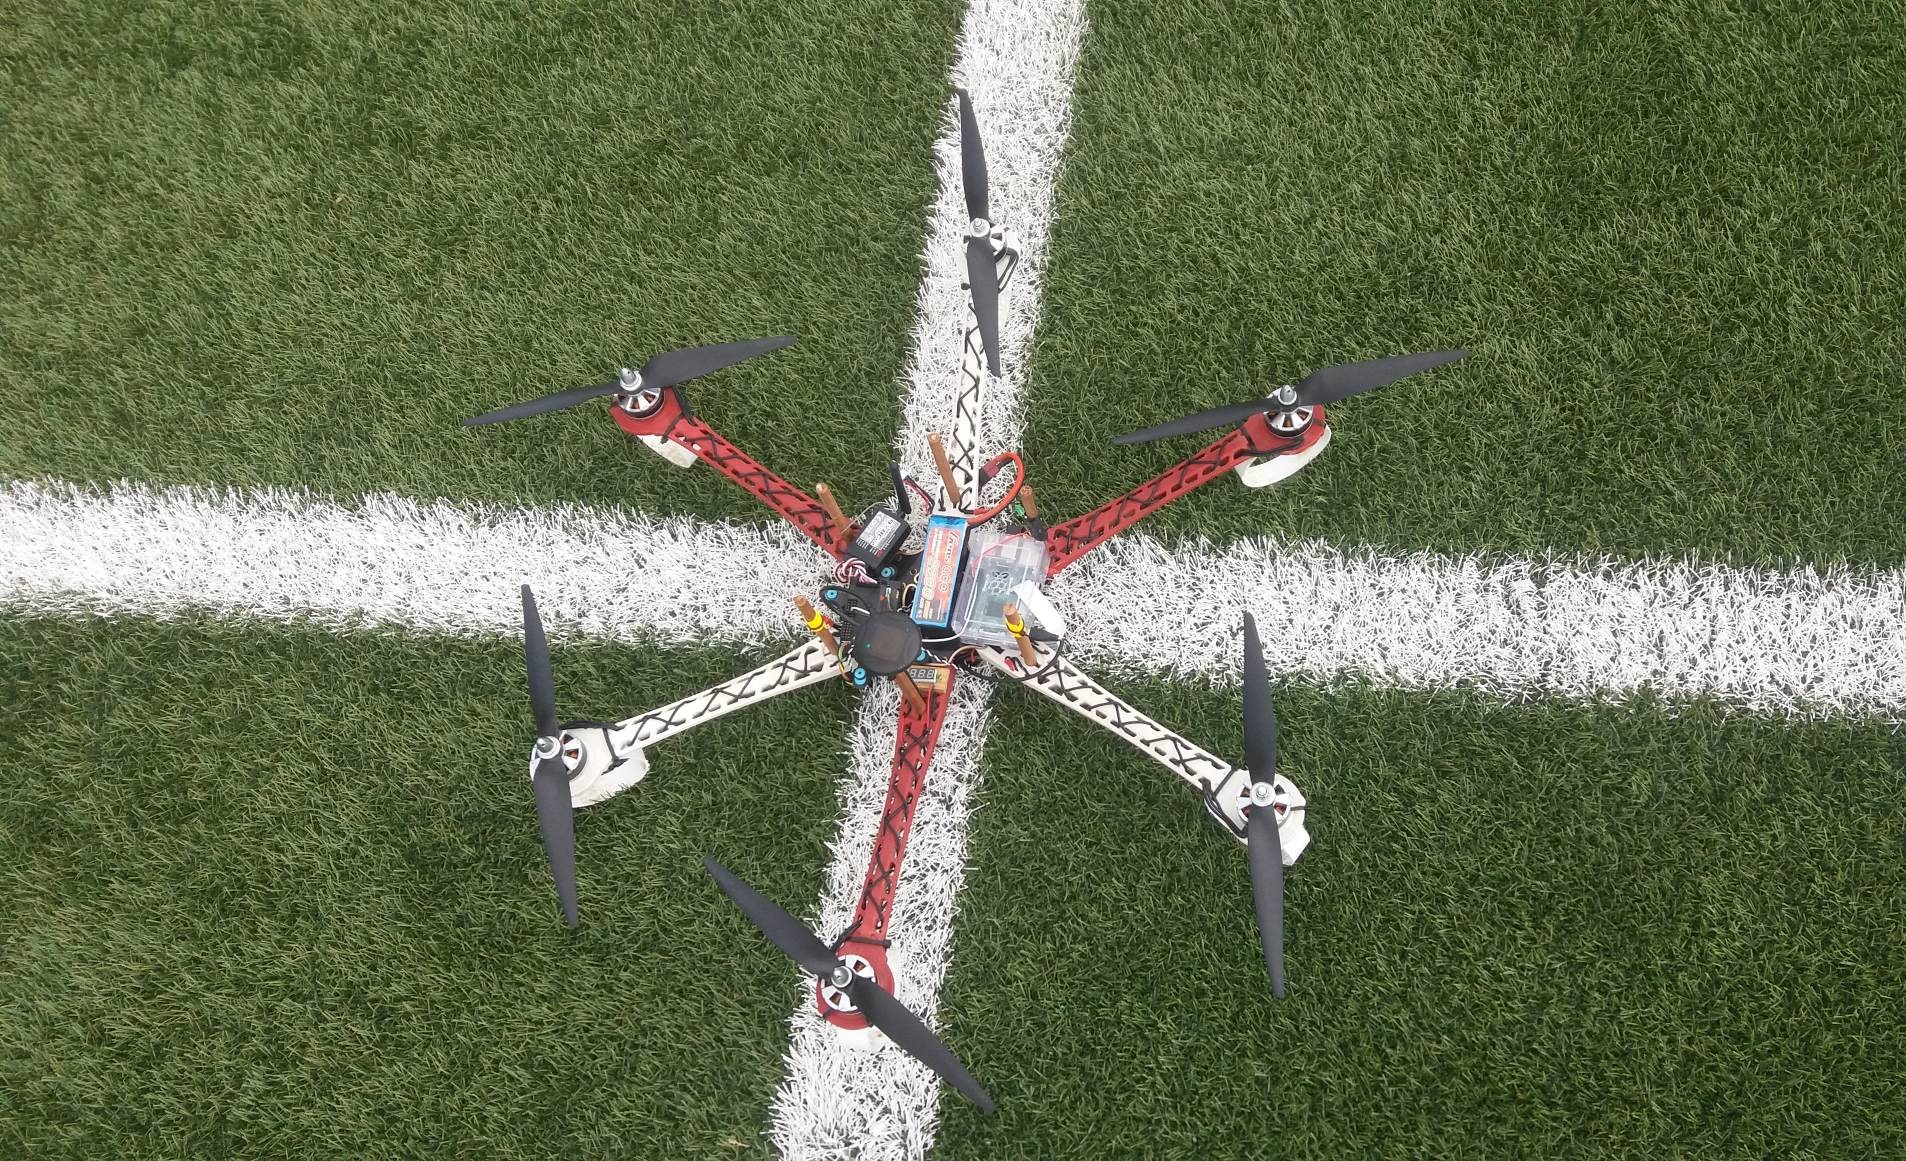
\includegraphics[scale=0.11]{images/hex3.jpg}
\caption{Hex multirotor landed}
\end{subfigure}
\begin{subfigure}{0.5\textwidth}
\centering
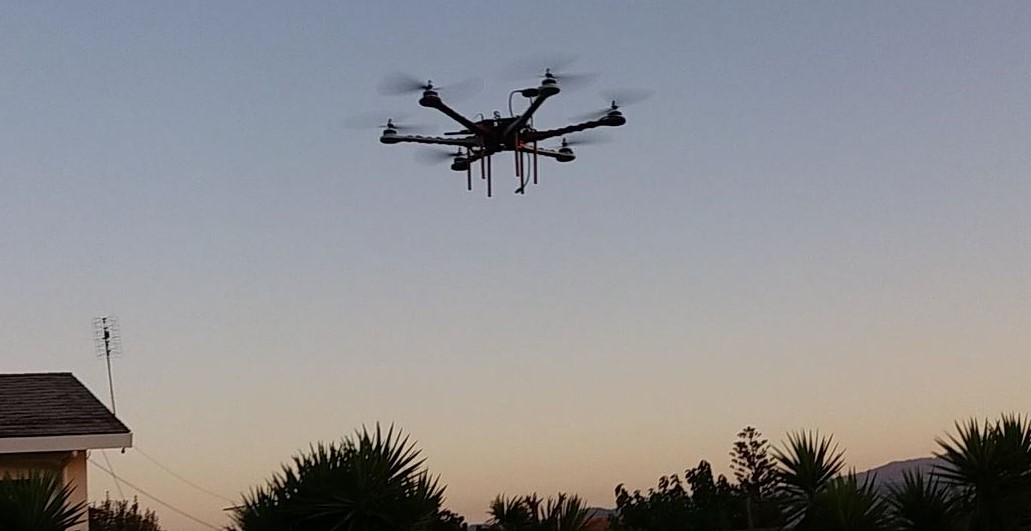
\includegraphics[scale=0.3]{images/hex2.jpg}
\caption{Hex multirotor in-flight}
\end{subfigure}
\caption{Large cinematography multirotor}
\label{fig:hex}
\end{figure}

Recreational usage may use 'mini multicopter frames' for flying indoors and outdoors \cite{frame} as in Figure \ref{fig:small_quad}. They're extremely light, but do not have enough space or power for other peripherals\footnote{GPS, Raspberry Pis etcetra}.\\

\begin{figure}[H]
\centering
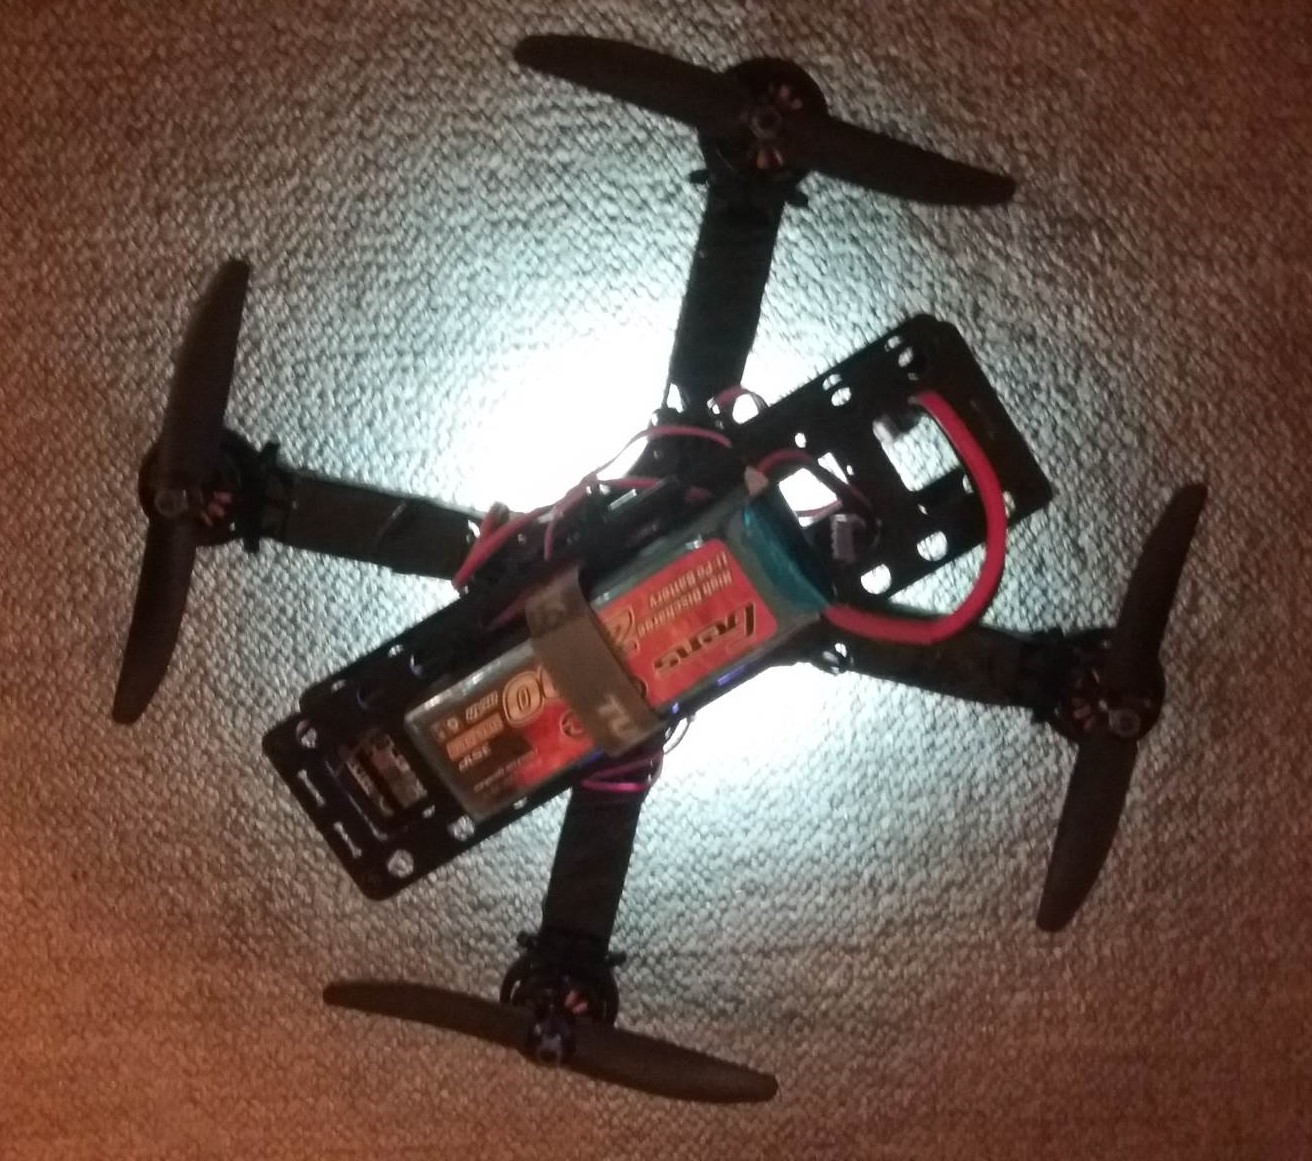
\includegraphics[scale=0.12]{images/small_quad.jpg}
\caption{Small recreational quadcopter}
\label{fig:small_quad}
\end{figure}

Sports drones are light and fast, but they require high discharge batteries. Like the quadcopter\footnote{Four propellers. Hex is 6, and `multirotors' have any number more than 2.} in Figure \ref{fig:small_quad} which has 2300 KV\footnote{KV is not kilo-volts. It is a measure of the revolutions per minute when 1 Volt is applied with no load attached to the motor} rated motors, sports/racing drones also have 2000+ KV ratings, but they will typically have thicker windings, which means it is capable of a higher wattage. One may be able to make enough room, but the batteries will not last very long.\\

A combination of these configurations means that a medium sized quadcopter/drone will be suitable. It is not too light or too heavy, and has room and power for other peripherals.\\

Materials include carbon-fibre, aluminium, fibreglass and synthetic polymers. The differences between them are not major, except that aluminium is heavier, requires larger motors and induces more vibrations. Carbon-fibre contributes to radio interference\cite{frame}, but is the lightest.\\

The closest local-supplier competition before the F450-V2 quadcopter frame was chosen was the ZMR250 Carbon Mini Quad FPV Frame as in Figure \ref{fig:zmr}.

\begin{figure}[H]
\centering
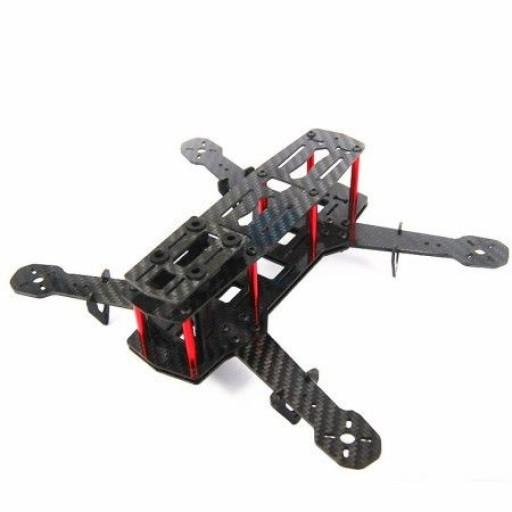
\includegraphics[scale=0.35]{images/zmr250.jpeg}
\caption{ZMR250 Carbon Mini Quad FPV Frame \cite{frobot}}
\label{fig:zmr}
\end{figure}

Both frames have roughly the same price\footnote{500 ZAR}. The ZMR250 has a carbon fibre body making it extremely light (145g), but fell into the class of `mini multicopter' as mentioned earlier. Therefore due to its local availability and accommodating space, the F450-V2 frame was chosen as in Figure \ref{fig:frame}.

\subsubsection{Landing Gear}

Four lengths of 10mm pine dowels approximately 15mm long were used. They totalled about 10 ZAR. The frame has 5cm legs, but accomodation has to be made for the nadir cameras.

\subsubsection{Motors}

The motors are rated at 920 KV and 230 W. This is relatively low compared to the more common racing motors with around 2000 KV or more (which the ZMR250 frame would use). KV is related to the power output and torque level of a motor. This is determined by the number of turns on the armature and the strength of the magnets.\\

\begin{figure}[H]
\centering
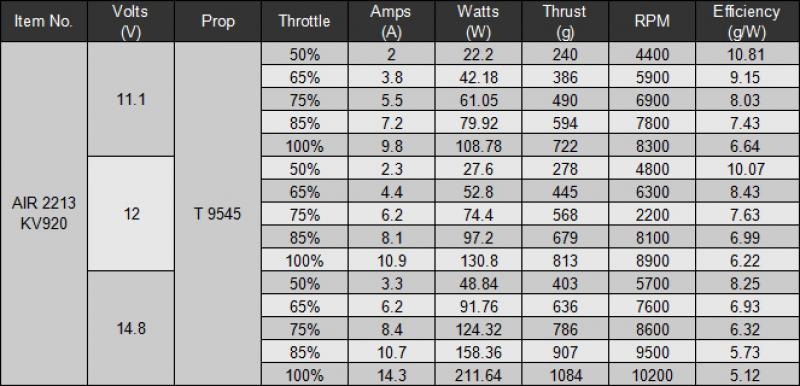
\includegraphics[scale=0.4]{images/motor_specs.jpg}
\caption{Motor and propeller combination specifications \cite{frobot}}
\label{fig:mot_prop_specs}
\end{figure}

Besides the many other characteristics, at maximum throttle, and using 3 cell batteries, the thrust is determined to be 3252 g in Figure \ref{fig:mot_prop_specs}. This gives a thrust to weight ratio of 2.95, which is satisfactory.

\subsubsection{Propellers}

The propellers have a pitch of 4.5', which is basically a measure of the 'bite', or distance it travels through the air on one revolution.

\subsubsection{Protective enclosure}

A housing is needed to protect the exposed electronics from the elements. Also, dramatic airflow can affect the barometer readings. A case \cite{3d_case} was 3D printed for the Navio2 and Raspberry Pi as in Figure \ref{fig:fcarpc2}.

\begin{figure}[H]
\begin{subfigure}{0.5\textwidth}
\centering
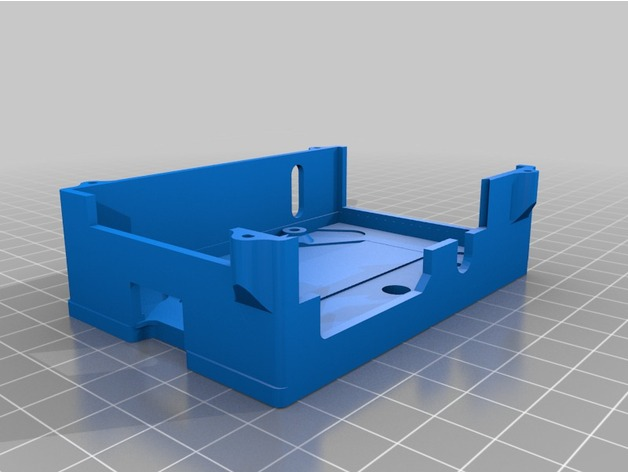
\includegraphics[scale=0.25]{images/drone-build-3d-case-render.jpg}
\caption{Case render}
\label{fig:fcarpc1}
\end{subfigure}
\begin{subfigure}{0.5\textwidth}
\centering
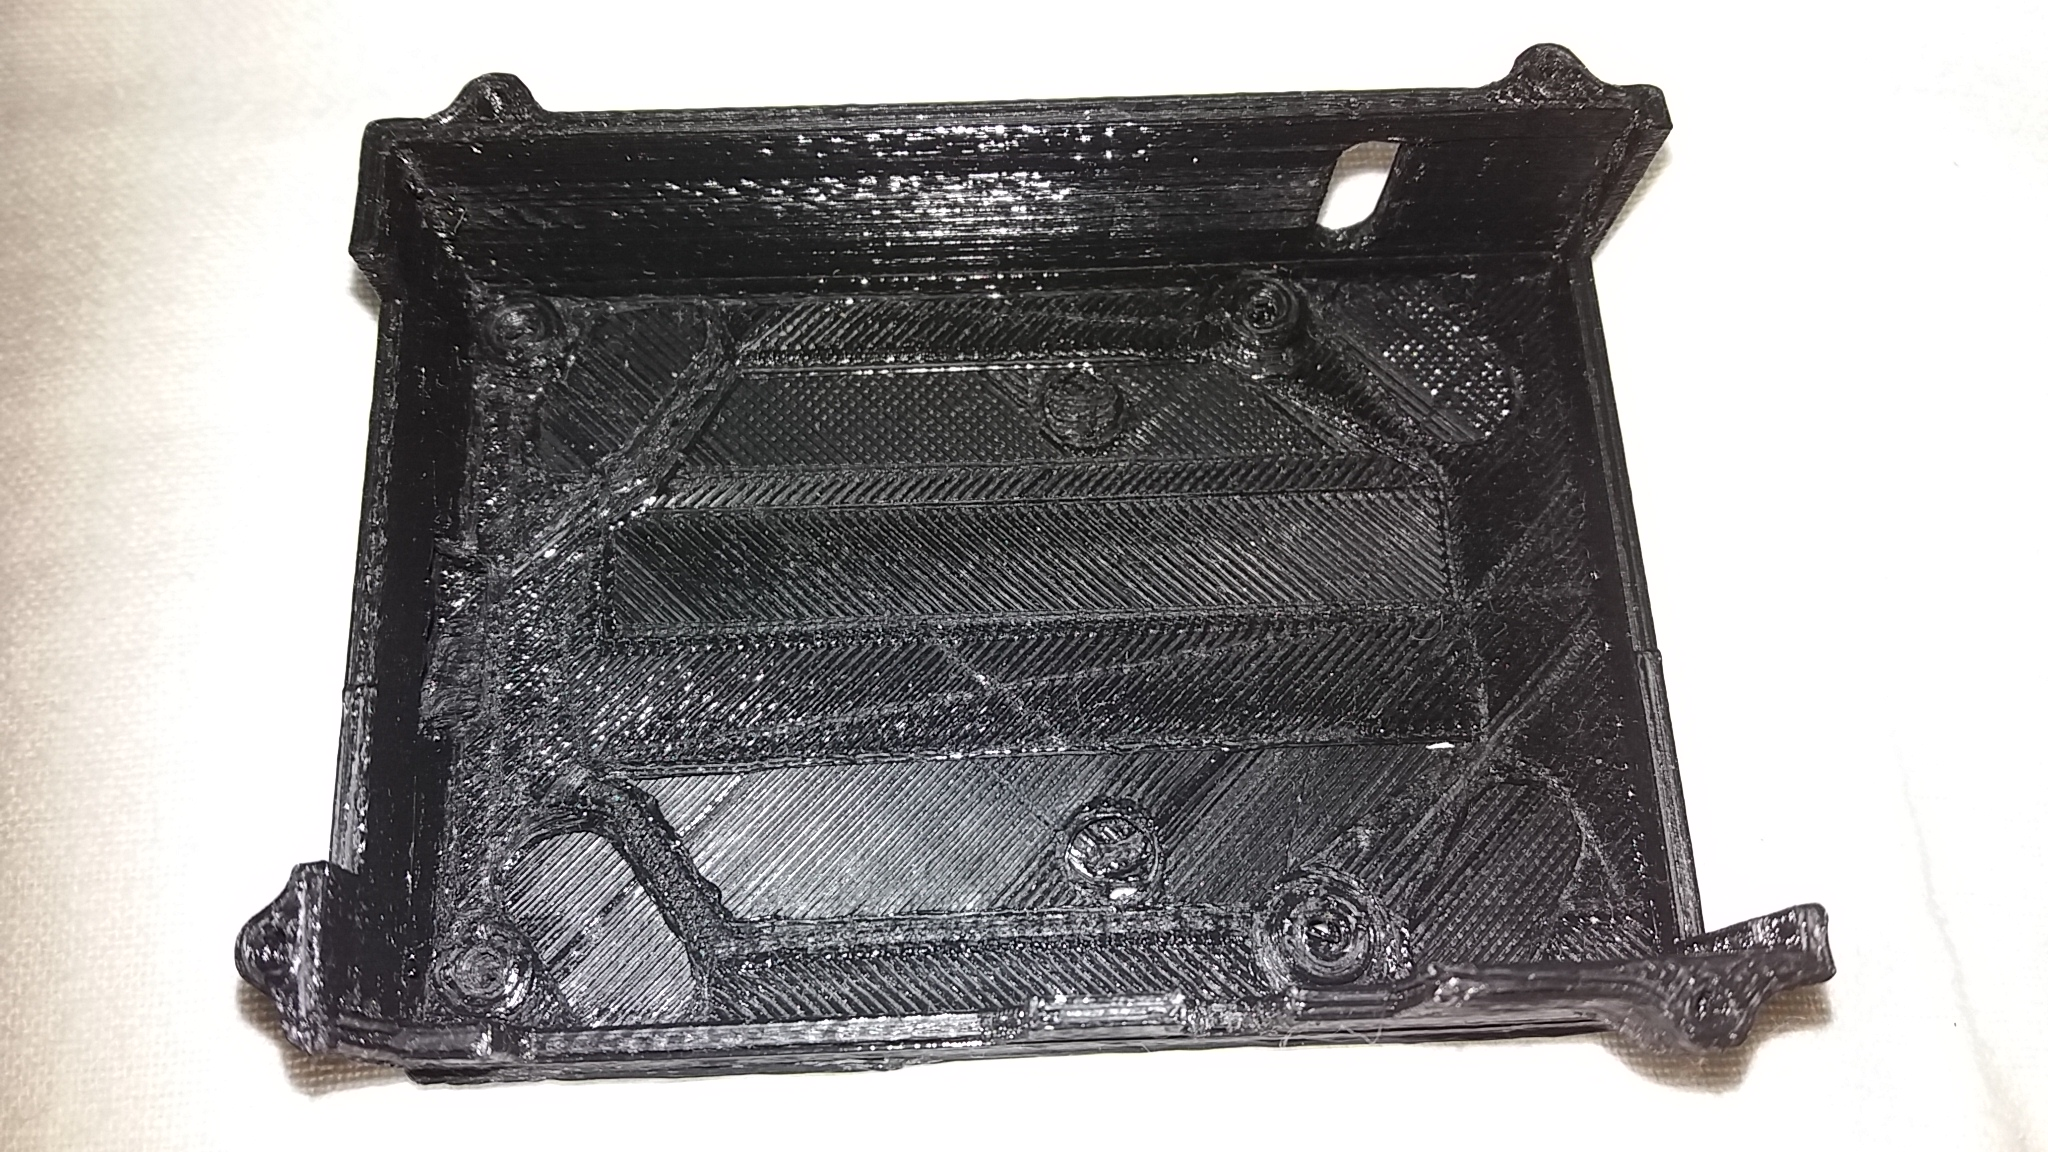
\includegraphics[scale=0.1]{images/drone-build-3dcase.jpg}
\caption{3D printed case for Raspberry Pi and Navio2.}
\label{fig:fcarpc2}
\end{subfigure}
\caption{Flight controller and Raspberry Pi case}
\label{fig:fcarpc}
\end{figure}

\subsection{Electrical subsystem design}
\subsubsection{Batteries}

Multiple 3S1P batteries will be used as in Figure \ref{fig:batteries}, since the price cost-point was the cheapest from Goblin Hobbies.\\

\begin{figure}[H]
\centering
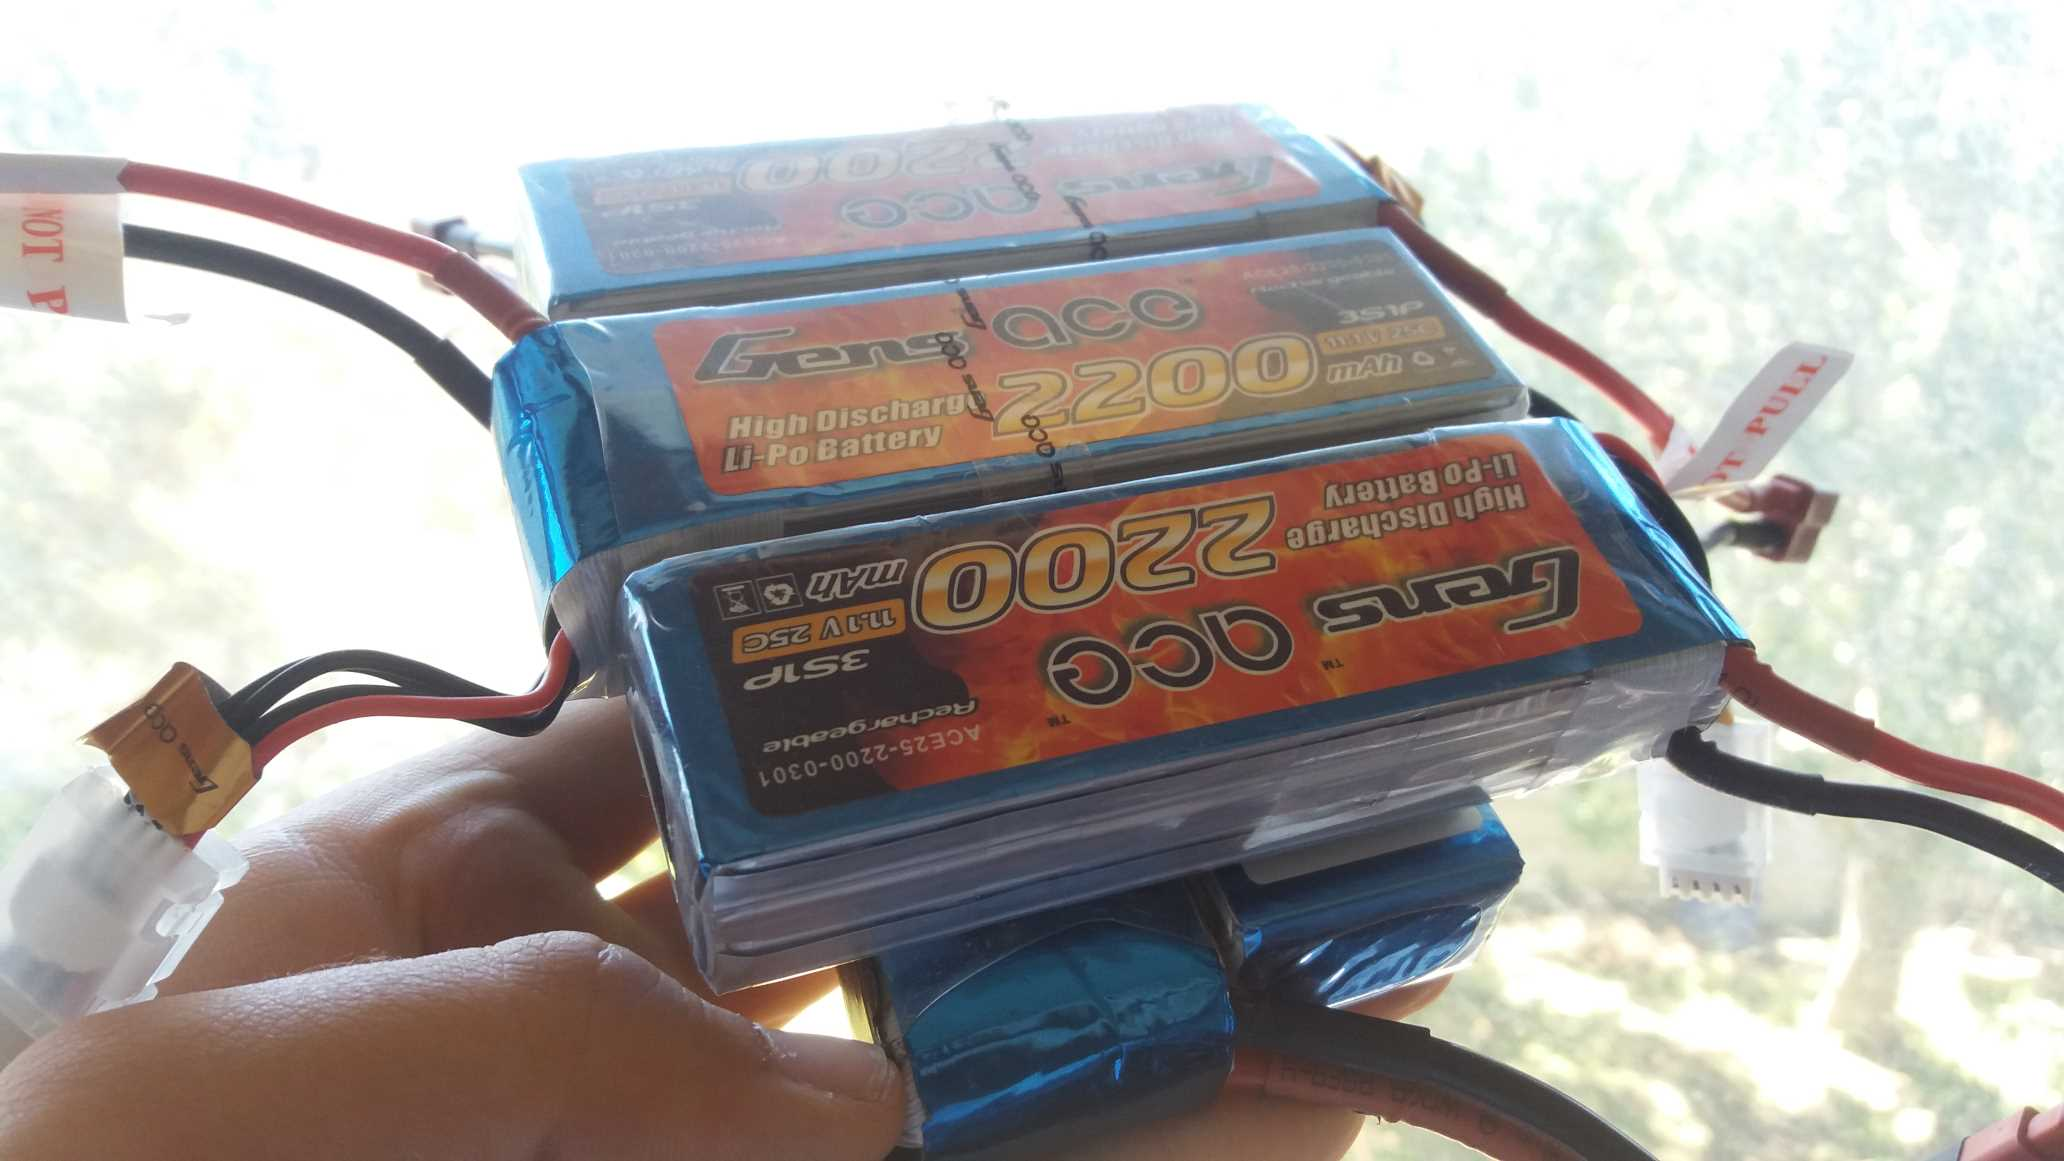
\includegraphics[scale=0.17]{images/batteries.jpg}
\caption{3SP1 GensAce Lithium batteries}
\label{fig:batteries}
\end{figure}

They are charged using a balance-charger, which charges all three cells equally so that they all age the same. Otherwise cells may burst, or cause damage due to the discrepancies.\\

With an average current draw of 20 A, each battery will only last 6.6 minutes, but long missions can be interrupted easily as noted in Section \ref{sec:dual_power}.

\subsubsection{Dual power redundancy}
\label{sec:dual_power}

The flight controller takes in two power source inputs for dual redundancy as in Figure \ref{fig:dual_redundancy}. One of the batteries powers the motors during flight. This also allows the electronics to remain on when swapping out the flight battery.

\begin{figure}[H]
\centering
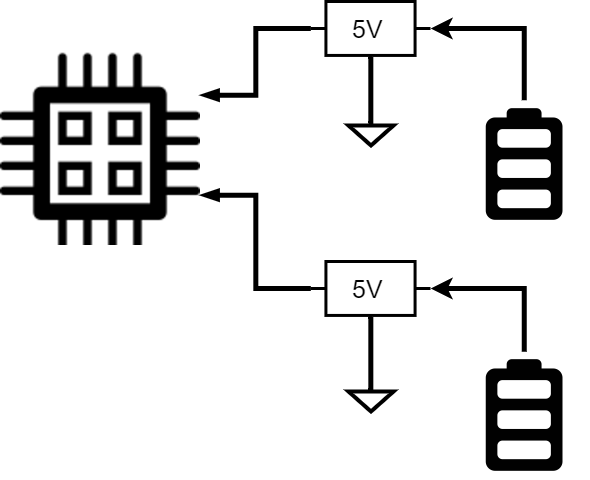
\includegraphics[scale=0.35]{images/dual_redundancy.png}
\caption{Illustrating dual power redundancy}
\label{fig:dual_redundancy}
\end{figure}

\subsubsection{Electronic speed controllers}

The 3-phase motors require speed control. This is achieved by ESCs. Maximum power draw from the motors is 18A. 20A rated ESCs are used.

\subsection{Processor subsystem design}

The Navio2 flight controller fits perfectly onto the Raspberry Pi's 40-pin header in Figure \ref{fig:insertion_navio}. It also uses every signal pin, except for one. The Navio2 communicates directly with the Broadcom CPU on the Pi, resulting in a multi-processor system. The greatest significance in this case is that flight variables can be monitored and controlled. It is non-trivial in standalone flight controllers, as the on-board firmware has to be modified with utmost care.\\

The Navio2 has a co-processor to handle PPM/Sbus inputs and provides PWM output for the ESCs.

\subsection{Control subsystem design}

\subsubsection{Flight controller}
Flight controller is needed to stabilize the airborne vehicle, and set mission waypoints. The Raspberry Pi, Navio2, and camera symbiosis was good since all three together are quite configurable even during flight, compared to other solutions which require hands-on intervention.\\

The Navio2 was chosen specifically for its harmonious relationship with the Raspberry Pi.

\subsubsection{Flight modes}

Loiter mode uses GPS to maintain altitude and location. Altitude hold only uses the barometer. Stabilize mode gives the pilot full control of the throttle, and can be used to quickly change height, albeit it is a bit dangerous. Auto mode is used to fly autonomously in missions. Return to launch (RTL) uses GPS and does as its namesake suggests. Brake mode is used to pause its current activity, and if moving quickly it will actively brake by tilting in the other direction to prevent drift. All these flight modes can be accessed in flight by the remote controller, except Auto mode which is activated using the GCS.

\subsection{Communication subsystem design}
\label{sec:comms}

The drone communicates with the handheld remote controller via S-BUS, which is a universal standard. The beauty of it is that it communicates with one signal wire as in Figure \ref{fig:attach_sbus}. Previous implementations one may have had to use pulse position modulation (PPM), where each channel requires a wire. Even though this may sound simple, it does increase PCB size, complexity and cost in the end. One the same note, each electronic speed controller (ESC) gets a signal wire and power input.

%(add picture showing all the wireless technologies)\\

The drone can communicate via wifi as its medium of wireless telemetry; but the interference from other devices in the crowded 2.4 GHz ISM band drastically reduces range -- especially from the handheld remote controller. That, and the wifi dongles that were available seemed to work only for about 10 m.\\

Thus, 433 MHz 100mW transceivers were connected between the GCS and the drone as in Figure \ref{fig:attach_433}, at a 56400 baudrate. Real-time telemtery to a ground station is useful for pre-flight checks, in-flight monitoring and control, and missions.\\

For development purposes, wifi is used extensively to SSH into the Raspberry Pis and to analyse photos using SAMBA. It should be noted that due to the conflict with the remote controller, it is not possible to view photos in-flight. Nevertheless, there are many cases where the wifi disconnects, and it was required to have a script running to reconnect the wifi whenever it goes down (see code in appendix \ref{code:wifiup}).\\

The flight controller controls the ESCs via PWM signals as in Figure \ref{fig:pwm}. Likewise, the remote controller (as in Section \ref{sec:remote_controller}) also sends the PWM values of each channel, yet via SBus (a single-wire form of uart communication). SBus supports up to 18-channels.\\

\begin{figure}[H]
\centering
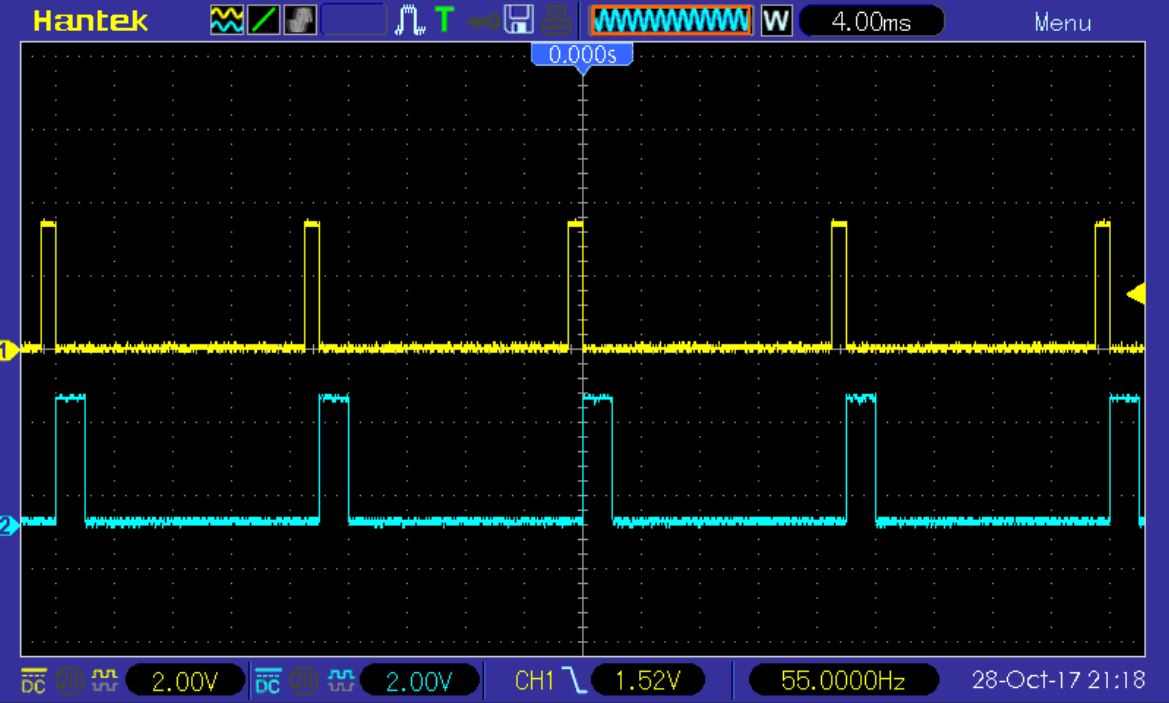
\includegraphics[scale=0.35]{images/pwm.jpg}
\caption{Min (yellow) and max (blue) duty cycle of PWM}
\label{fig:pwm}
\end{figure}

The PWM has a wavelength of 18 ms, and a duty cycle between 1 ms and 2 ms.

\subsection{Sensor subsystem design}

The flight controller has dual IMUs for redundancy, a GNSS receiver and a high resolution barometer for 10cm altitude resolution.

\begin{enumerate}
\item MPU9250 9DOF IMU
\item LSM9DS1 9DOF IMU
\item MS5611 Barometer
\item U-blox M8N Glonass/GPS/Beidou
\end{enumerate}

\subsection{Construction process and Integration}

At first, the frame is put together. This gives one a good idea of the actual size from the beginning.

\begin{figure}[H]
\begin{subfigure}{0.5\textwidth}
\centering
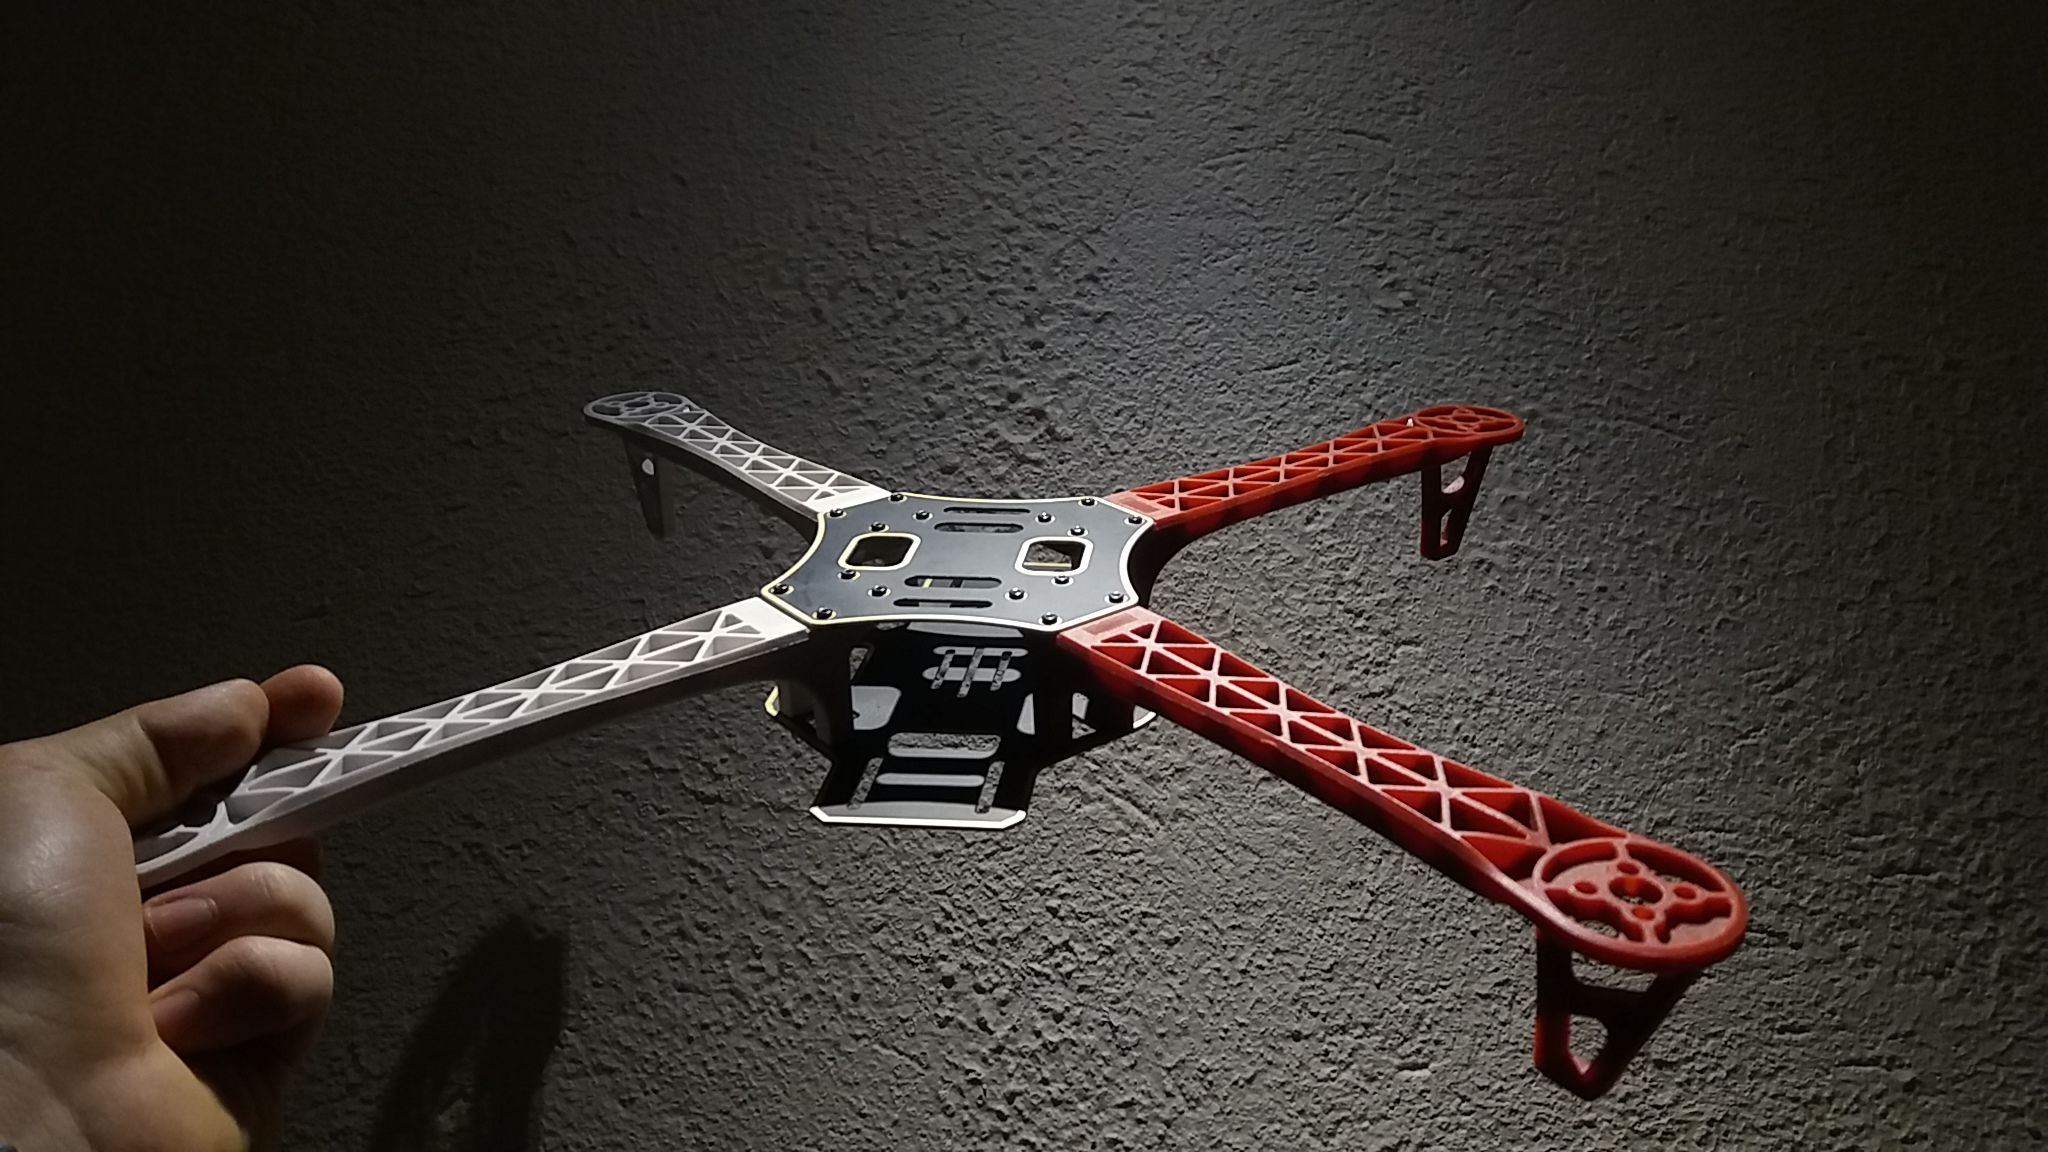
\includegraphics[scale=0.1]{images/drone-build-frame.jpg}
\caption{F450-V2 frame.}
\label{fig:frame}
\end{subfigure}
\begin{subfigure}{0.5\textwidth}
\centering
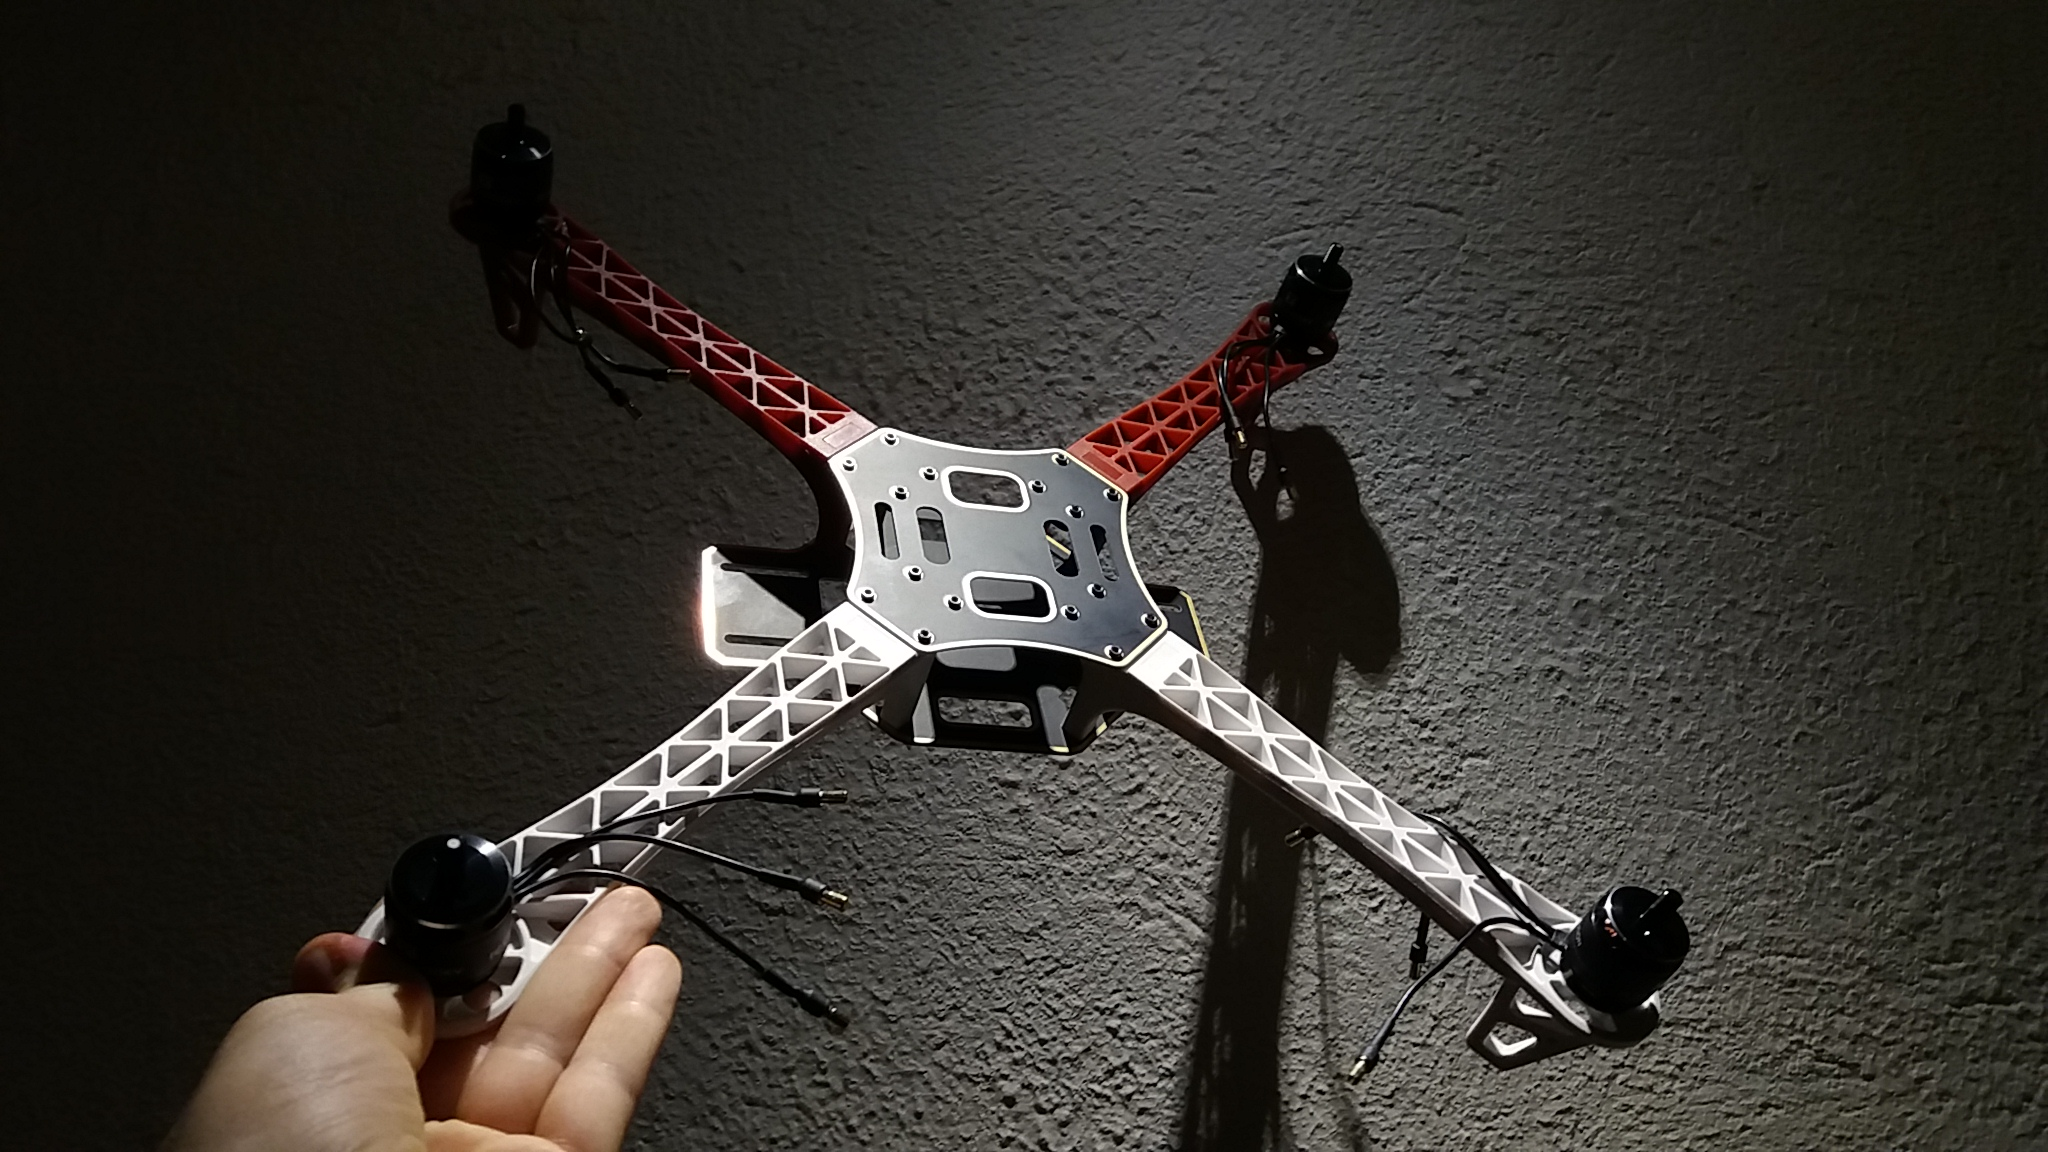
\includegraphics[scale=0.1]{images/drone-build-motors.jpg}
\caption{Adding the 920kv motors.}
\label{fig:motors}
\end{subfigure}
\caption{Frame and motors}
\label{fig:frame_motors}
\end{figure}

The nylon polymer frame as in Figure \ref{fig:frame} seems surprisingly robust, especially considering that the centre is PCB based.\\

\begin{figure}[H]
\begin{subfigure}{0.5\textwidth}
\centering
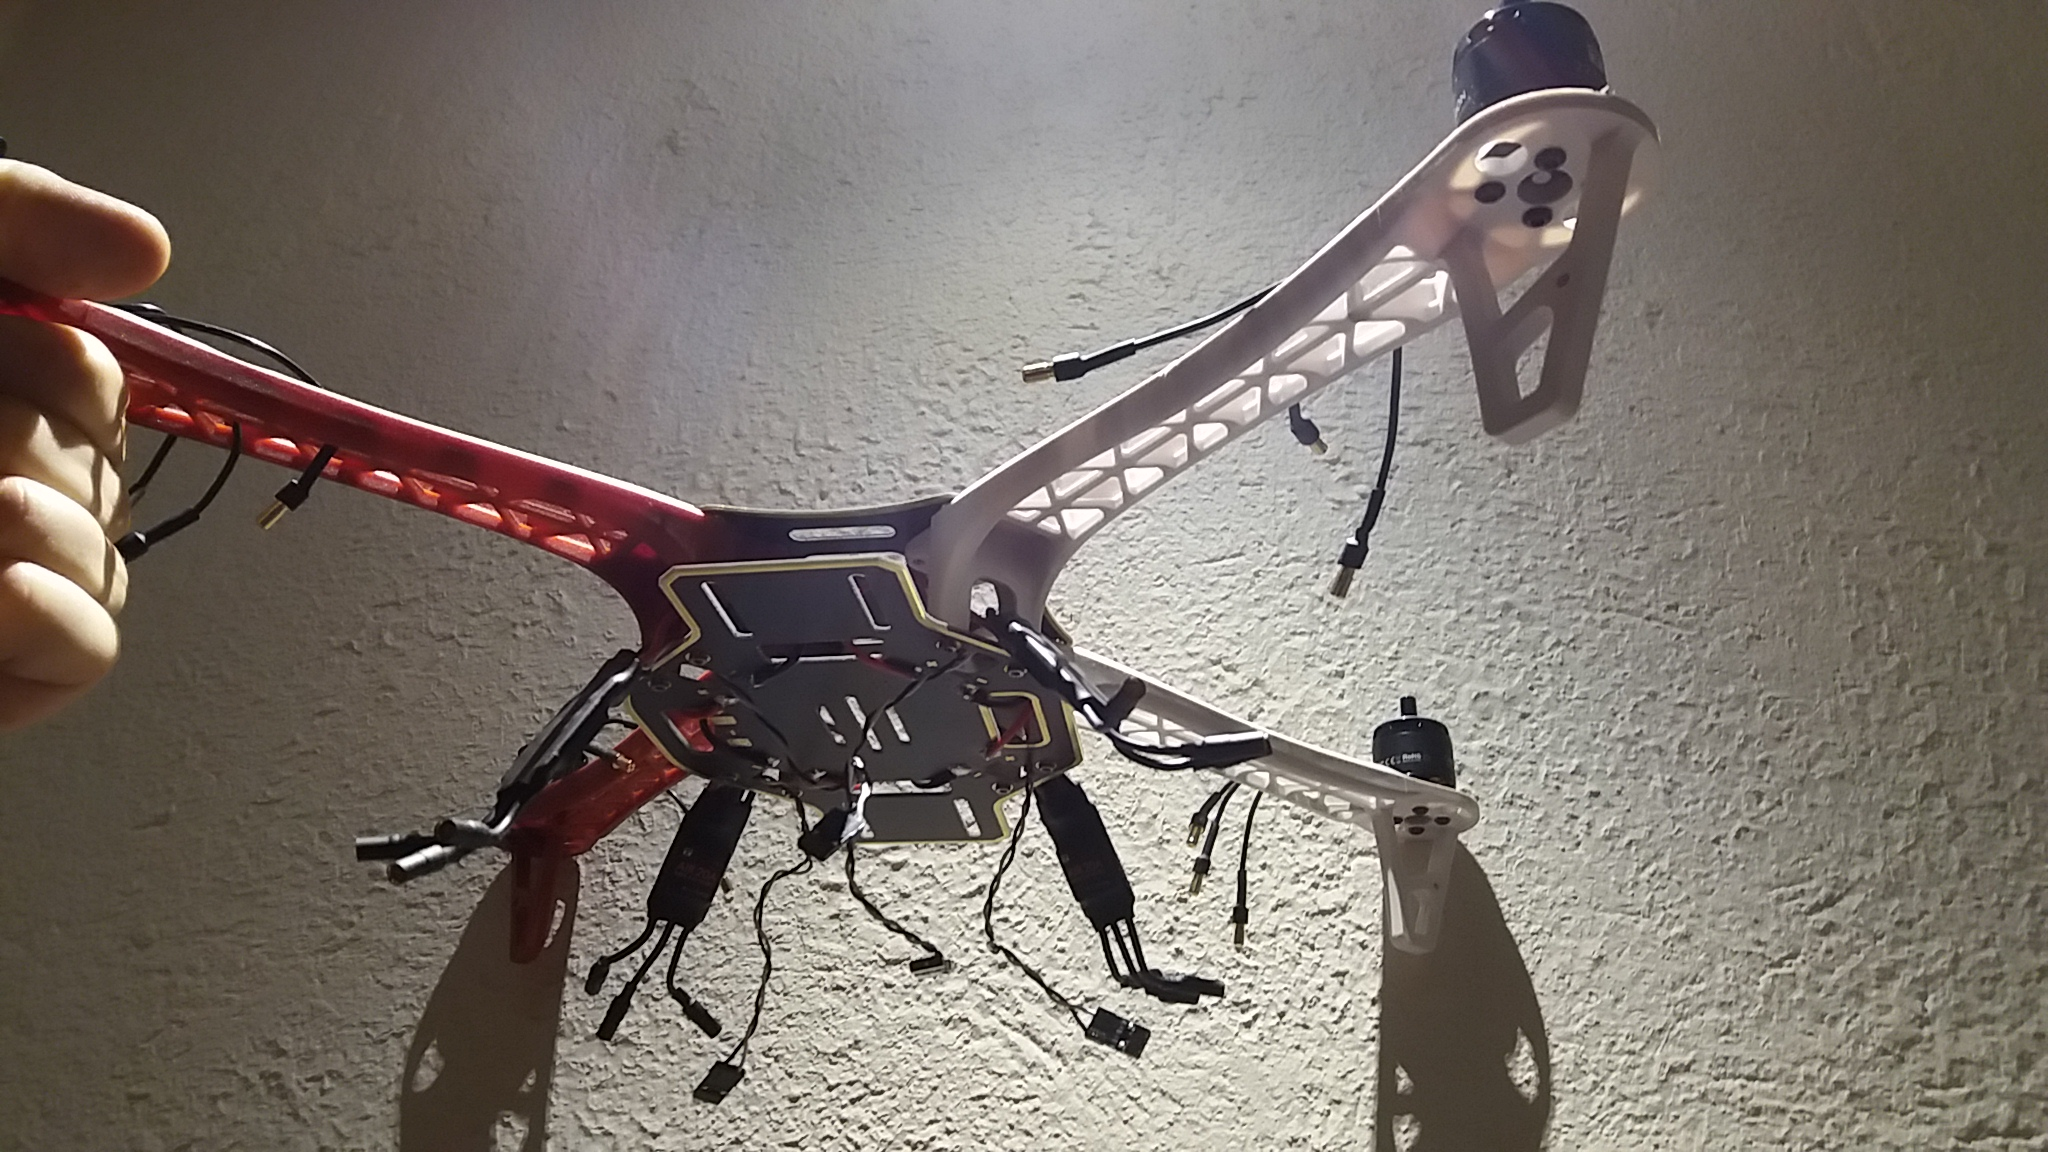
\includegraphics[scale=0.1]{images/drone-build-esc-3phaseunconnected.jpg}
\caption{Adding the ESCs. Motors require 3-phase power}
\label{fig:ESCs_uplugged}
\end{subfigure}
\begin{subfigure}{0.5\textwidth}
\centering
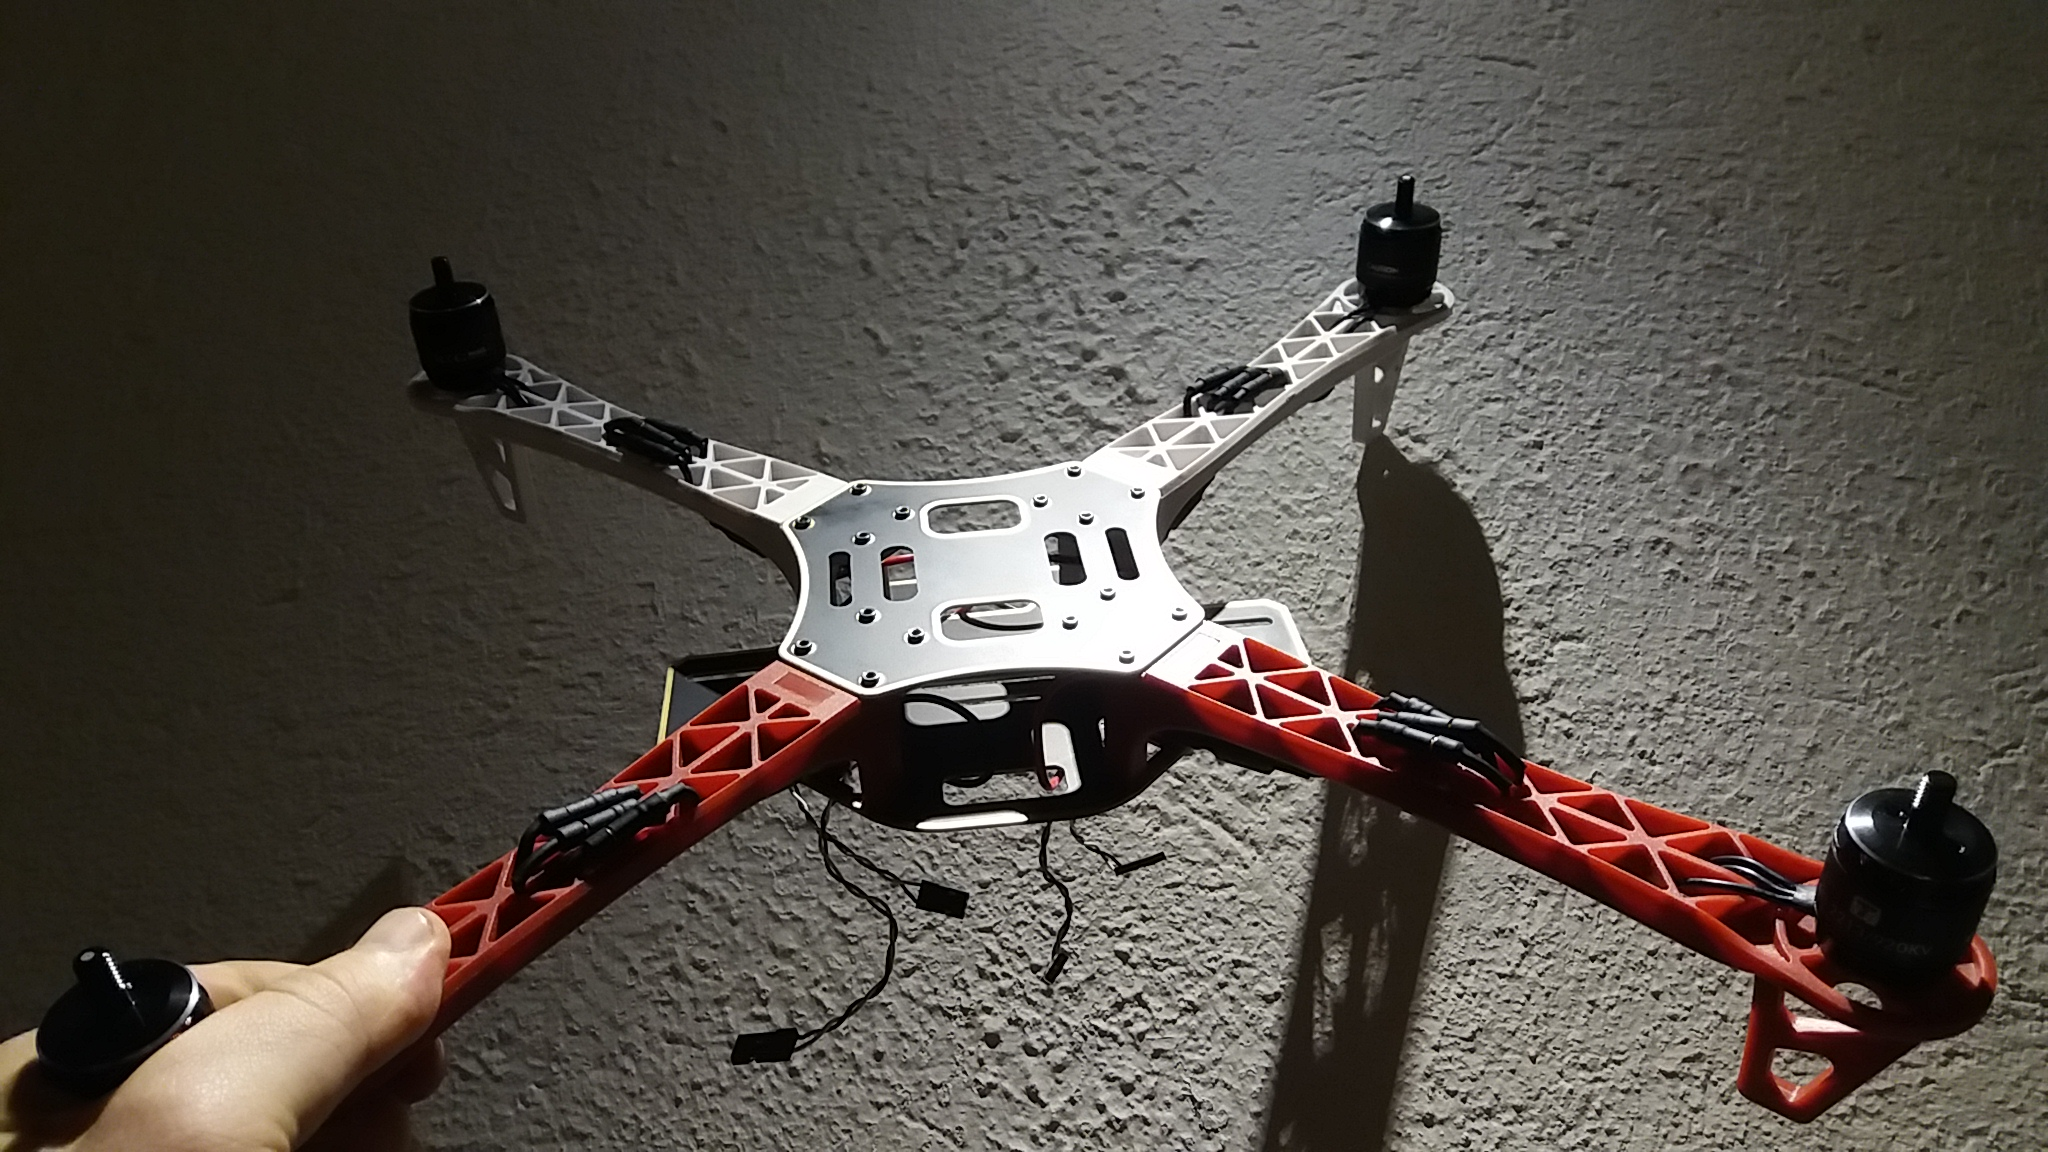
\includegraphics[scale=0.1]{images/drone-build-esc-3phaseconnected.jpg}
\caption{Power leads plugged in and secured}
\label{fig:ESCs_plugged}
\end{subfigure}
\caption{ESCs}
\label{fig:ESC}
\end{figure}

The leads are easy to plug/unplug. Any two phase leads can be swapped to change motor direction as in Figure \ref{fig:ESC}.\\

\begin{figure}[H]
\begin{subfigure}{0.5\textwidth}
\centering
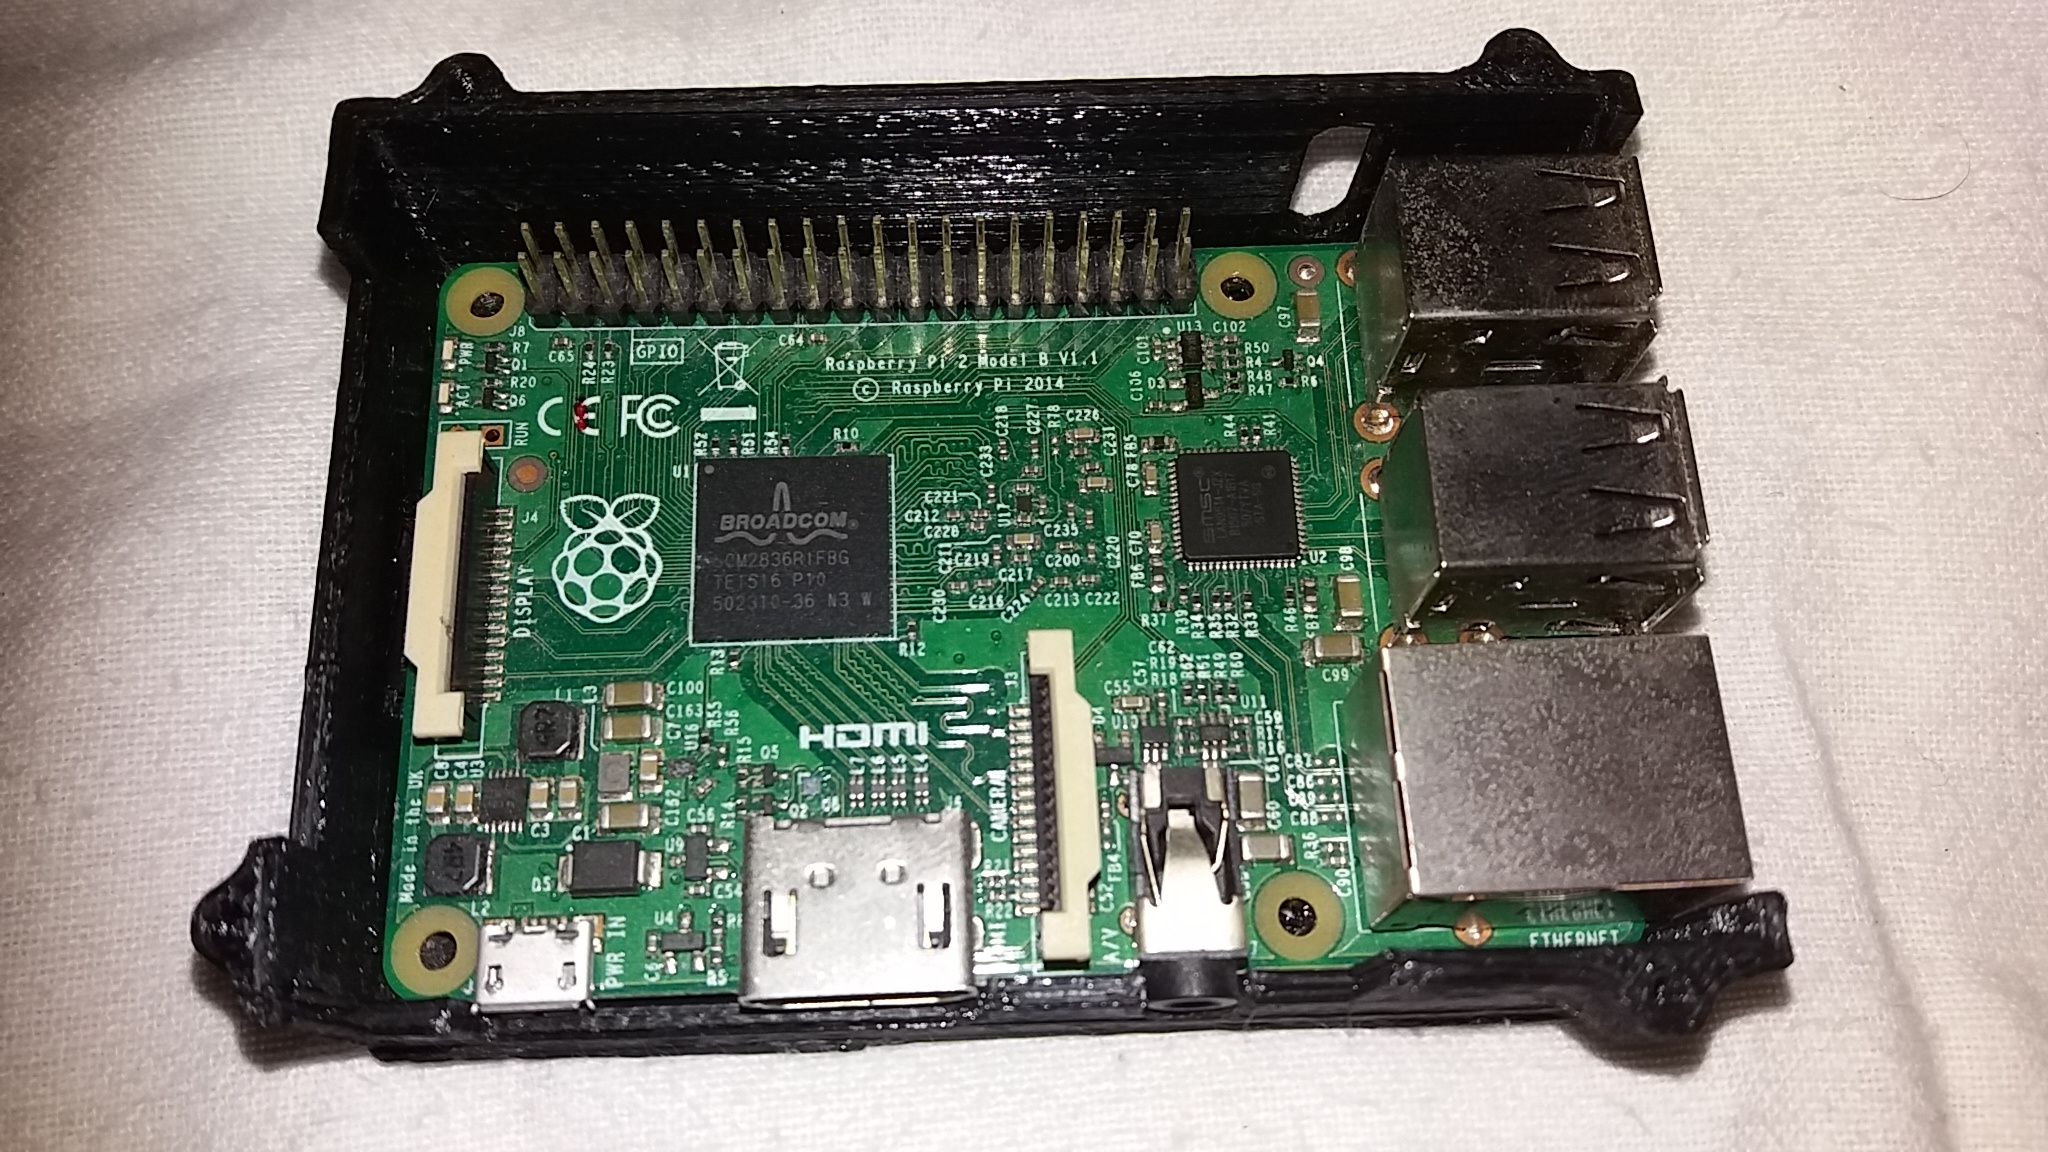
\includegraphics[scale=0.1]{images/drone-build-3dcase-pi.jpg}
\caption{Putting the Pi in the case.}
\label{fig:insertion_pi}
\end{subfigure}
\begin{subfigure}{0.5\textwidth}
\centering
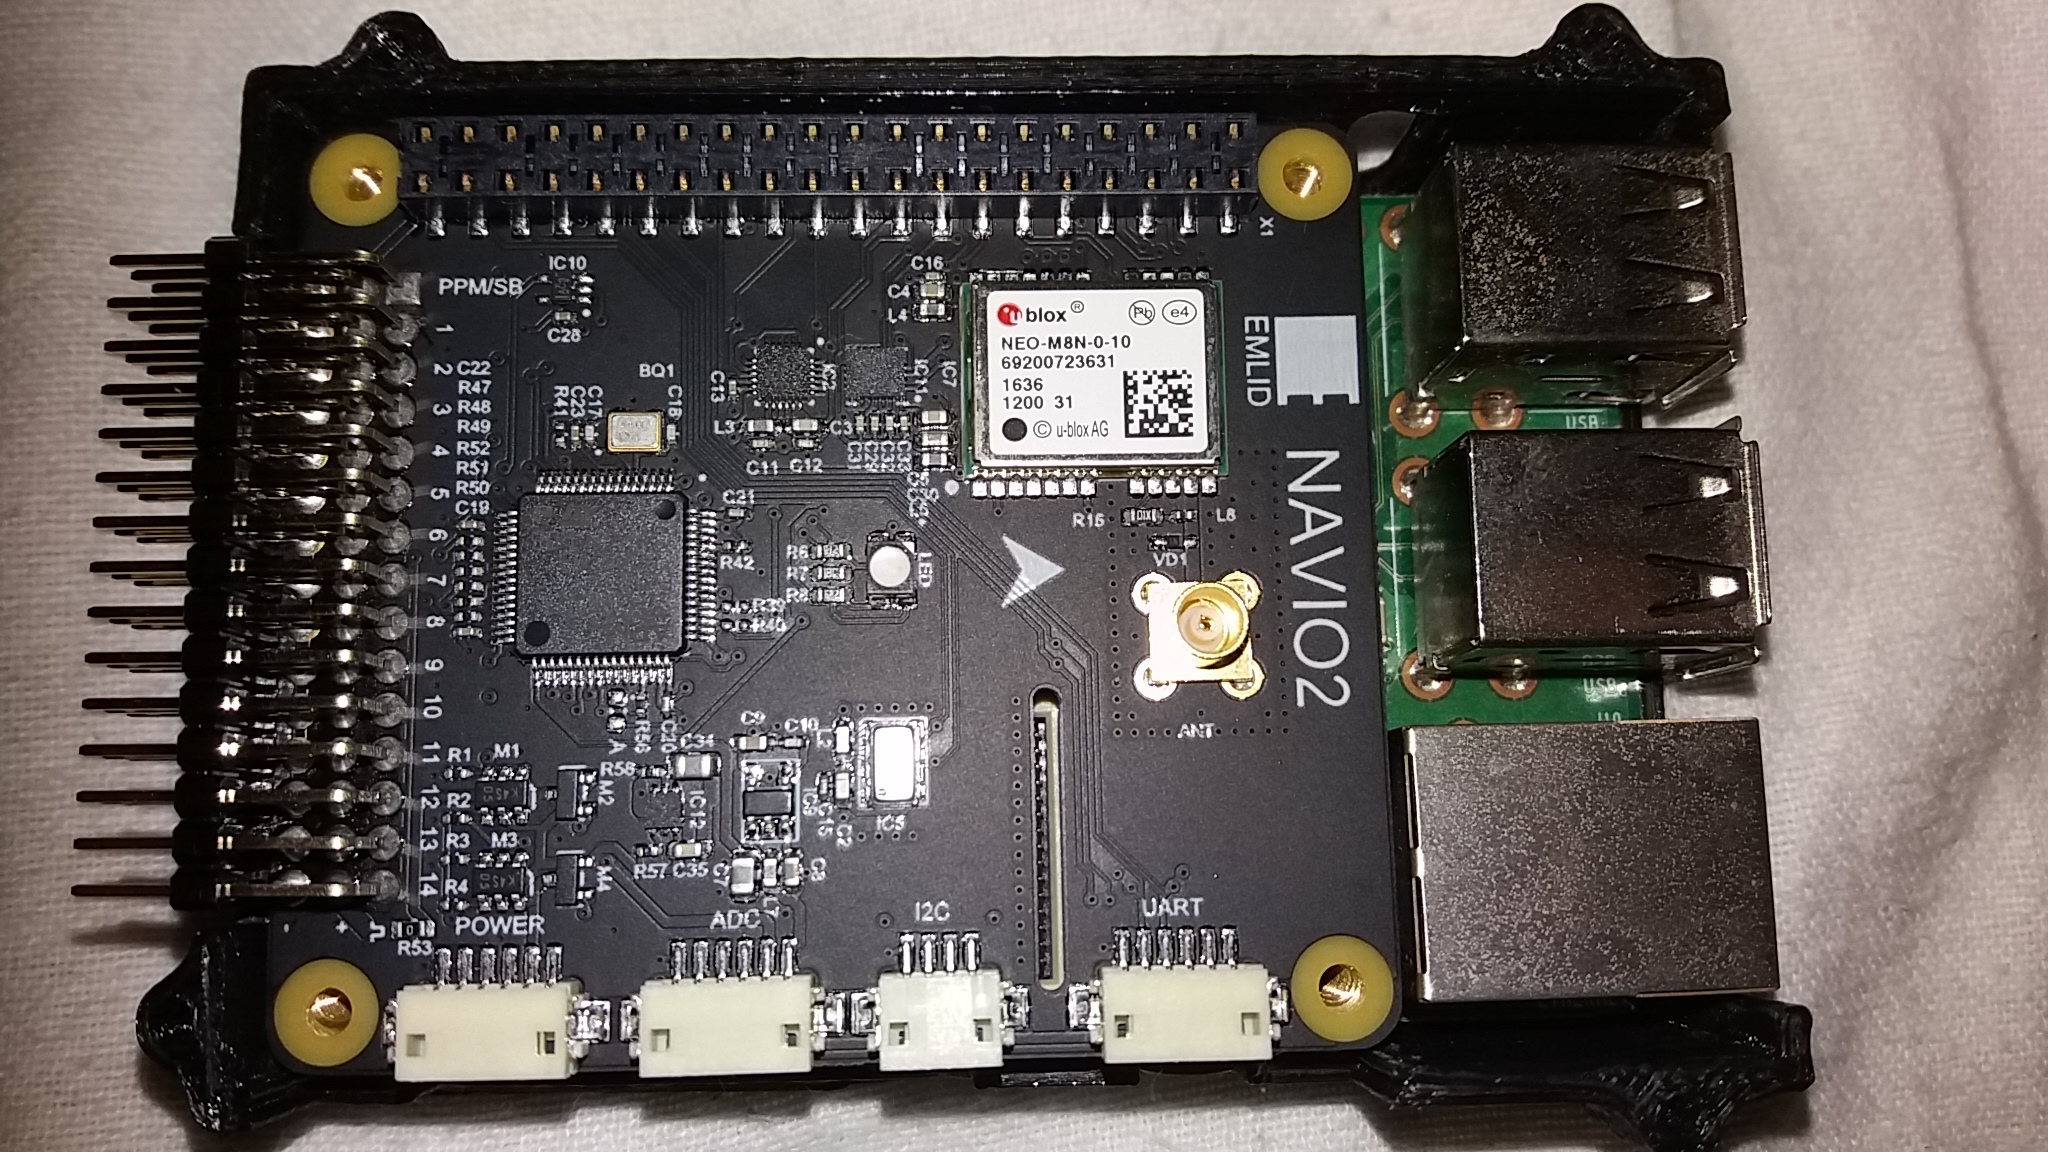
\includegraphics[scale=0.1]{images/drone-build-3dcase-pi-navio.jpg}
\caption{Fitting the Navio2 flight controller on top.}
\label{fig:insertion_navio}
\end{subfigure}
\caption{Inserting the sensitive electronics.}
\label{fig:insertion}
\end{figure}

\begin{figure}[H]
\begin{subfigure}{0.5\textwidth}
\centering
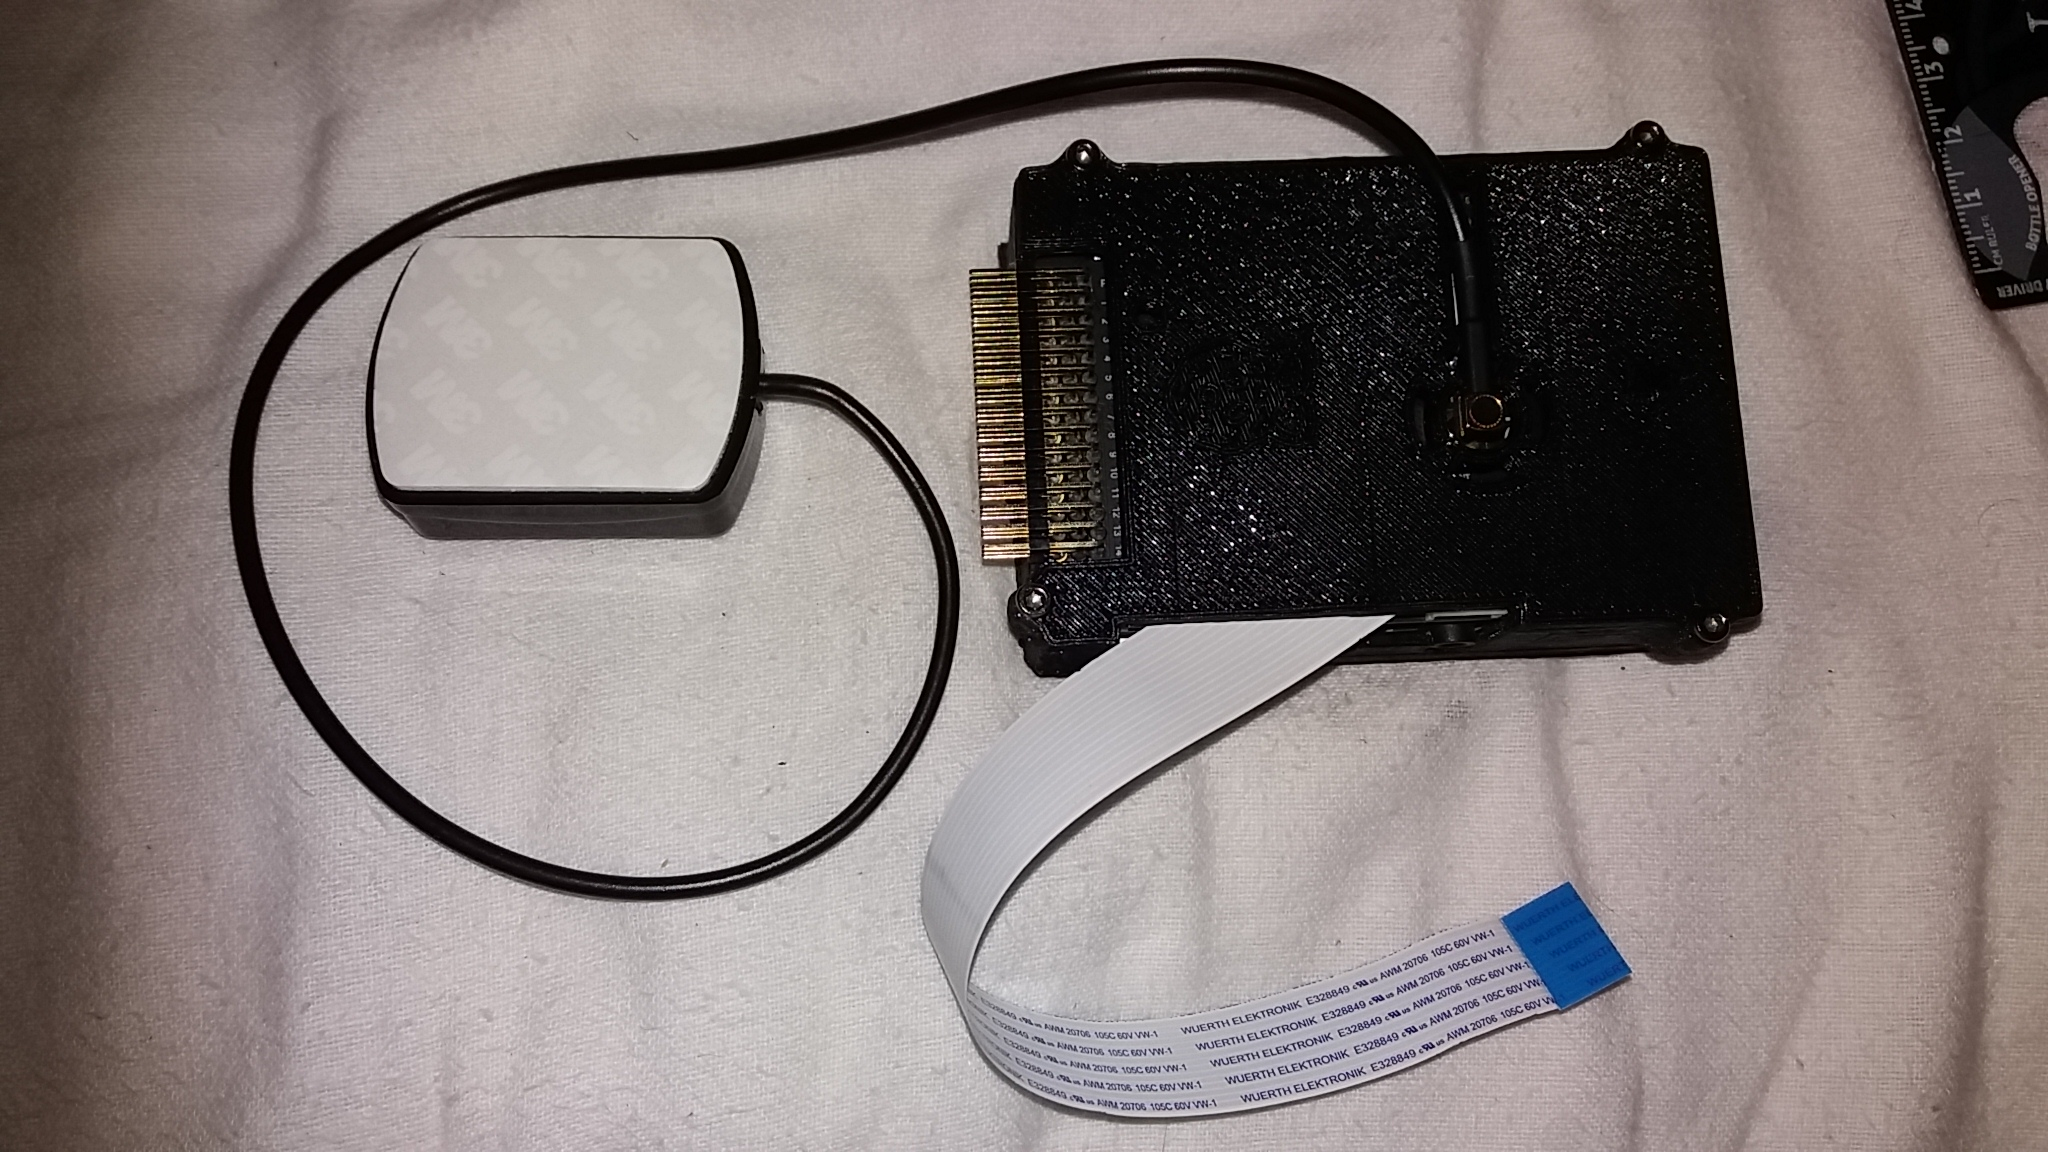
\includegraphics[scale=0.1]{images/drone-build-3dcase-gps.jpg}
\caption{Connecting Ublox Neo-7 GPS antenna and 15-pin camera CSI ribbon cable.}
\label{fig:stab_gps}
\end{subfigure}
\begin{subfigure}{0.5\textwidth}
\centering
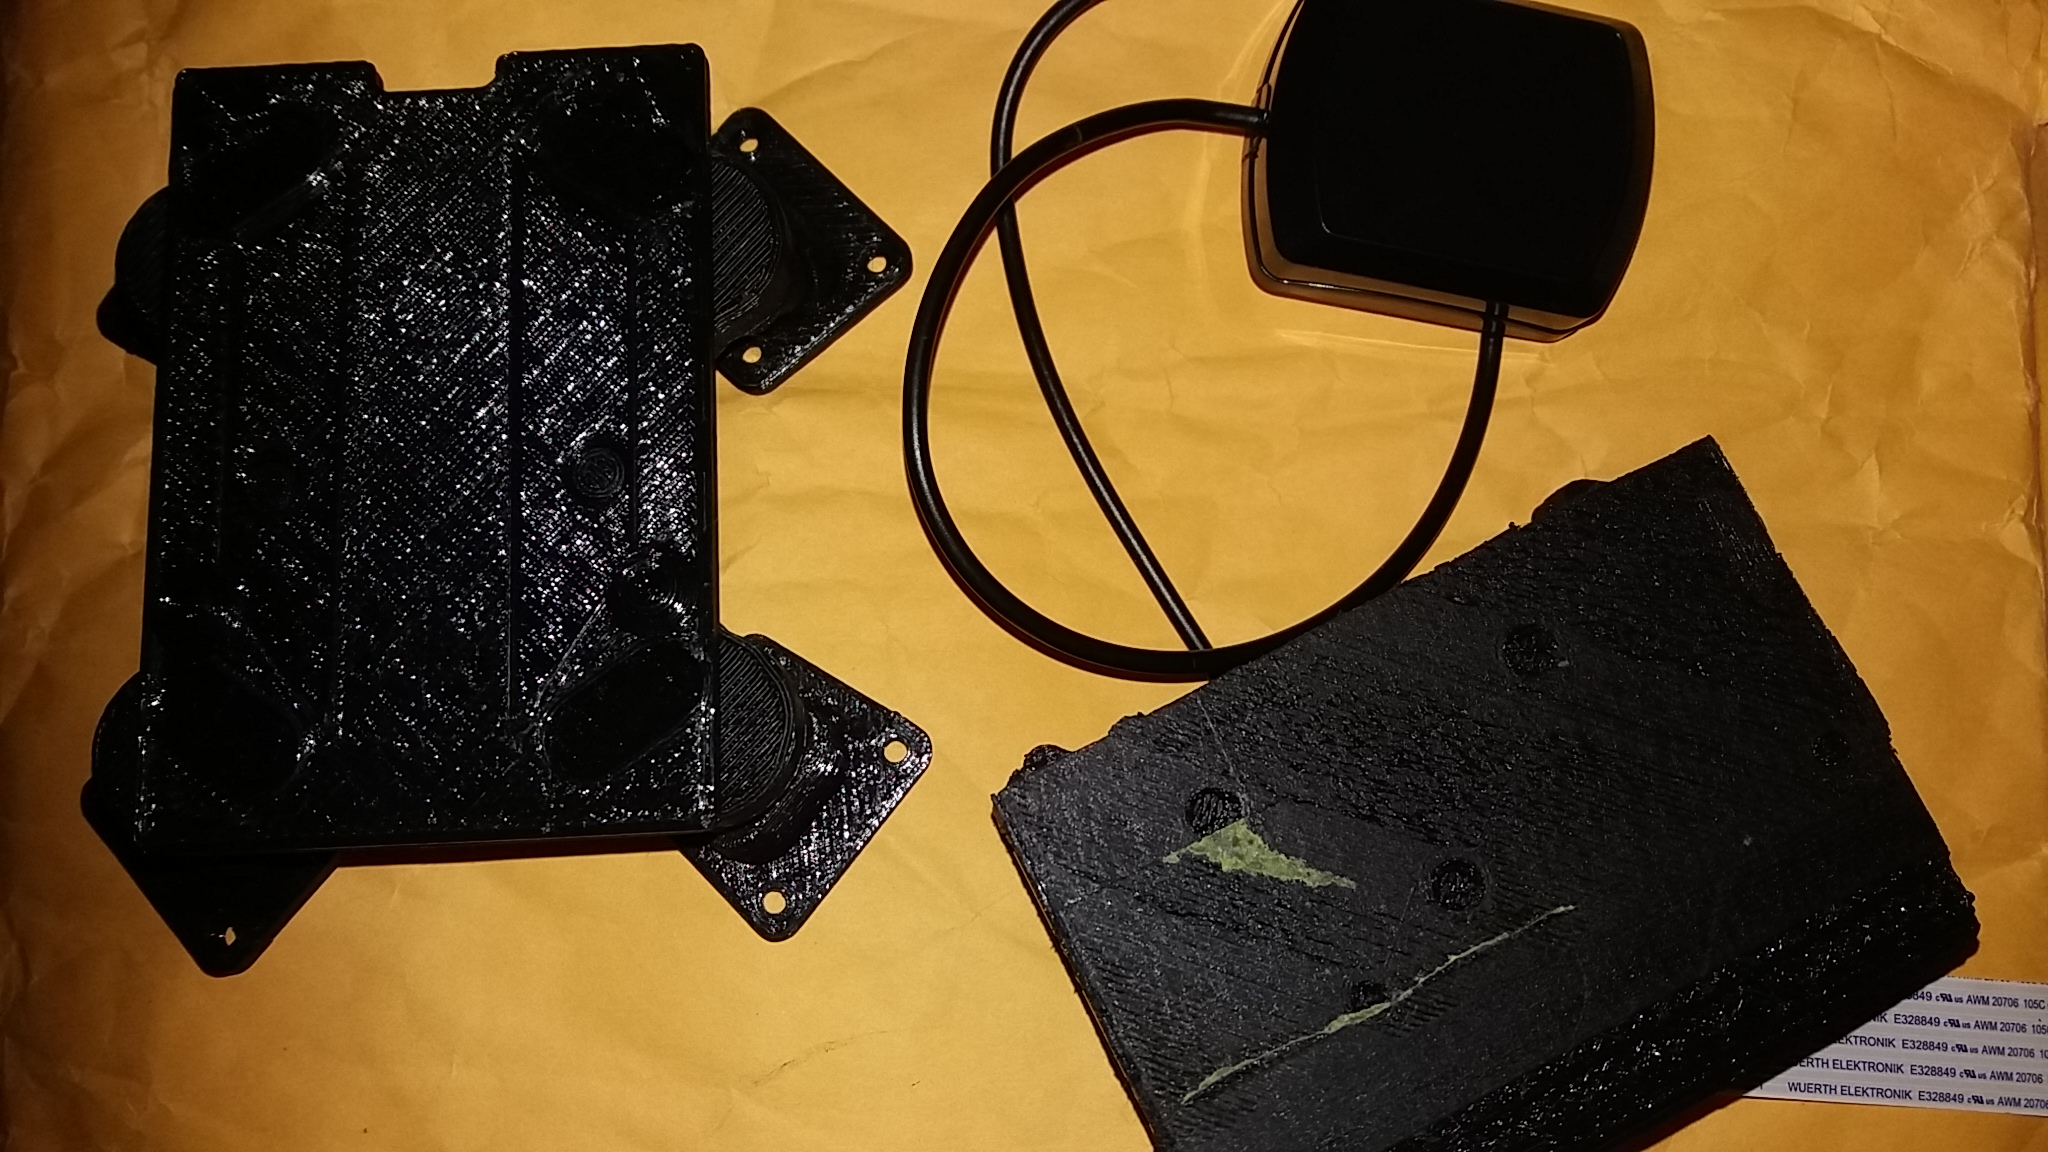
\includegraphics[scale=0.1]{images/drone-build-3dplatform.jpg}
\caption{Case and platform}
\label{fig:stab_case_plat}
\end{subfigure}
\caption{Putting the case and platform together}
\label{fig:stabilize_platform}
\end{figure}

The GPS antenna lead fits snugly onto an SMA connector in Figure \ref{fig:stab_gps}, and is exposed in such a way as to leave enough freedom for the cable to bend, but not wear as if it were rigidly attached.

\begin{figure}[H]
\begin{subfigure}{0.5\textwidth}
\centering
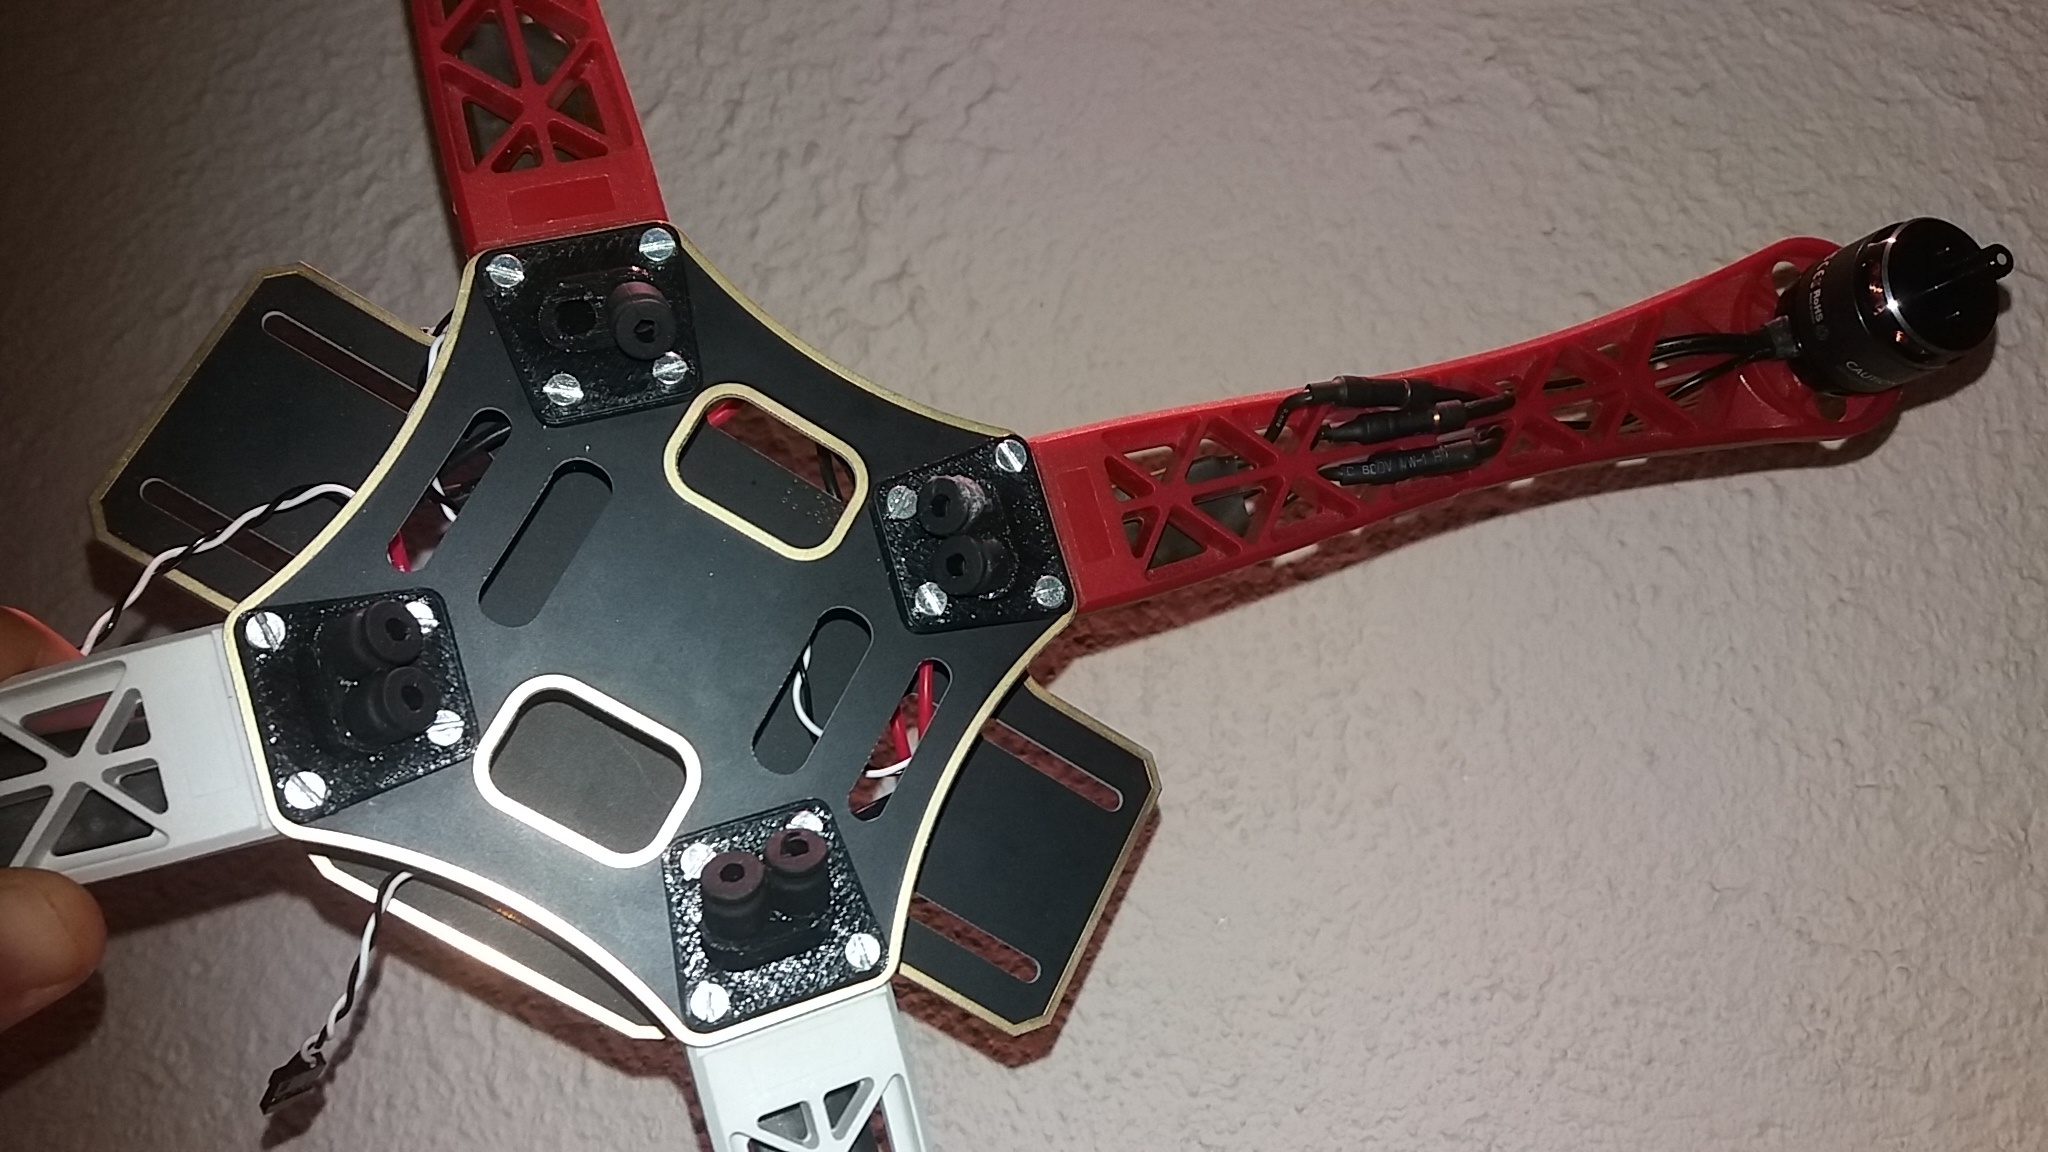
\includegraphics[scale=0.1]{images/drone-build-feet.jpg}
\caption{Added feet for platform.} 
\label{fig:feet}
\end{subfigure}
\begin{subfigure}{0.5\textwidth}
\centering
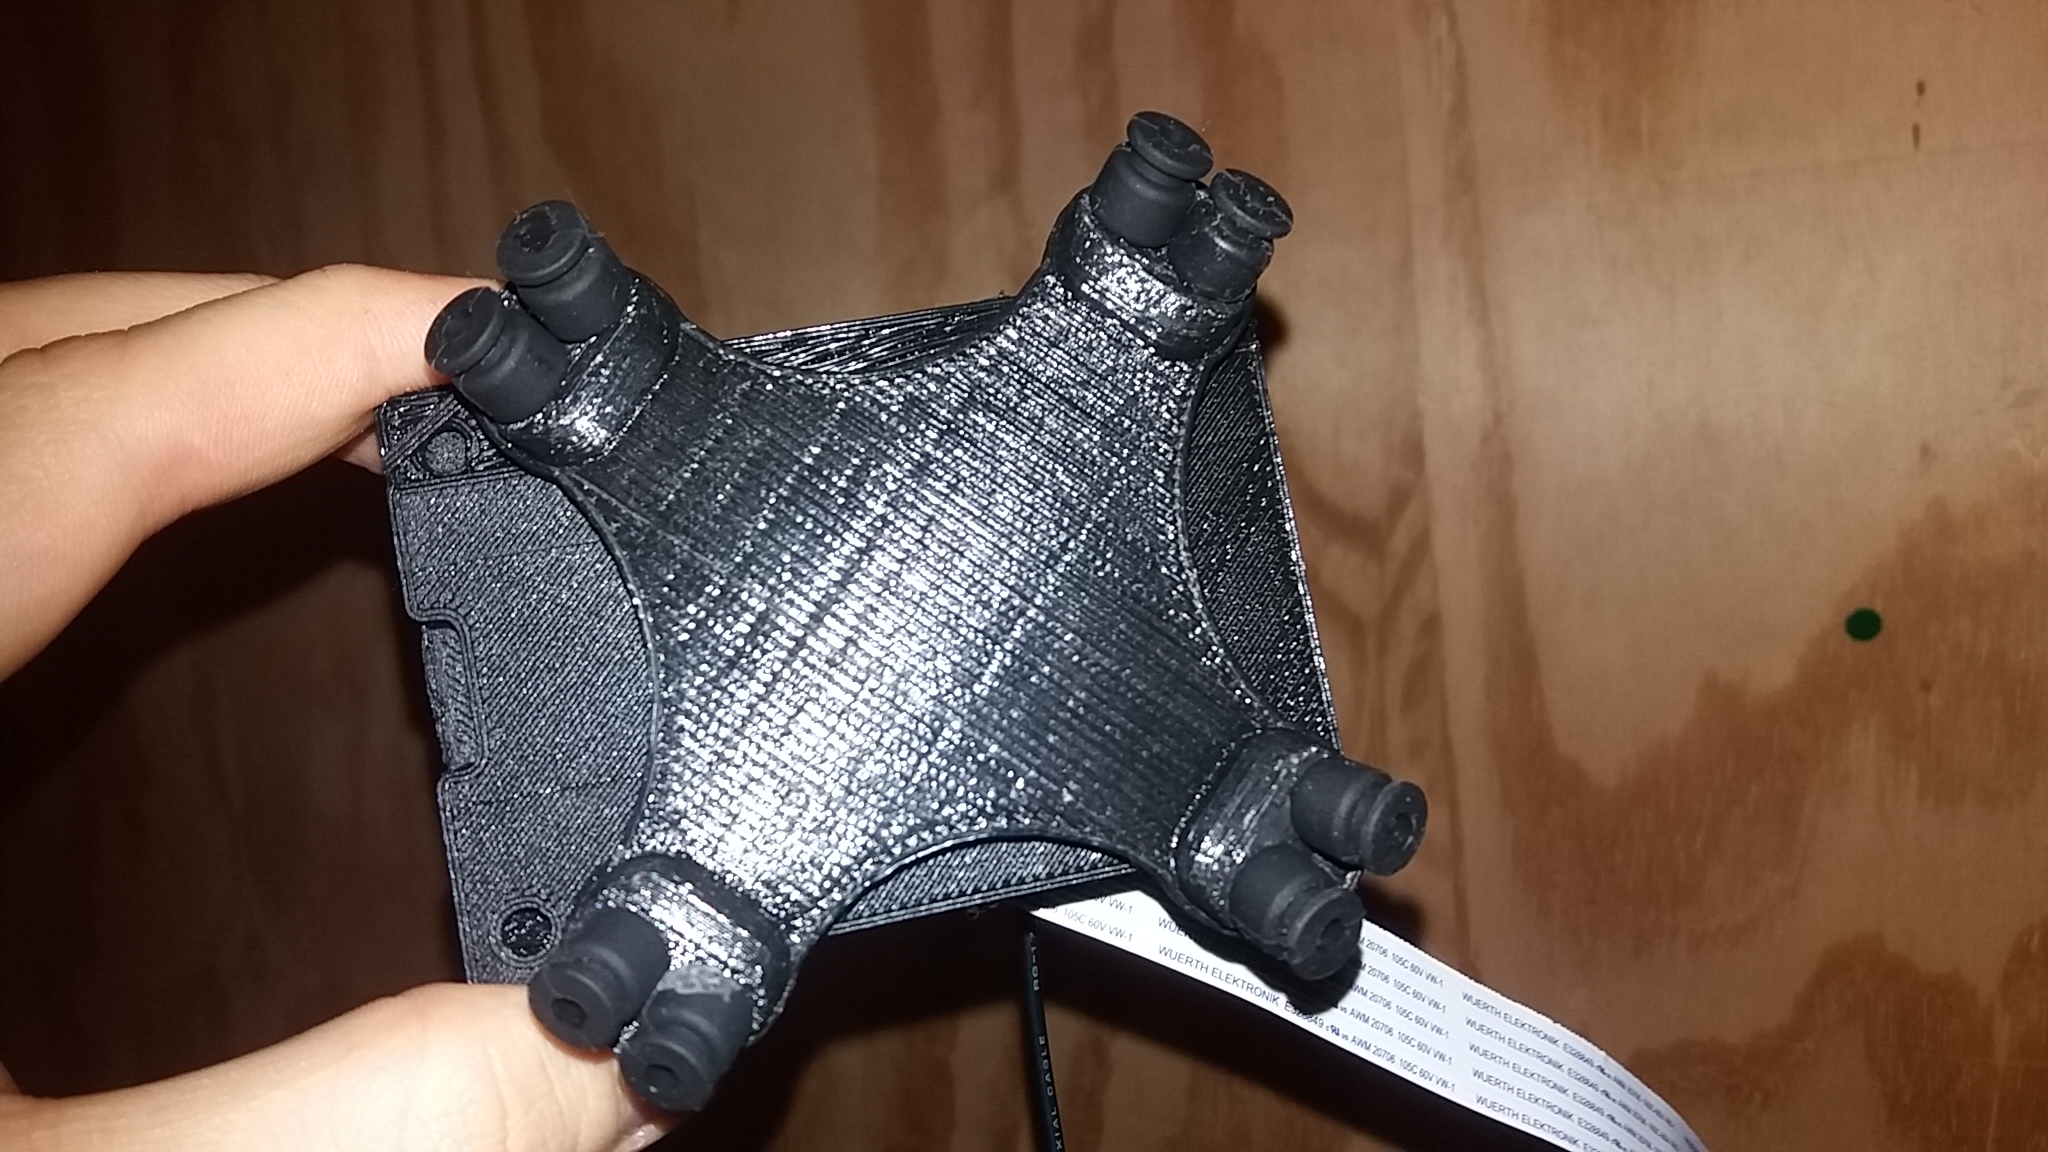
\includegraphics[scale=0.1]{images/drone-build-damper-balls.jpg}
\caption{Rubber vibration damper balls for platform.}
\label{fig:balls}
\end{subfigure}
\caption{Isolating vibrations between flight controller and the rest of the drone}
\label{fig:stabilize_platform}
\end{figure}

One of the biggest problems in a drone is the vibrations emanating from the motors, travelling along the frame and affecting the flight controller. If not isolated from the flight controller, they induce a disturbance to the PID loop since the accuracy of the gyroscope, accelerometer and barometer readings are affected. In some cases, disturbed more than the PID loop can reasonably determine the current state of the drone.\\

Thus, damper balls can be used to isolate vibrations significantly from the flight controller.

\begin{figure}[H]
\begin{subfigure}{0.5\textwidth}
\centering
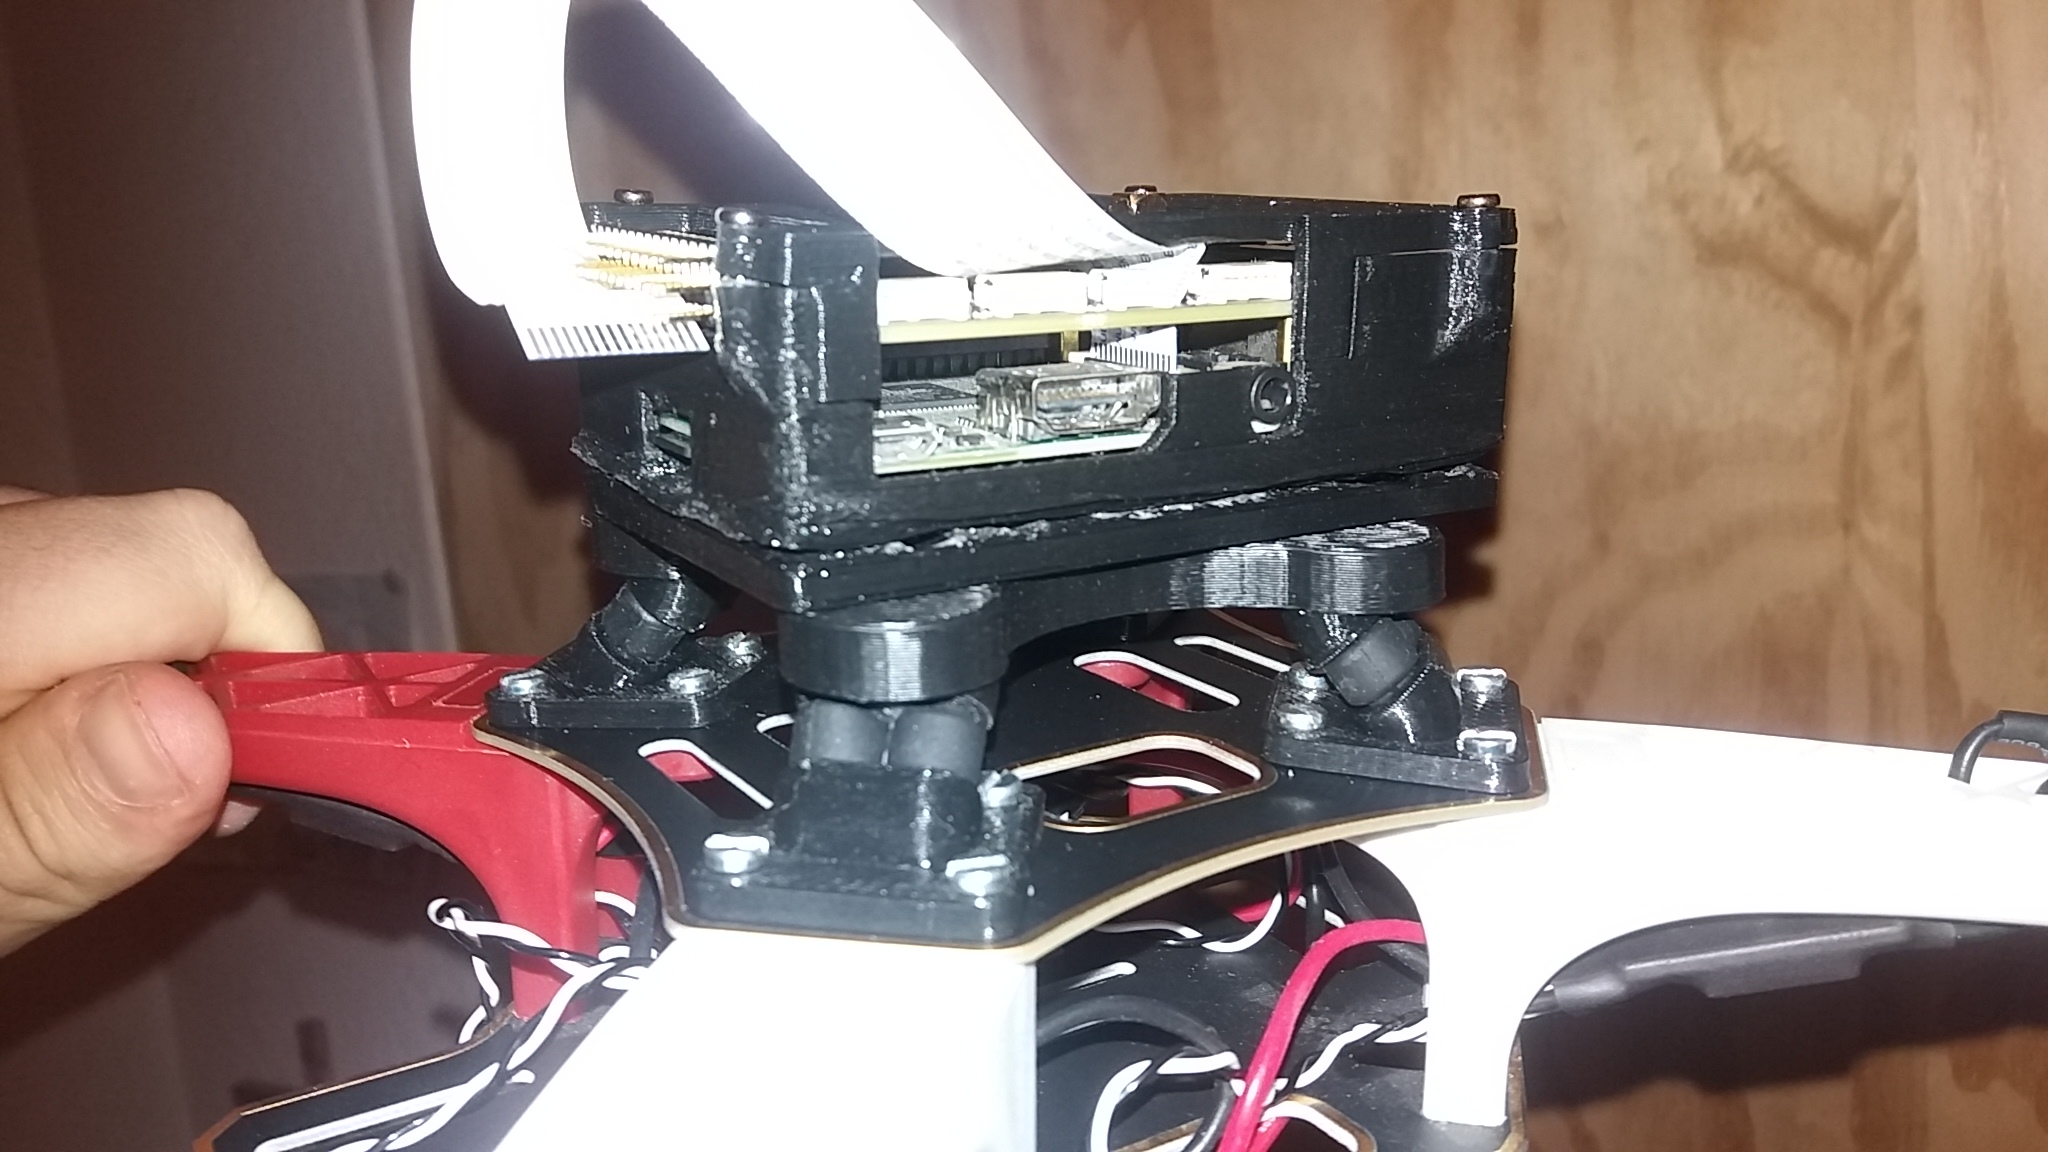
\includegraphics[scale=0.1]{images/drone-build-case-ondrone.jpg}
\caption{Attaching 3D printed case and platform to drone.}
\label{fig:attach_case_drone}
\end{subfigure}
\begin{subfigure}{0.5\textwidth}
\centering
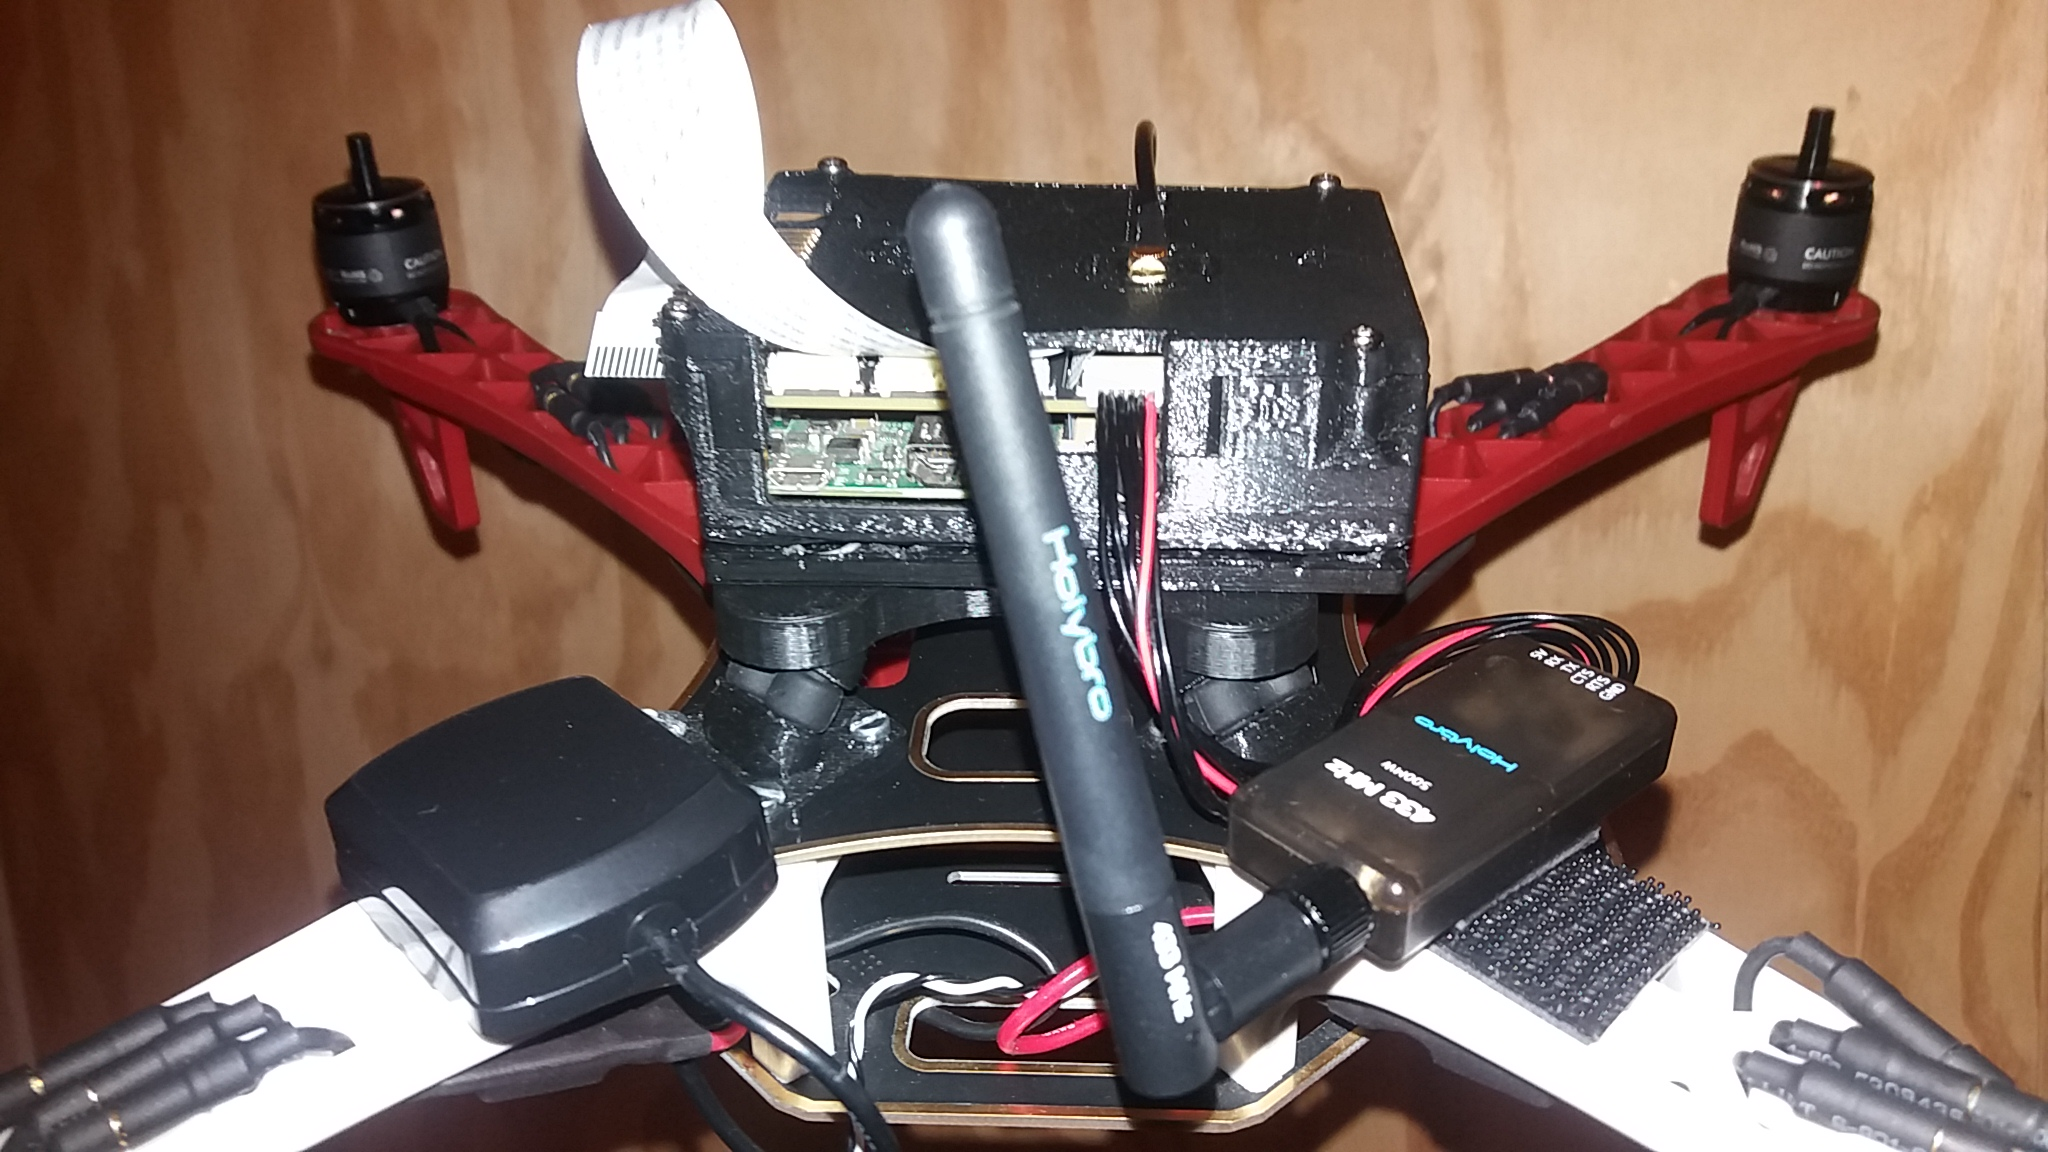
\includegraphics[scale=0.1]{images/drone-build-433.jpg}
\caption{Adding 433MHz telemtery to drone.}
\label{fig:attach_433}
\end{subfigure}
\caption{Isolating vibrations between flight controller and the rest of the drone}
\label{fig:attach_case_433}
\end{figure}

\begin{figure}[H]
\begin{subfigure}{0.5\textwidth}
\centering
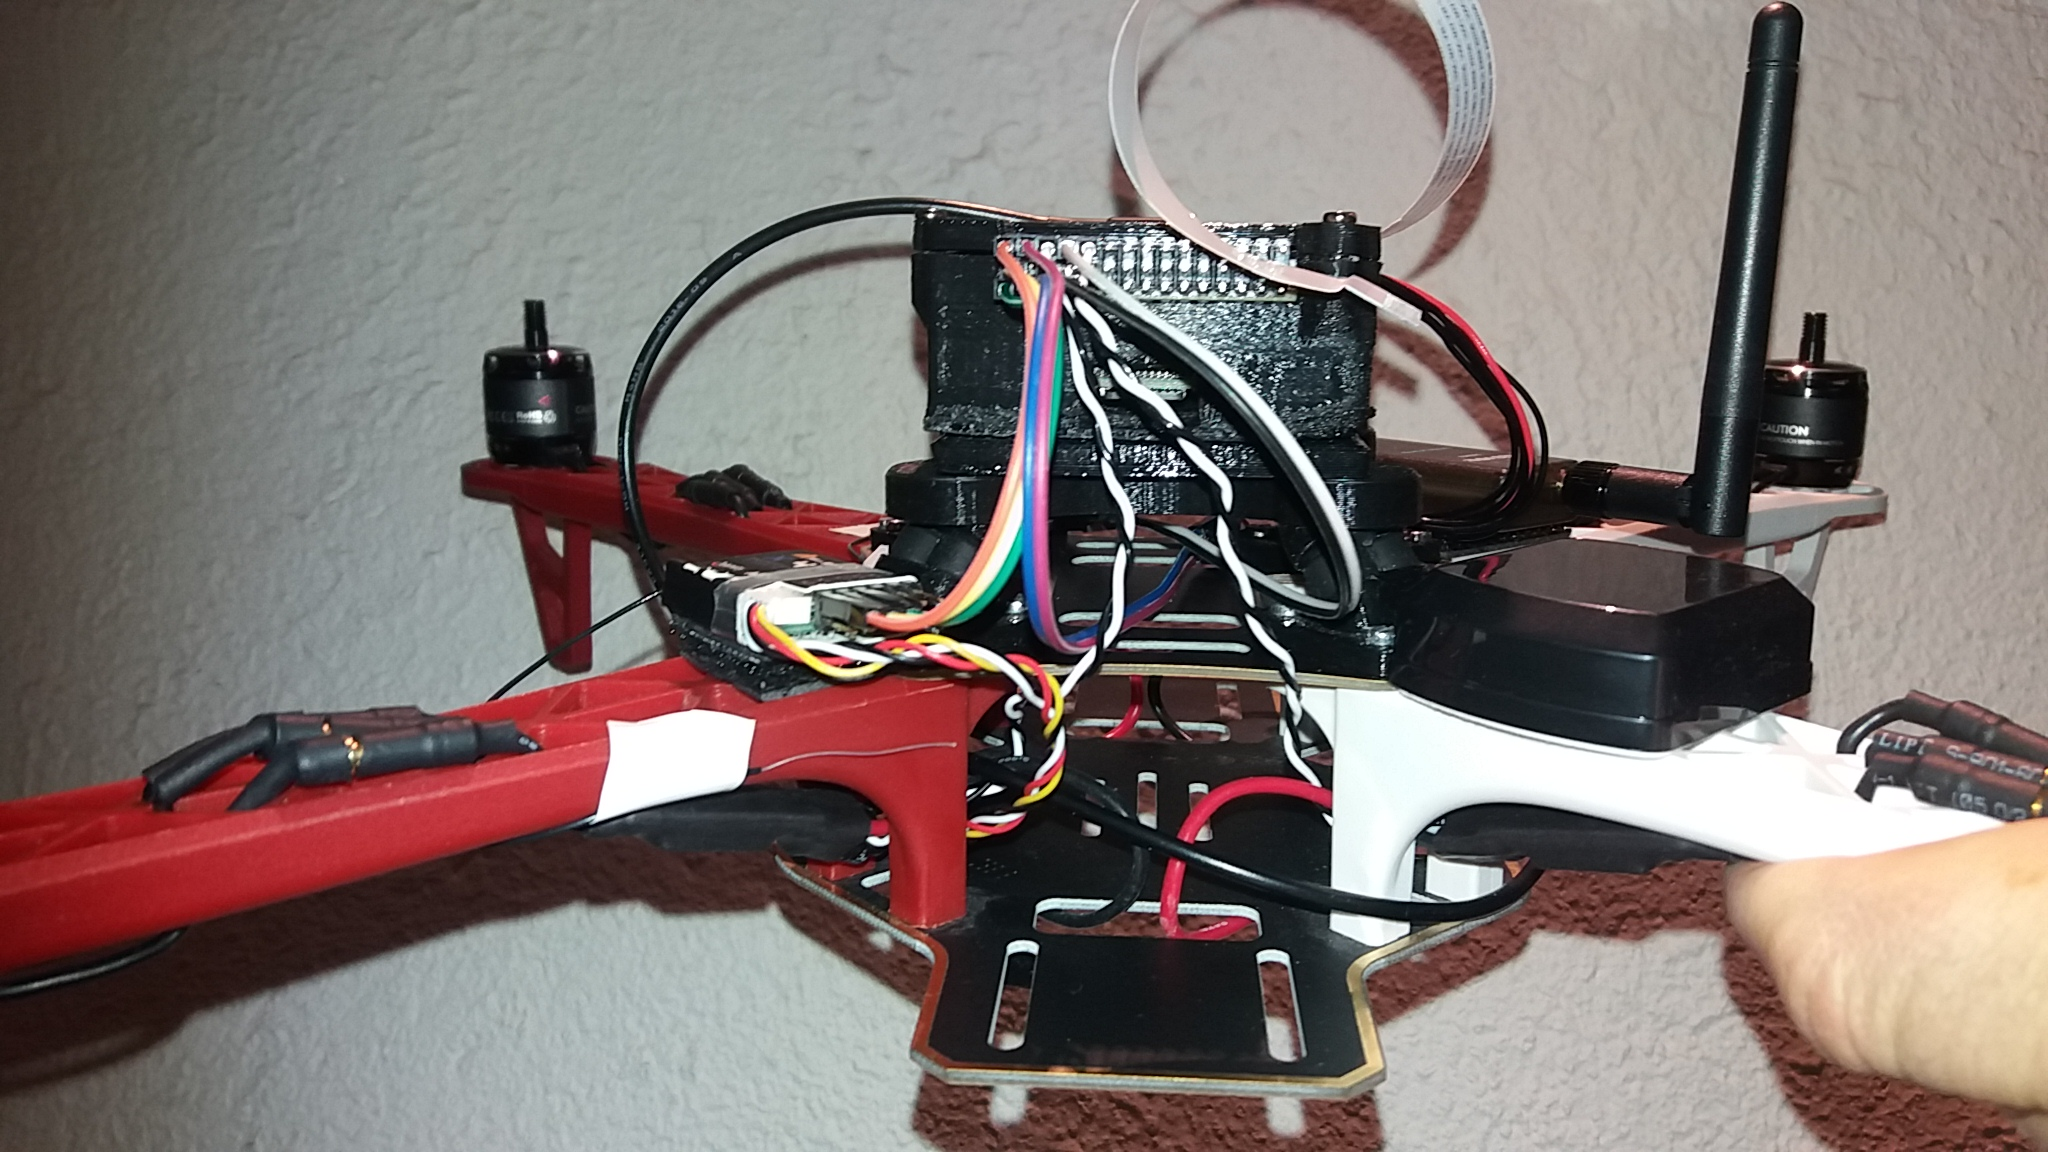
\includegraphics[scale=0.1]{images/drone-build-signal-wires.jpg}
\caption{Wiring up the signal wires}
\label{fig:attach_sbus}
\end{subfigure}
\begin{subfigure}{0.5\textwidth}
\centering
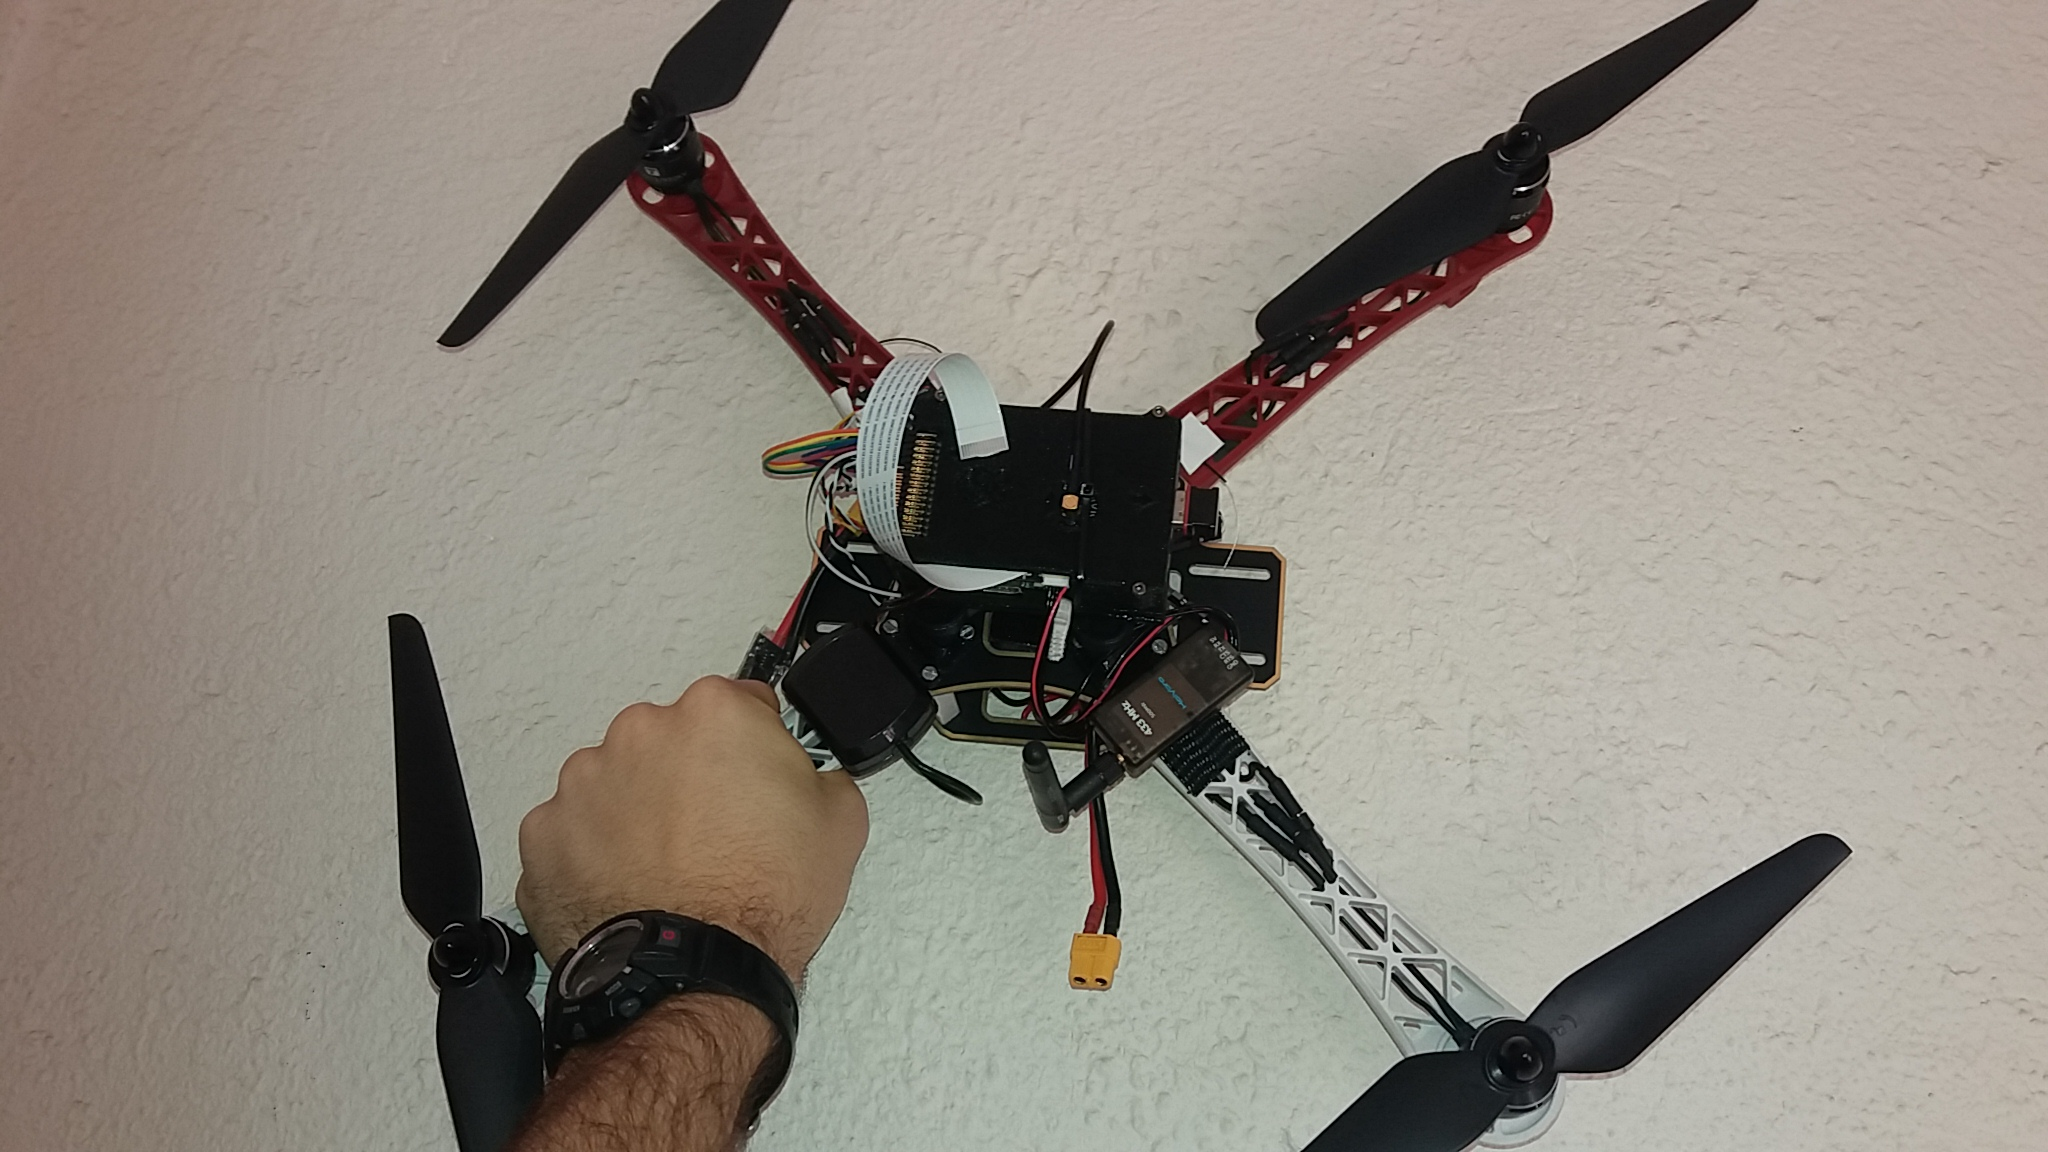
\includegraphics[scale=0.1]{images/drone-build-props.jpg}
\caption{Adding the 9.5'x4.5' propellers}
\label{fig:attach_props}
\end{subfigure}
\caption{Ready to fly}
\label{fig:attach_signal_props}
\end{figure}

\section{Ground Control Station}

The GCS is necessary for pre-flight checks, monitoring/controlling the status of the vehicle during flight, and setting waypoints.\\

The drone communicates with the GCS in Figure \ref{fig:gcs} using 433 MHz transceivers as in Figure \ref{fig:attach_433}.

\begin{figure}[H]
\centering
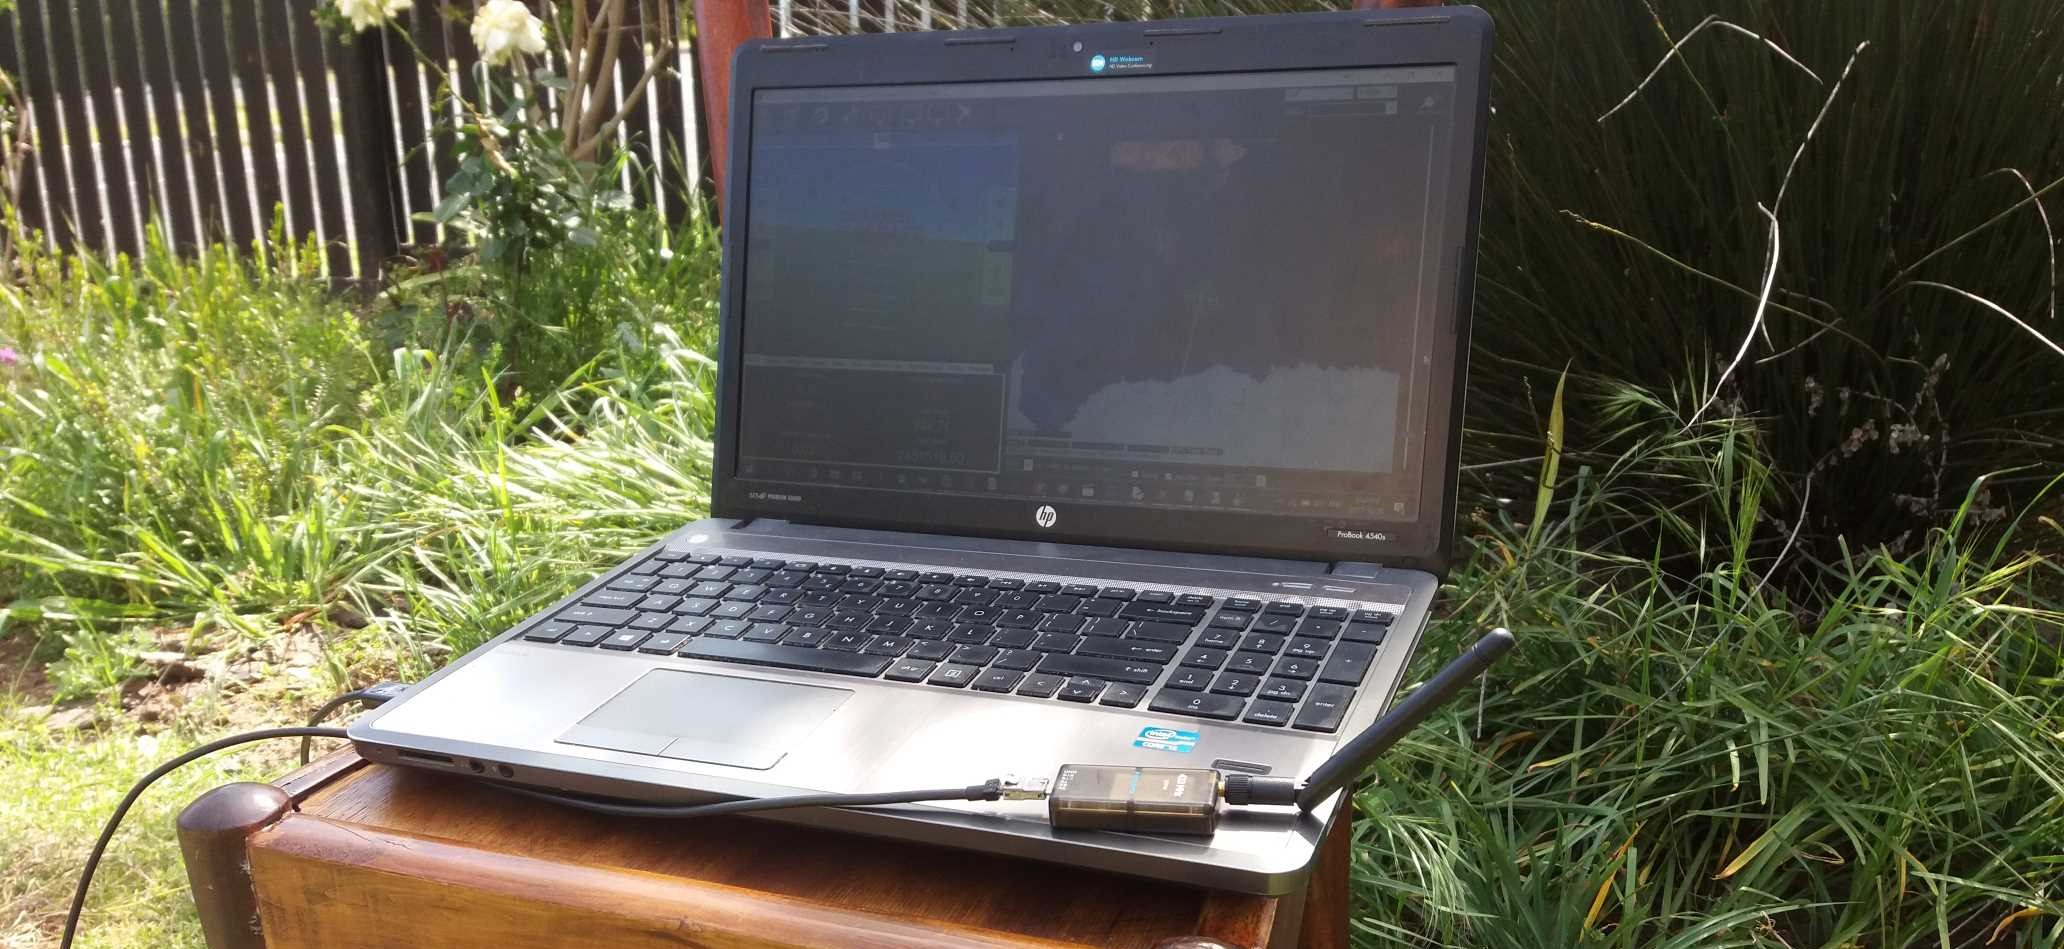
\includegraphics[scale=0.17]{images/gcs.jpg}
\caption{Ground Control Station}
\label{fig:gcs}
\end{figure}

The software used is the open source Mission Planner platform.

\begin{figure}[H]
\centering
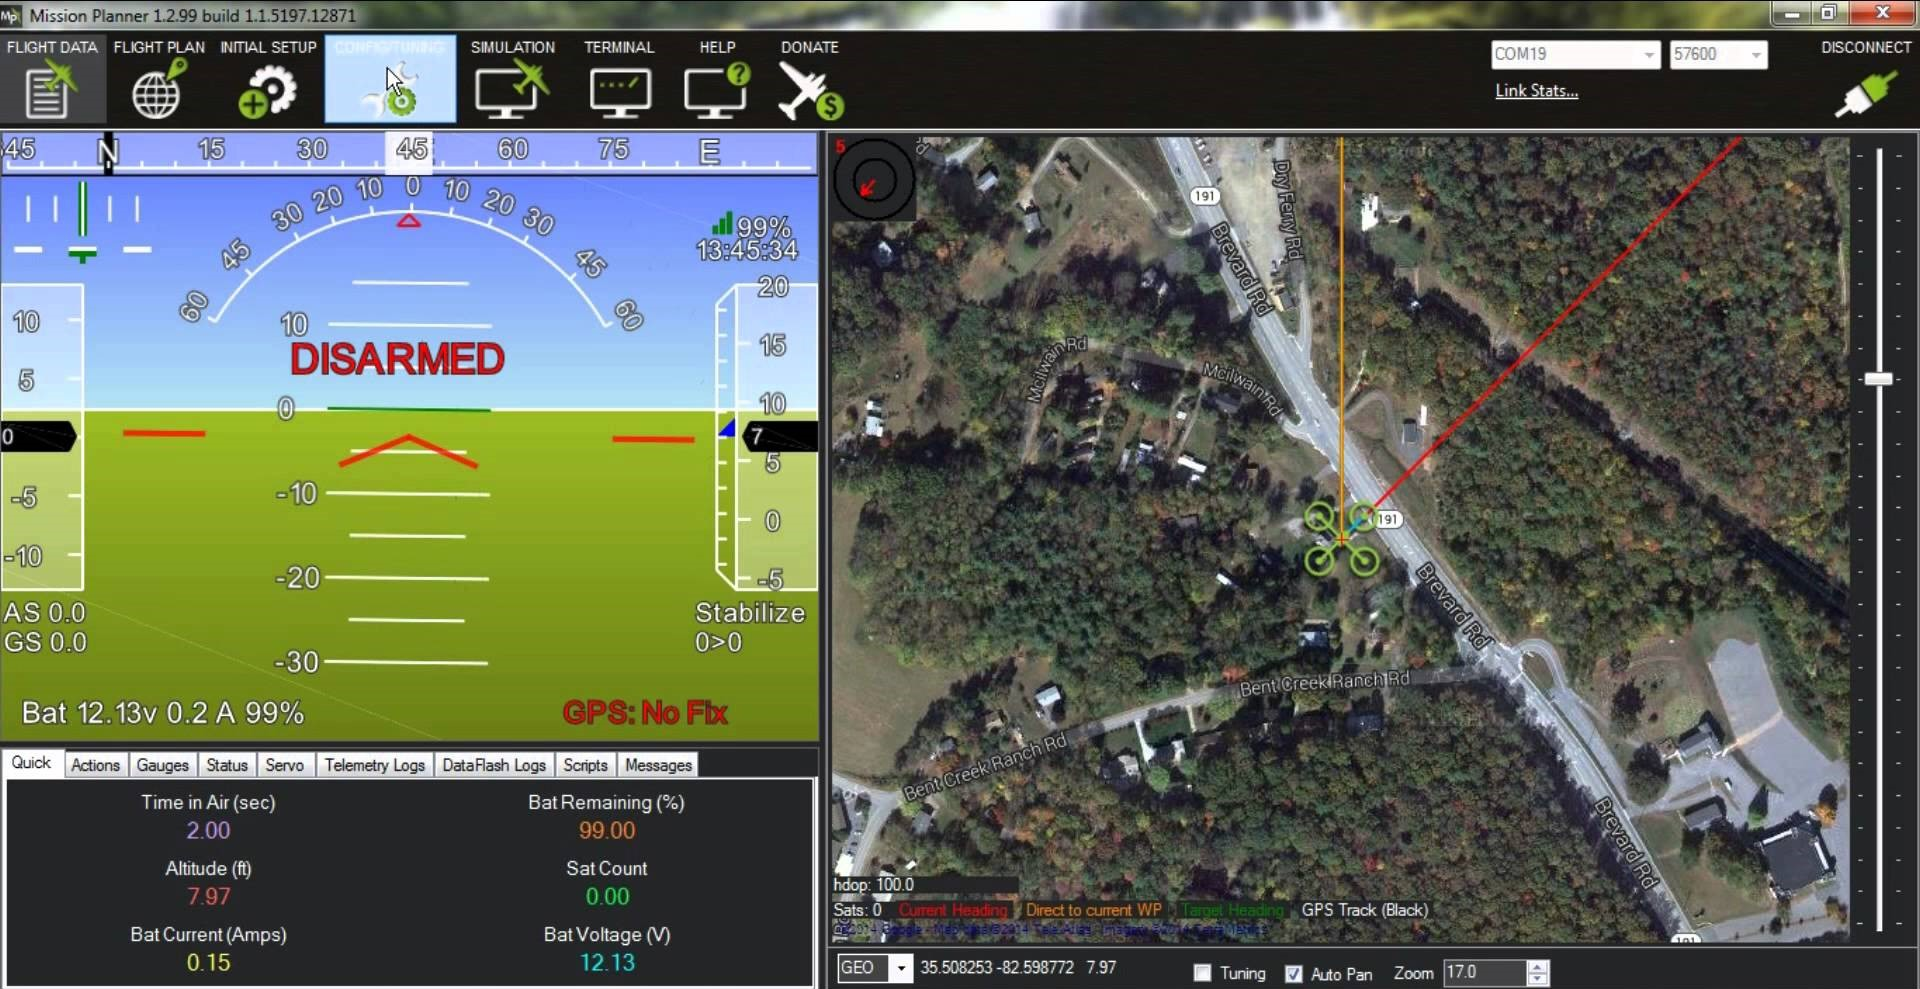
\includegraphics[scale=0.2]{images/mp.jpg}
\caption{Mission planner}
\label{fig:mission_planner}
\end{figure}

\section{Remote controller}
\label{sec:remote_controller}

The remote controller is used to manually control the drone. It is also used to monitor the battery and signal strength.\\

\begin{figure}[H]
\begin{subfigure}{0.5\textwidth}
\centering
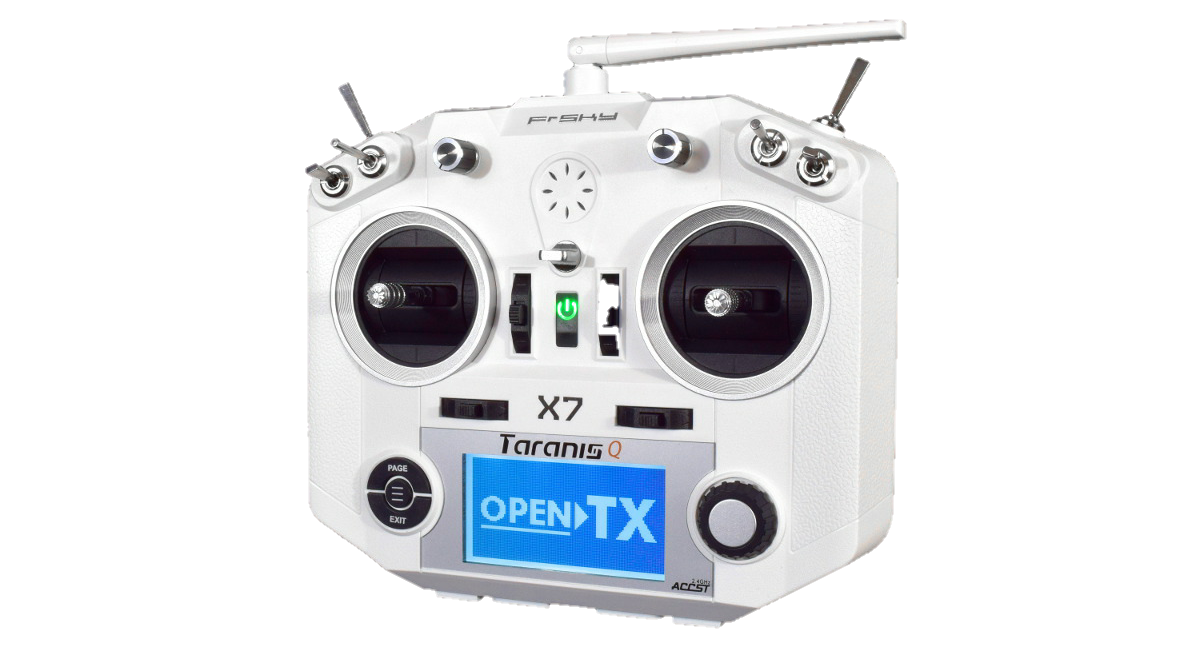
\includegraphics[scale=0.255]{images/taranis.png}
\caption{Taranis Q X7 remote controller}
\label{fig:remote_controller}
\end{subfigure}
\begin{subfigure}{0.5\textwidth}
\centering
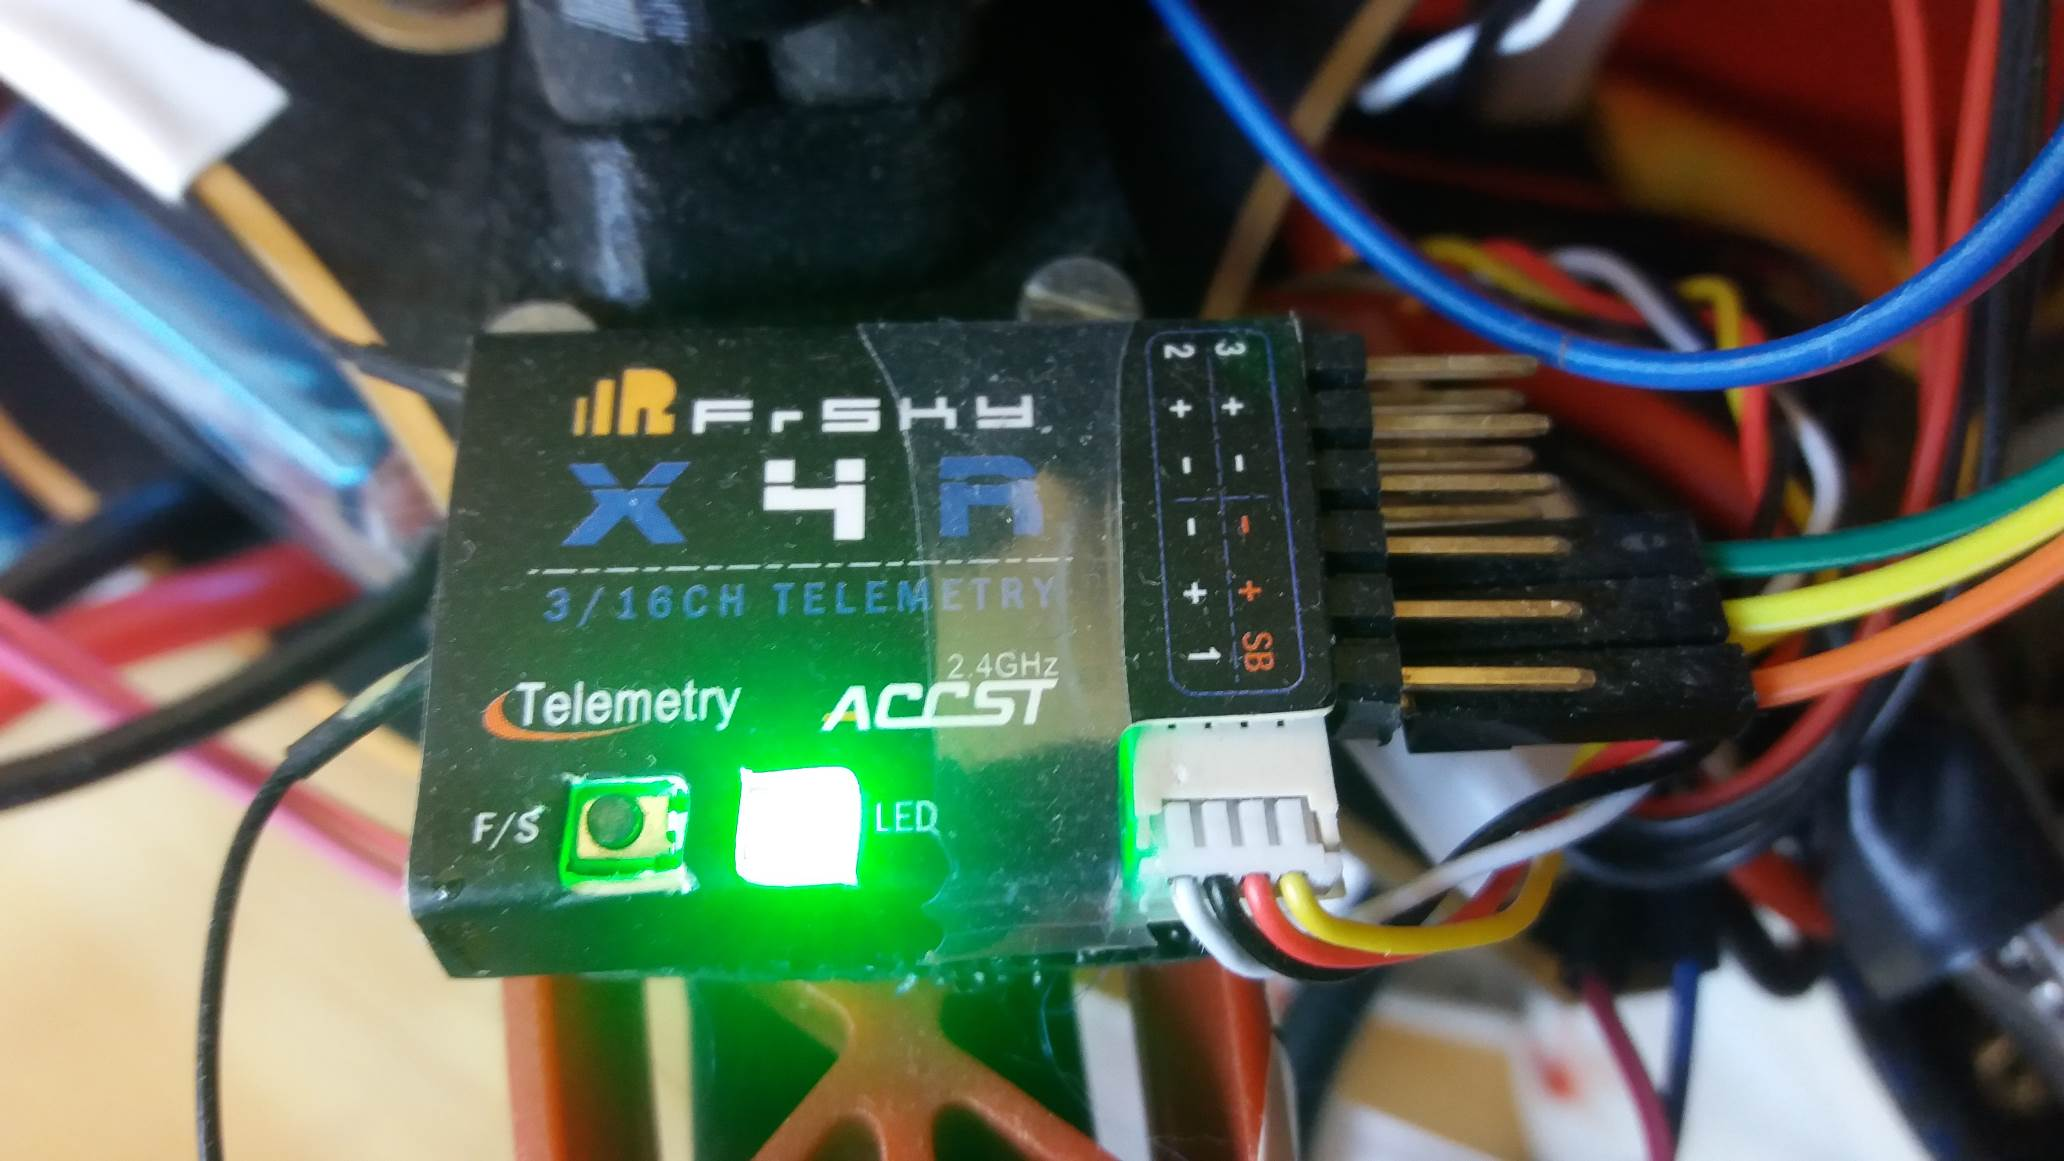
\includegraphics[scale=0.15]{images/frsky_transceiver.jpg}
\caption{FrSky X4R transceiver}
\label{fig:balls}
\end{subfigure}
\caption{Remote controller and on-board transceiver}
\label{fig:frsky_transceiver}
\end{figure}

The full-duplex remote controller outputs at 100mW. The FrSky X4R transceiver has two antennae, and also outputs at 100 mW.\\

At first, the Taranis remote controller is bound to the FrSky X4R transceiver aboard the drone in Figure \ref{fig:frsky_transceiver}. This is done by holding in the `F\/S' button on the transceiver while powering it on, and entering bind mode on the remote controller.

\begin{figure}[H]
\begin{subfigure}{0.5\textwidth}
\centering
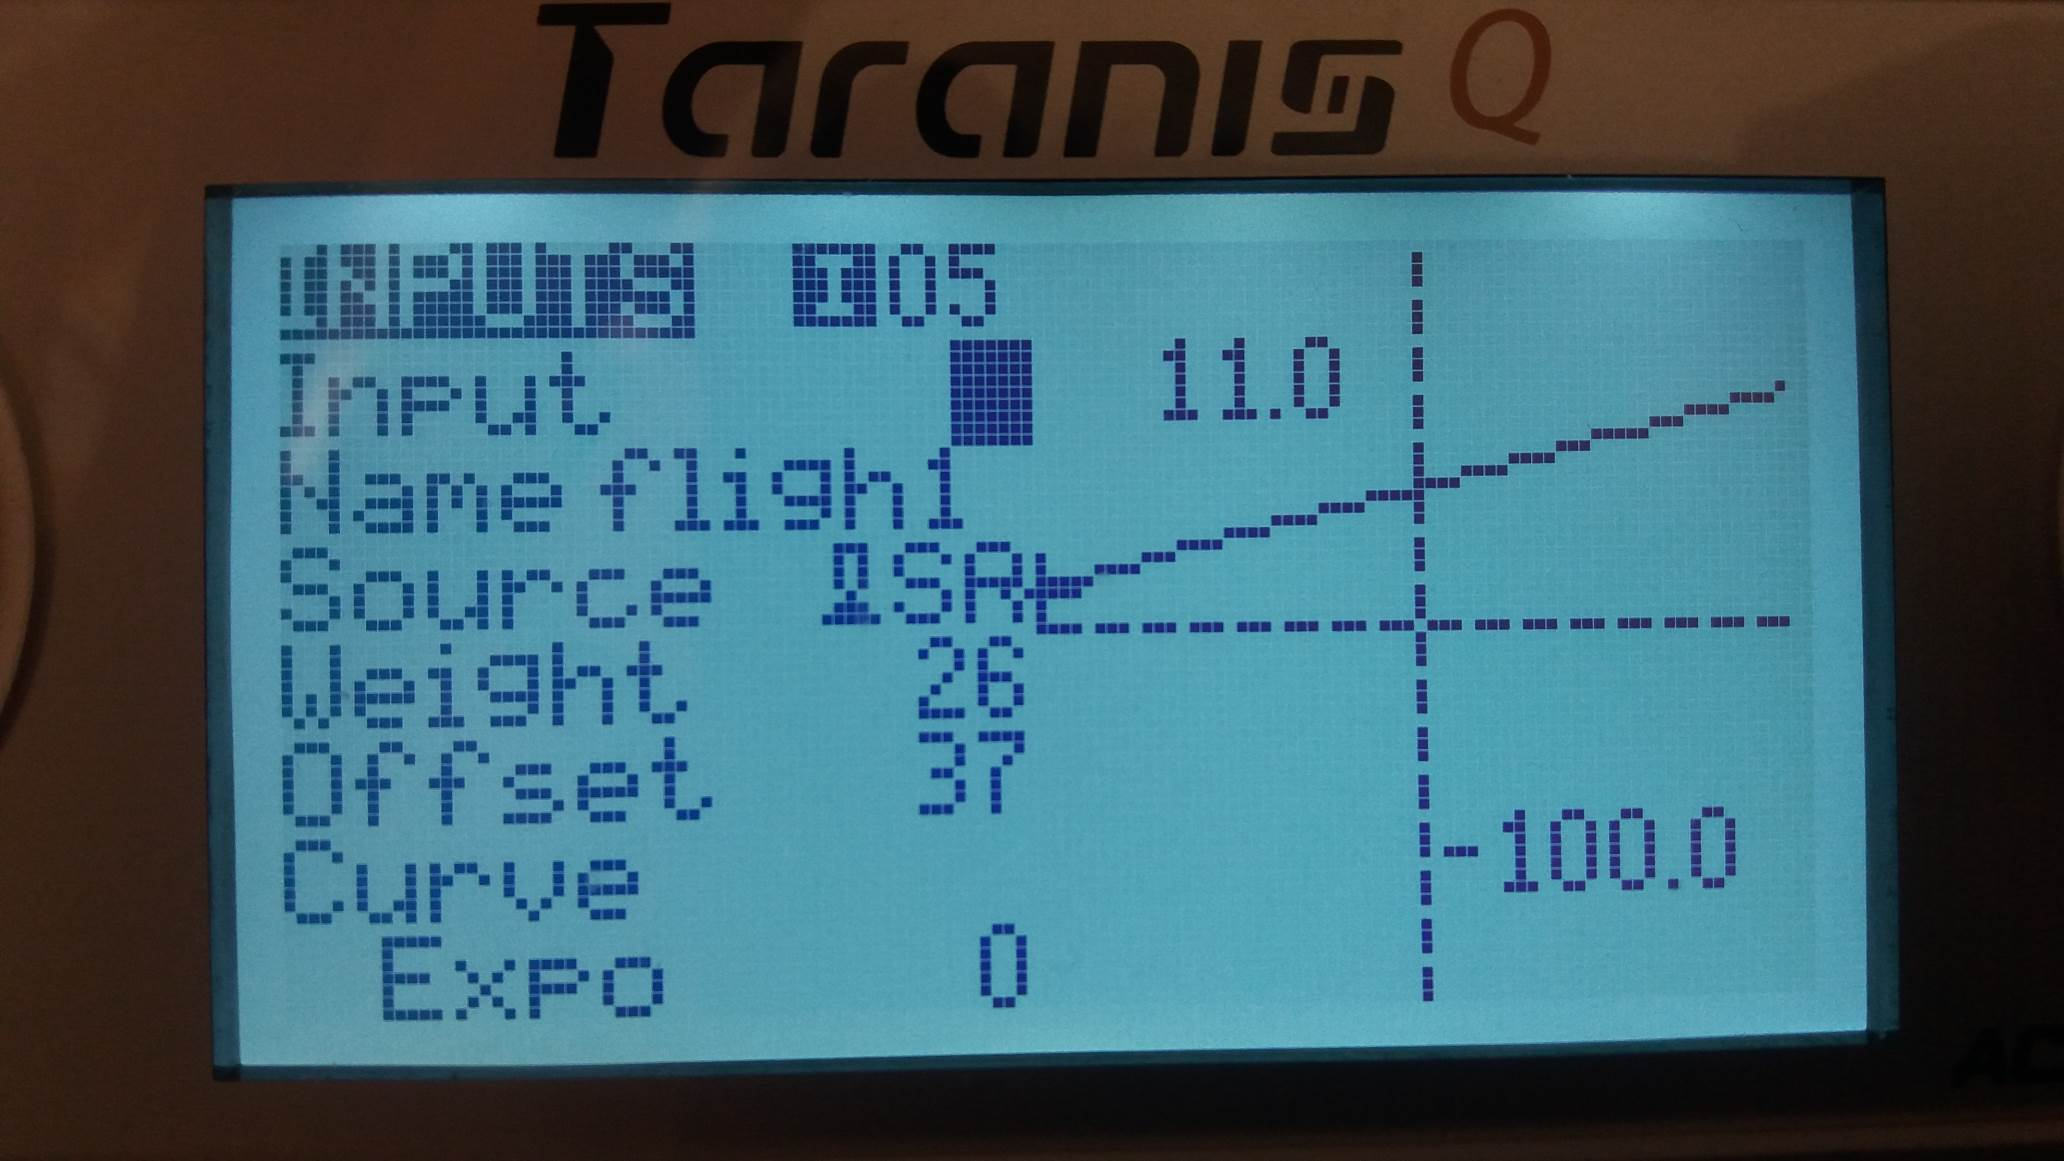
\includegraphics[scale=0.13]{images/lcd/flight_mode_but_1.jpg}
\caption{Linearised flight mode switch 1 input}
\label{fig:taranis_fm_but1}
\end{subfigure}
\begin{subfigure}{0.5\textwidth}
\centering
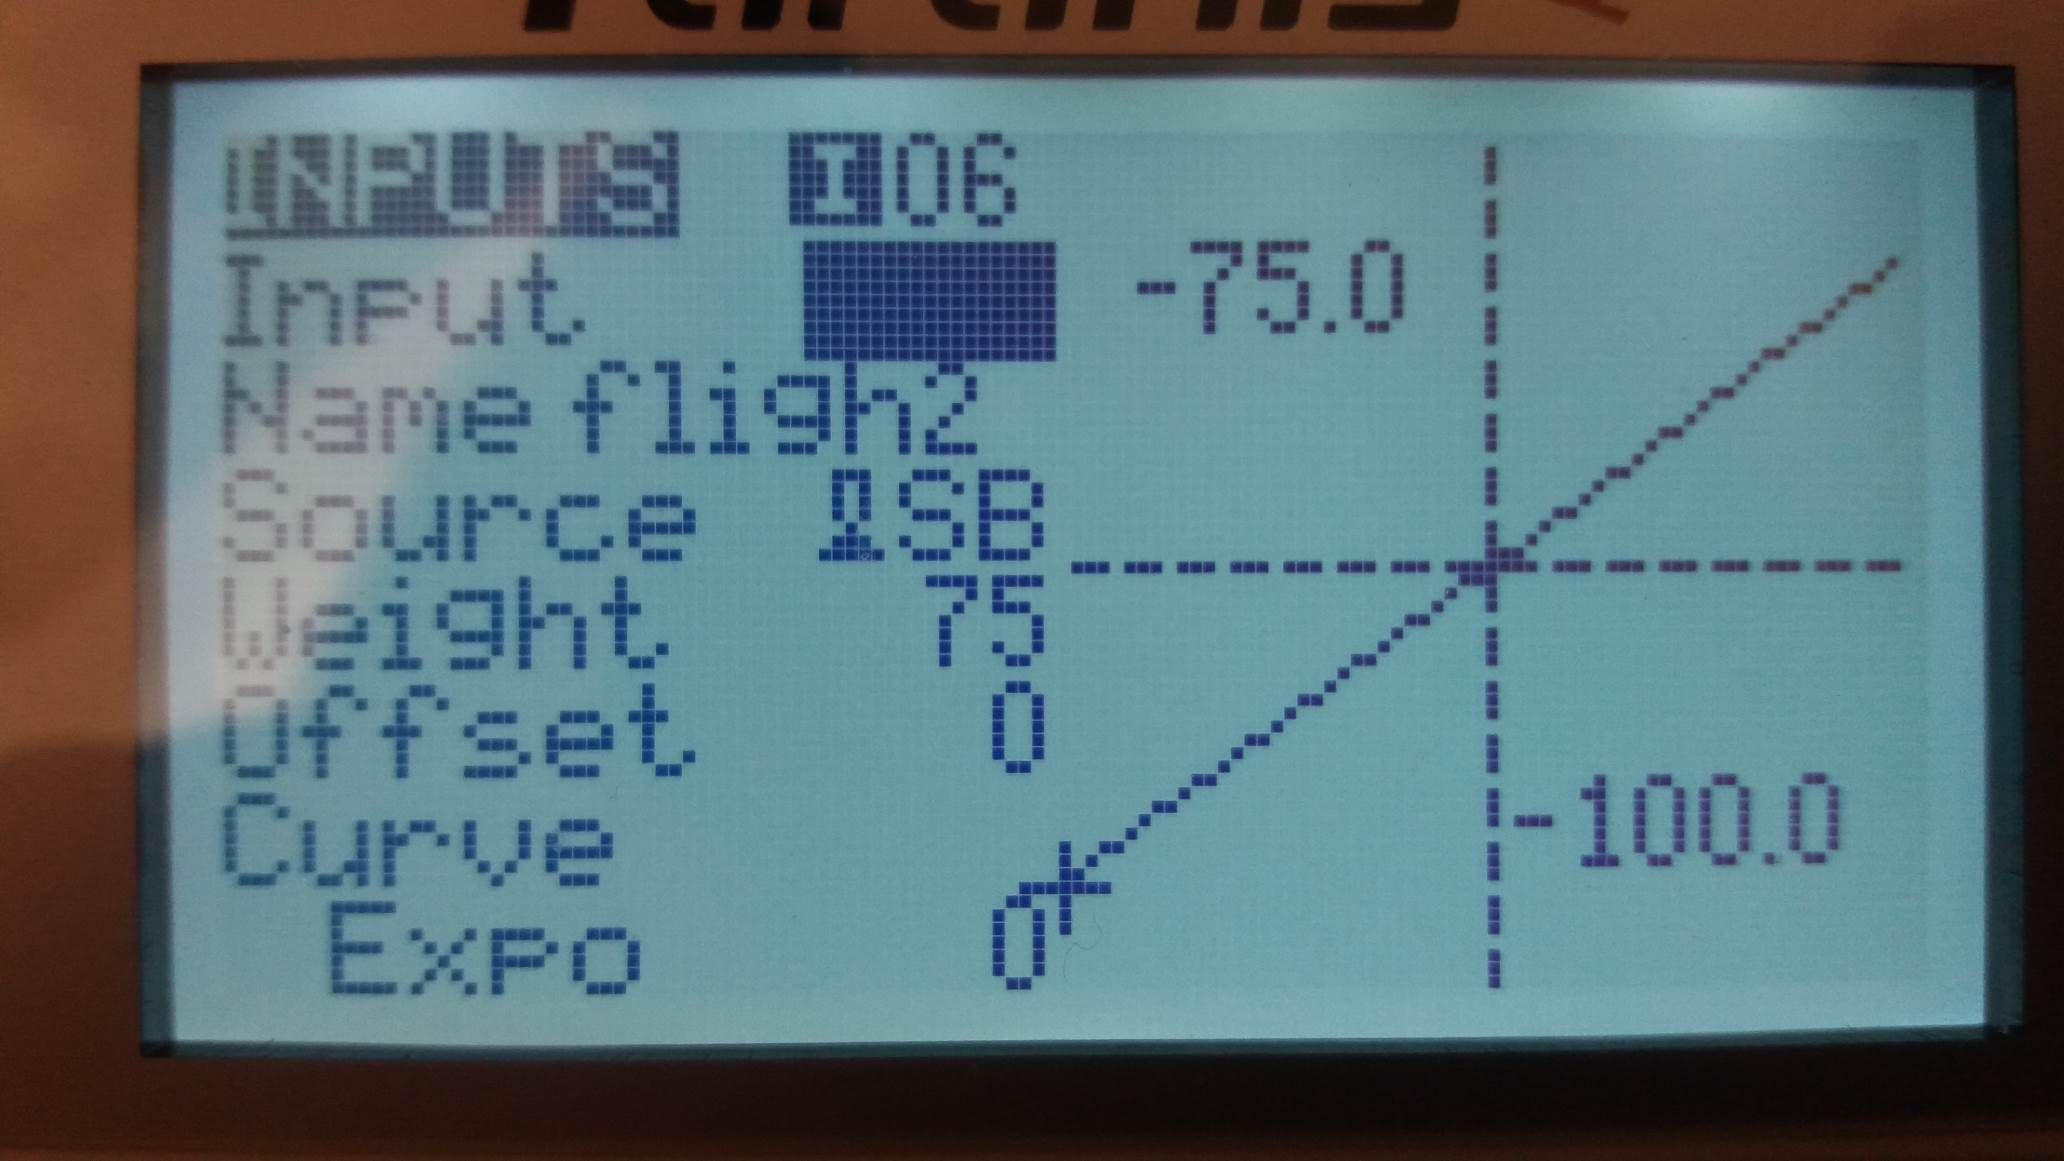
\includegraphics[scale=0.13]{images/lcd/flight_mode_but_2.jpg}
\caption{Linearised flight mode switch 2 input}
\label{fig:taranis_fm_but2}
\end{subfigure}
\begin{subfigure}{0.5\textwidth}
\centering
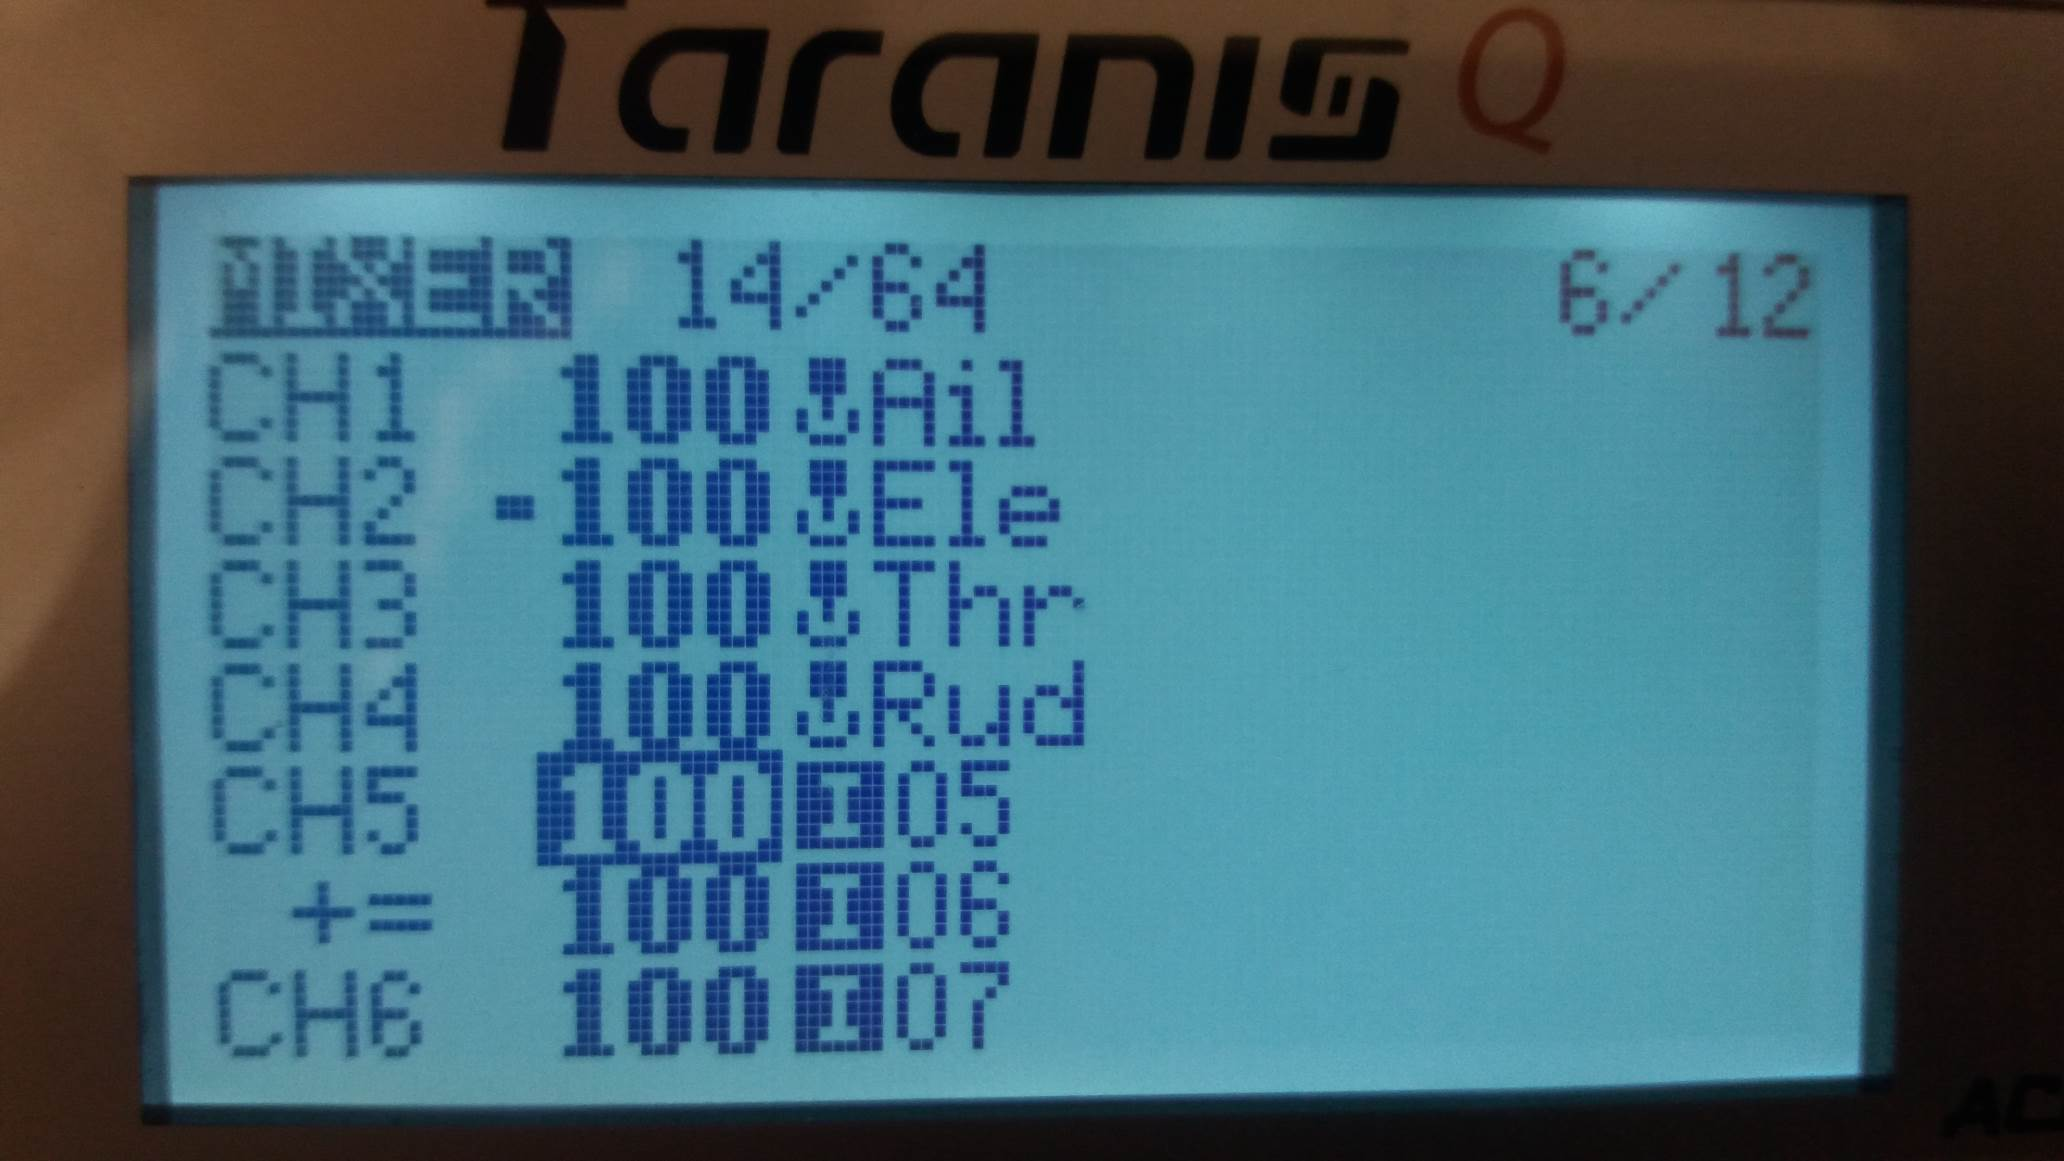
\includegraphics[scale=0.13]{images/lcd/mixer.jpg}
\caption{Mixer muxes input channels to output}
\label{fig:taranis_mux}
\end{subfigure}
\begin{subfigure}{0.5\textwidth}
\centering
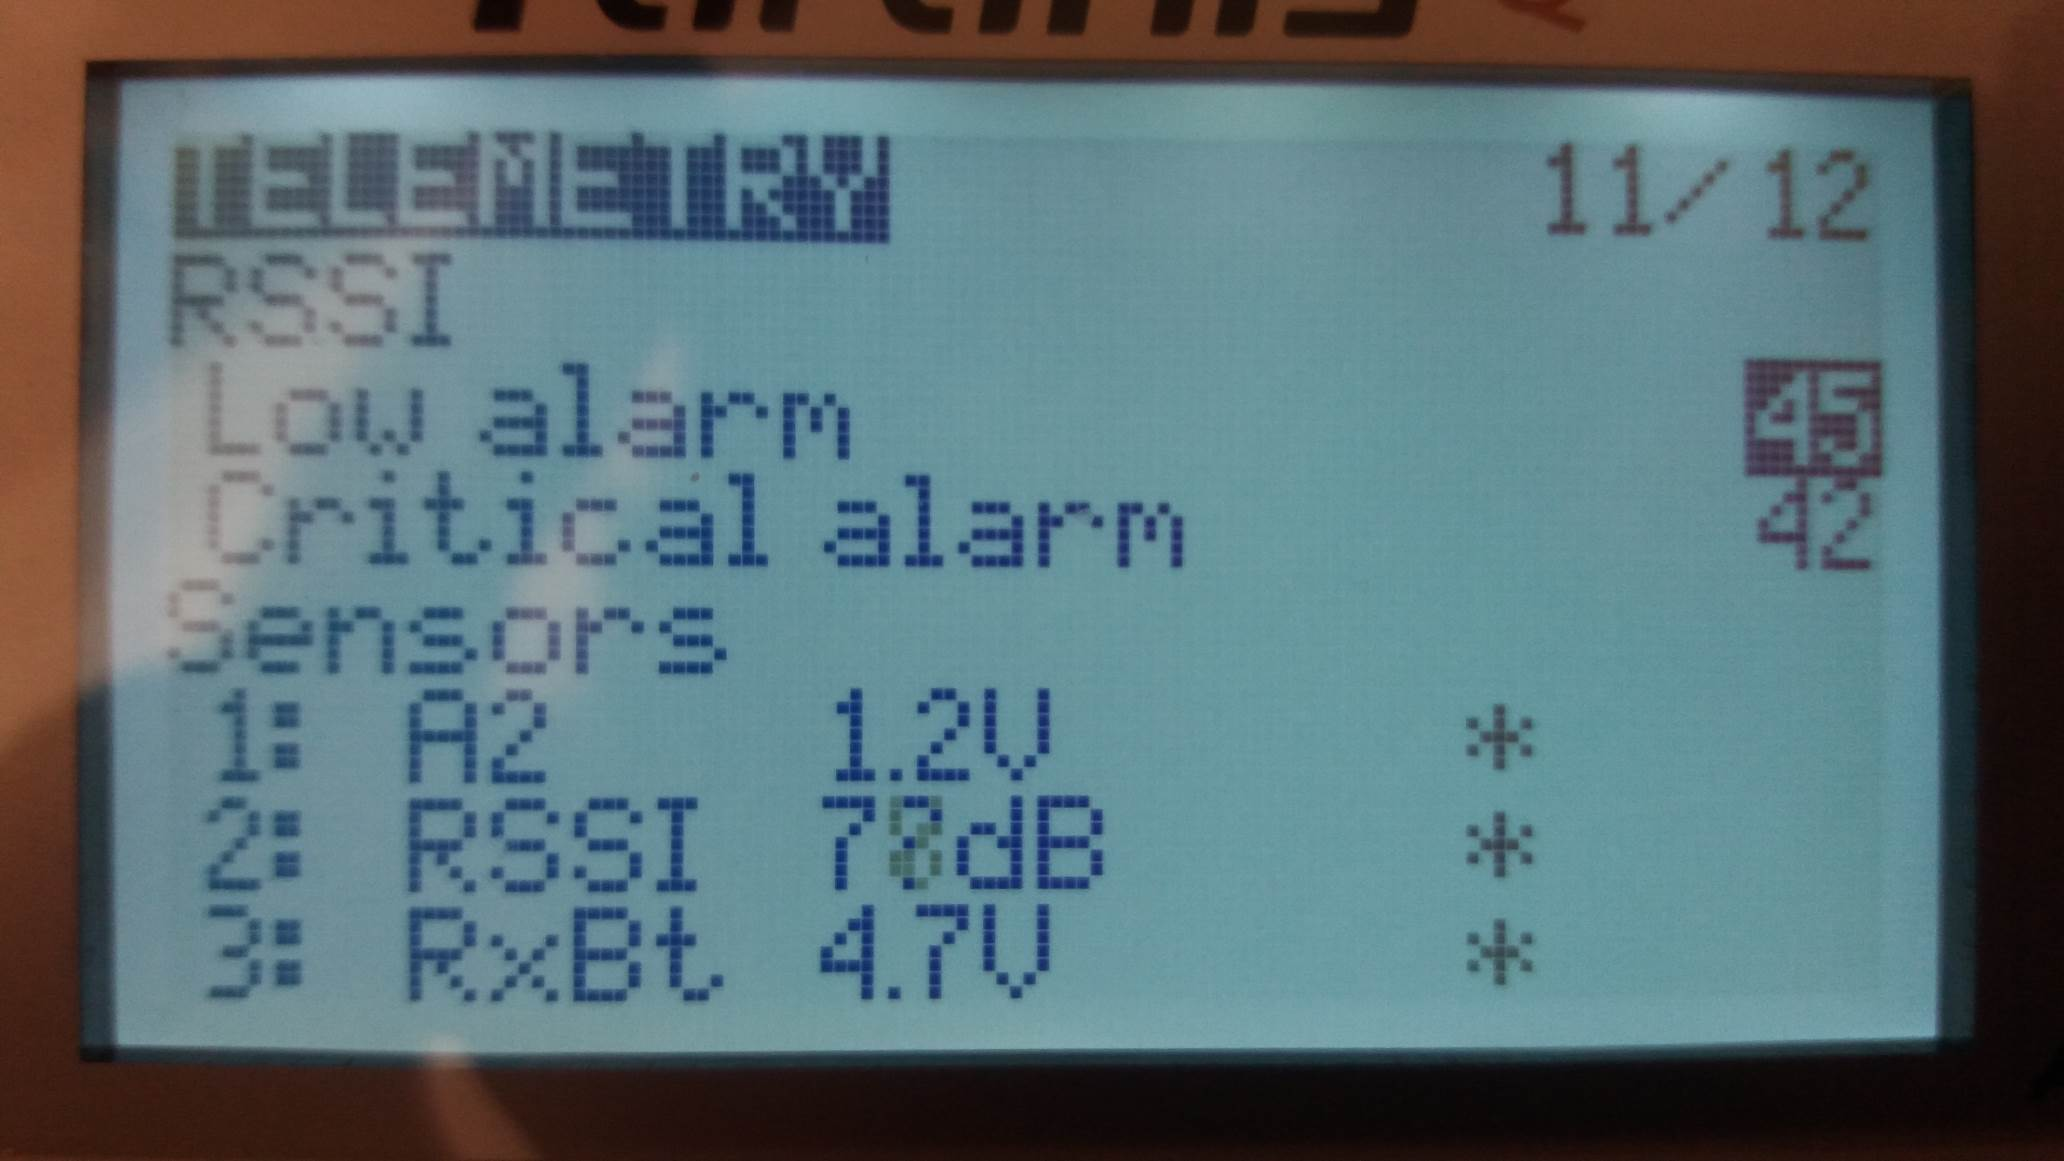
\includegraphics[scale=0.13]{images/lcd/telemetry.jpg}
\caption{Remote sensor feedback}
\label{fig:taranis_telemetry}
\end{subfigure}
\caption{Some important settings for the remote controller}
\label{fig:taranis_lcd}
\end{figure}

The two 3-way flight mode input switches as indicated in Figure \ref{fig:taranis_arm} are multiplexed into channel 5 as in Figure \ref{fig:taranis_mux}. As indicated in Figure \ref{fig:taranis_fm_but1} and \ref{fig:taranis_fm_but2}, the two switches required a peculiar linearisation such that when they are multiplexed, there exist 6 PWM positions within the duty cycle range. \begin{equation}PWM\ flight\ mode\ output\ values\ \in [1165, 1295, 1425, 1555, 1685, 1815]\ ms\end{equation}
This allows the PWM outputs to exist within the ranges as indicated in Figure \ref{fig:flight_modes}.

\begin{figure}[H]
\centering
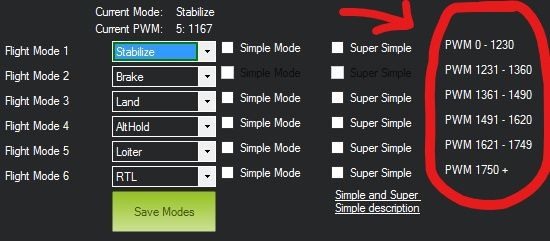
\includegraphics[scale=0.5]{images/flight_modes.JPG}
\caption{Flight modes}
\label{fig:flight_modes}
\end{figure}

To arm the drone for takeoff, move the left controller stick to the bottom right for 2 seconds, as in Figure \ref{fig:taranis_arm}. Also, lift the safety `Cut motors' switch.

\begin{figure}[H]
\centering
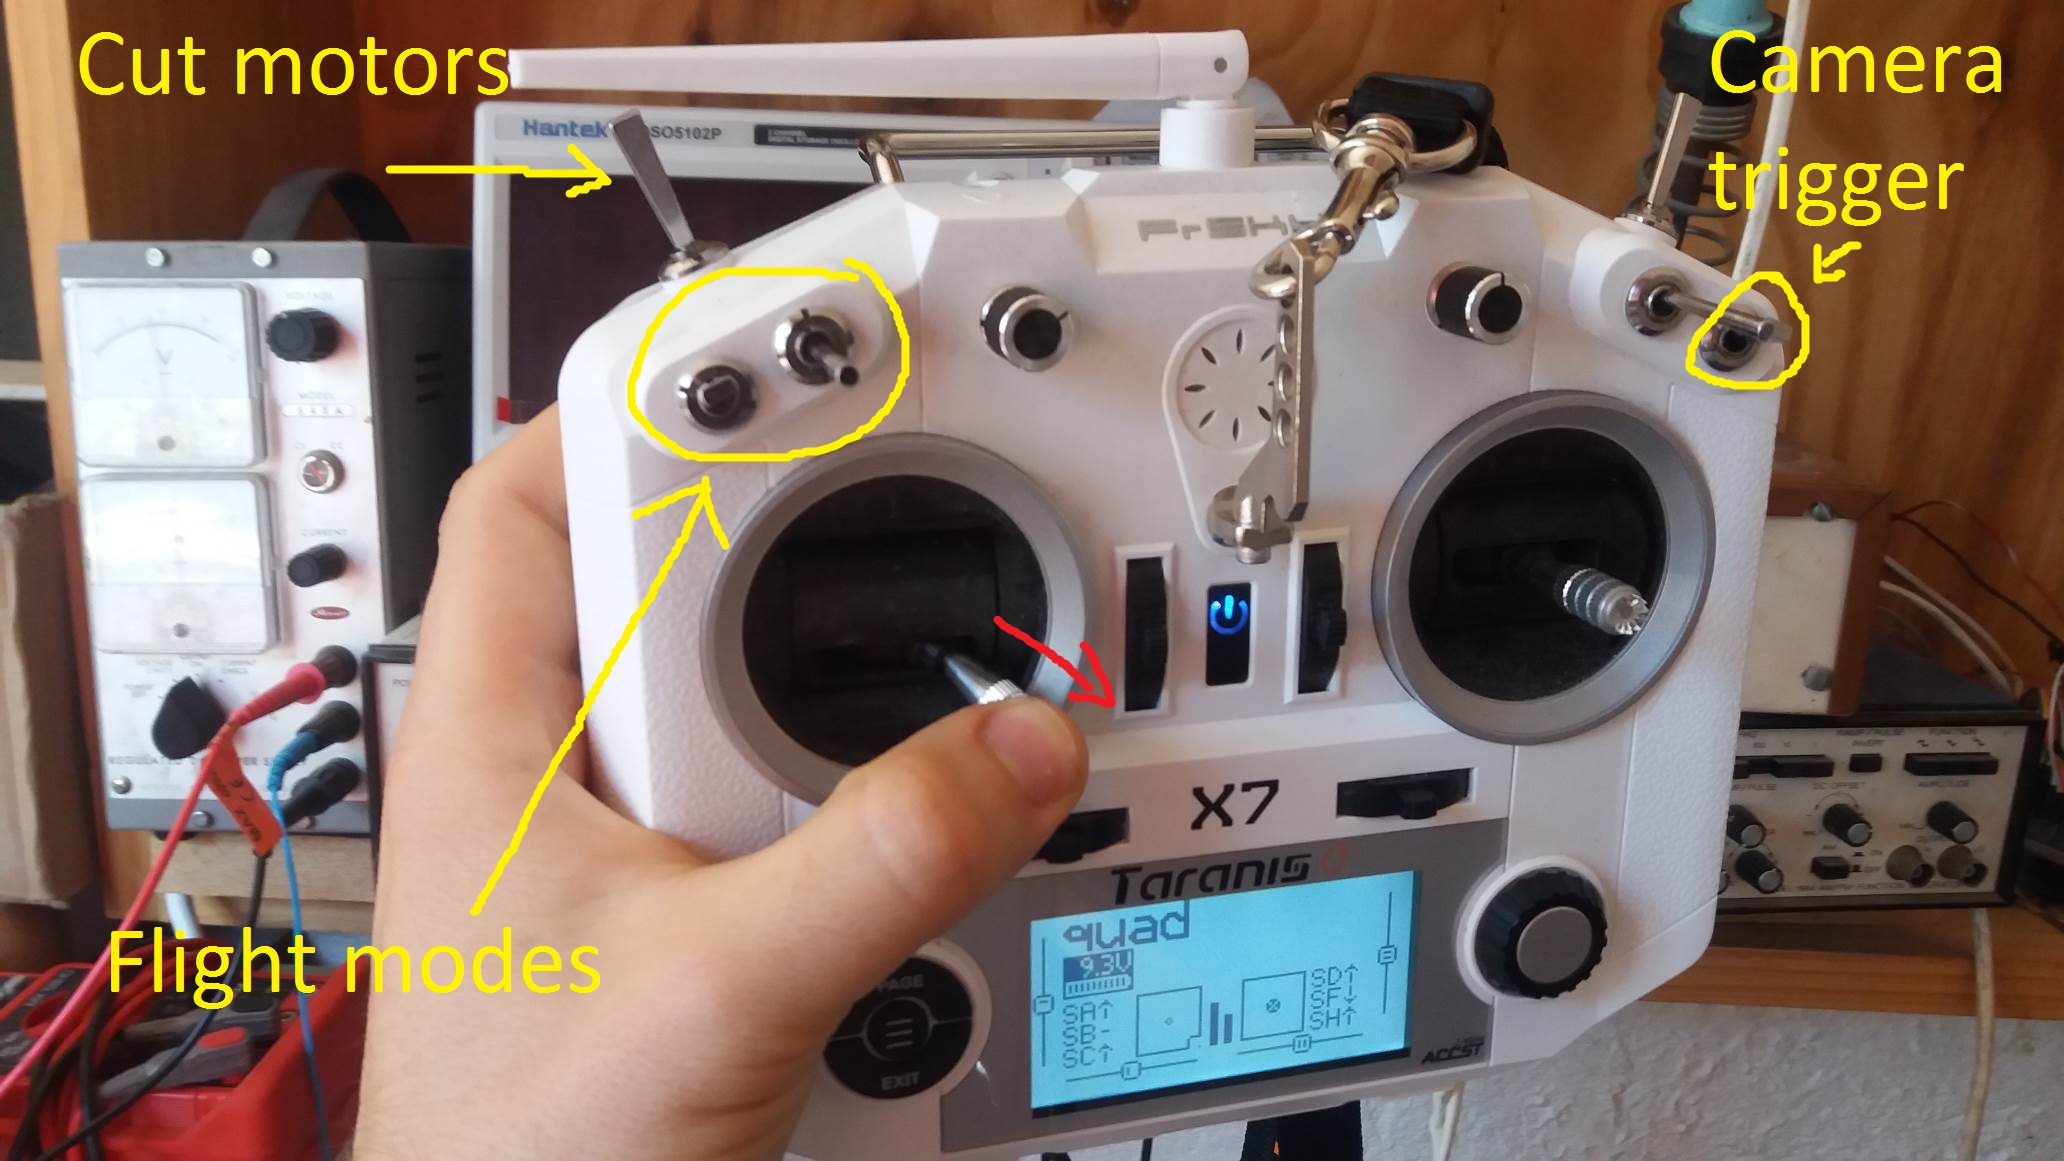
\includegraphics[scale=0.17]{images/taranis_arm.jpg}
\caption{Arming the drone (red arrow)}
\label{fig:taranis_arm}
\end{figure}

\section{Software}

This will be handled by two Raspberry Pis. Both will be used to take photos through each of their single CSI ports. The Raspberry Pis will communicate with each other via direct ethernet connection. Twisted-pair is not necessary since the driver automatically swaps the RX and TX lines.\\

Initially, one Raspberry Pi was to be used with a camera multiplexer as in Section \ref{sec:simultaneous_trig}, but it didn't work, and therefore two raspberry pis were used. Just as well, as the flight controller uses all but 1 GPIO pin.\\

A real-time kernel will be used for the Ardupilot Firmware used on the `flight controller' Raspberry Pi, extended by a Navio2. \\

\section{Testing}

There was a case where one foot holding vibration dampeners broke and induced an unstable asynchronous frequency when rolling in a certain direction as in Figure \ref{fig:leafy}.

\begin{figure}[H]
\centering
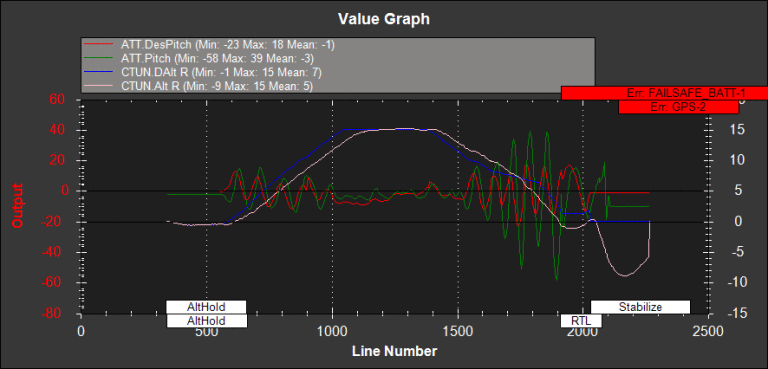
\includegraphics[scale=0.58]{images/pitch_alt.png}
\caption{Oscillations in pitch and roll}
\label{fig:leafy}
\end{figure}

The PID values for pitch and roll rate were lowered by about 11\% to account for the frame size as in Figure \ref{fig:tuning}.\\

\begin{figure}[H]
\centering
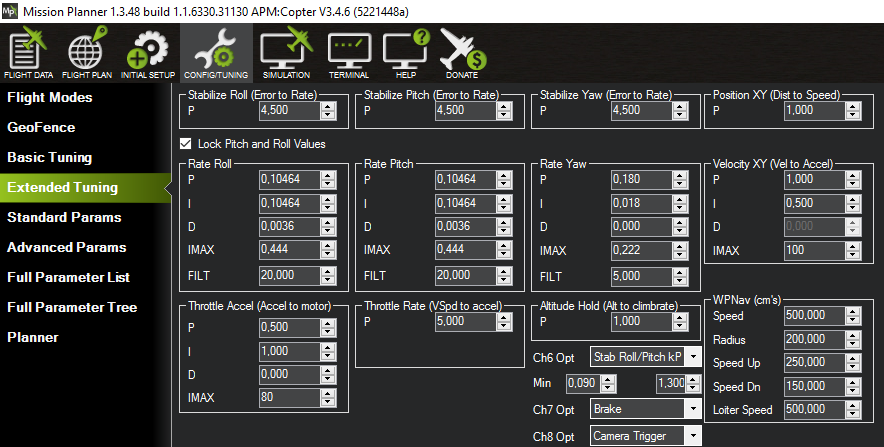
\includegraphics[scale=0.5]{images/tuning.PNG}
\caption{Tuning PID values}
\label{fig:tuning}
\end{figure}

%Relevant flight log data.\\

An RTL2832U software defined radio (SDR) with a receive sensitivity of -140dBm was used to test the range of the 433 MHz transceivers.

\begin{figure}[H]
\begin{subfigure}{0.5\textwidth}
\centering
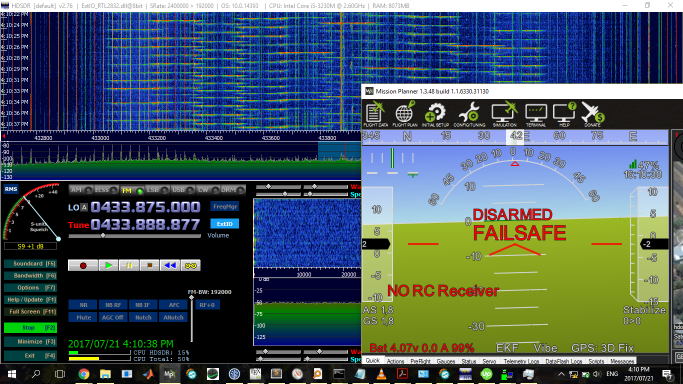
\includegraphics[scale=0.45]{images/range_test.PNG}
\caption{FHSS channel hopping}
\label{fig:range_test}
\end{subfigure}
\begin{subfigure}{0.5\textwidth}
\centering
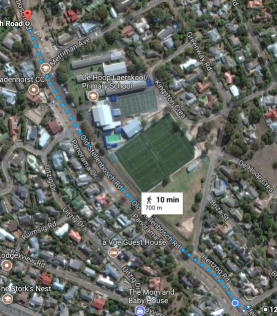
\includegraphics[scale=0.8]{images/range_test_700m.PNG}
\caption{700m NLOS before lost signal}
\label{fig:range_test_700m}
\end{subfigure}
\caption{Range testing}
\label{fig:range}
\end{figure}

Also, compass interference was measured against current draw as in Figure \ref{fig:interference} to lower the chance of errors.

\begin{figure}[H]
\centering
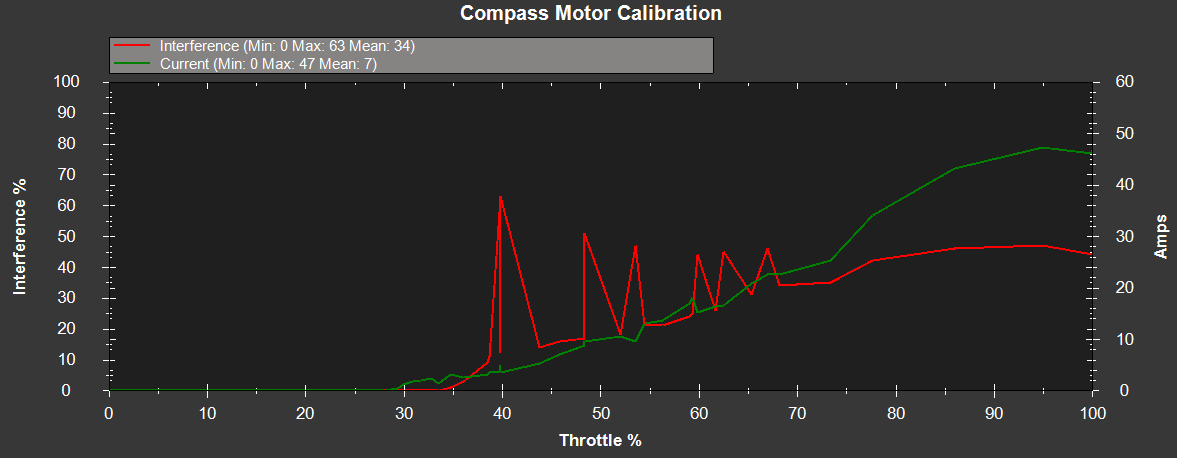
\includegraphics[scale=0.35]{images/comp_mot_true_current.PNG}
\caption{Measuring compass interference vs current draw.}
\label{fig:interference}
\end{figure}


%Many other tests were performed on each component subsystem. For example, a current meter was used to verify the current constants for both power modules, and 
\chapter{Image Acquisition and Calibration}

As mentioned in the system architecture, images need to be taken simultaneously. There also needs to be two cameras due to the way the cameras are constructed, with a Bayer matrix (See intrinsic parameters) for each pixel. At the time of inception, one could only isolate NIR from RGB using separate cameras. Attempts to have both on a single camera were ineffective (explain why).\\

\noindent
The

\section{Review of concepts}

These concepts are crucial to understand the reasoning behind certain decisions.

\subsection{Intrinsic Parameters}

focal length

\subsection{Distortion}

(picture of distortion)

\subsubsection{Bayer matrix}

\subsection{Extrinsic Parameters}

translation, rotation, sun, glare

\subsection{Camera Calibration}

(picture of undistortion).

\subsubsection{Jello effect}

ripple

\section{Filters}

The blue Rosco 2008 filter is used as in Figure \ref{fig:blue_filter}, and passes only NIR within the green and red channels, as shown in Figure \ref{fig:blue_curve}.

\begin{figure}[H]
\begin{subfigure}{0.5\textwidth}
\centering
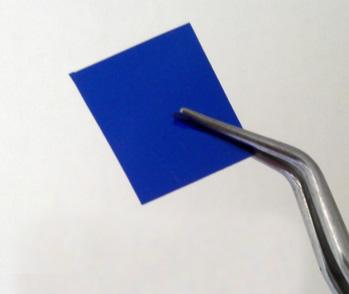
\includegraphics[scale=0.45]{images/blue_filter.jpg}
\caption{Blue Rosco 2008 filter \cite{blue_filter}}
\label{fig:blue_filter}
\end{subfigure}
\begin{subfigure}{0.5\textwidth}
\centering
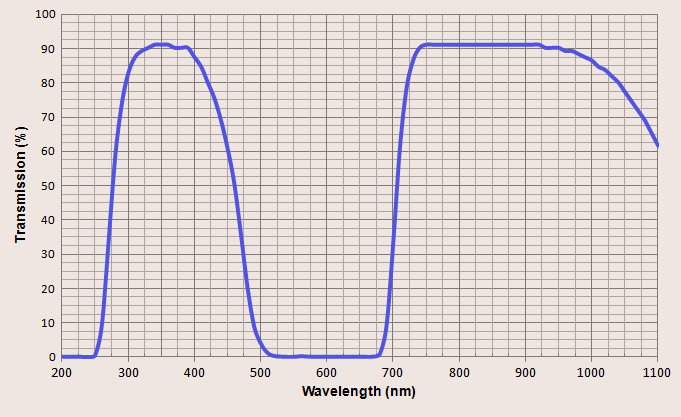
\includegraphics[scale=0.42]{images/superblueinfraredfiltercurve.png}
\caption{Blue filter transmission curve.}
\label{fig:blue_curve}
\end{subfigure}
\caption{Blue filter characteristics \cite{blue_curve}}
\label{fig:blue_character}
\end{figure}

\section{Camera mount}

Ripple / jello

Thus, a DC brushless motorised gimbal will not be necessary.

\section{Simultaneous triggering}

Initially TCP triggering was used, but the overhead and asynchronous nature meant that it was never consistently triggered at the same time. Instead, the clocks are sychronised using NTP, and attempt to trigger every second, on the second. The latter solution works quite well, with an occassional few milliseconds difference in stereo captures.

\section{Calibration}

\subsection{Calibration Technique}

\subsection{Measured Results}

\section{Stereo-rectification}

\subsection{Measured Results}
\chapter{Image Processing and NDVI}
\label{sec:image_processing}
%SIFT, mapping, geotagging, alignment,\\

Once the images are undistorted as in Section \ref{sec:undistortion}, the images can be aligned using stereo-correspondence before an NDVI is performed.\\

A scale-invariant-feature-transform is applied to the images to align them using an affine transform. An NDVI calculation is applied to the matched images, with a floating point output image. A LUT colourmap is applied to visibly distinguish different areas and their meanings in the final image.

\section{Feature Detection}

There are different types of feature detection. 
\begin{itemize}
	\item Harris Corner Detection
	\item Shi-Tomasi Corner Detection
	\item SIFT (Scale-Invariant Feature Transform)
	\item SURF (Speeded-Up Robust Features)
	\item FAST (Features from Accelerated Segment Test)
	\item BRIEF (Binary Robust Independent Elementary Features)
	\item ORB (Oriented FAST and Rotated BRIEF)
%	\item BRISK, FREAK, KAZE, and AKAZE
\end{itemize}

There are also different types of feature matching.

\begin{itemize}
	\item Feature Matching + Homography to find Objects
	\item FLANN (Fast Library for Approximate Nearest Neighbors) based matcher
\end{itemize}

Harris Corner detection is useful for the chessboard calibration technique as in Section \ref{sec:cal_technique}. Shi-Tomasi improved the scoring function of Harris, but it is more appropriate for tracking. SIFT provides keypoints and descriptors. It also does not depend on the scale of a corner, unlike in Figure \ref{fig:sift_scale}. SURF is good at dealing with blurring and rotation, but not at handling viewpoint and illumination change as in SURF. FAST is better from a realtime, limited resource application point of view. Although it is several times faster than the other detectors, it is not robust against high levels of noise, and depends on a threshold. BRIEF is a quicker feature descriptor with lower memory usage, but feature detection such as SIFT, SURF is still needed. ORB is a good alternative to SIFT and SURF in performance, and is not patented.\\

\begin{figure}[H]
\centering
\includegraphics[scale=0.5]{images/sift_scale_invariant.jpg}
\caption{Harris corner detection on scaled corners. \cite{calib3d}}
\label{fig:sift_scale}
\end{figure}

\subsection{Feature matching}

SIFT returns landmark correspondence points between the stereo images.\\

It will then use brute-force feature matching, which calculates for each descriptor in the first image, the distance between it and all the features in the second image, returning the closest one. If the second closest corresponding point is within a threshold normalized distance of 0.8, according to David G. Lowe, it is discarded. The remaining candidates are filtered by geometric consensus.\\

%SURF is faster than SIFT, since it approximates the Laplacian of Gaussian with Box Filter instead of Difference of Gaussian.

\subsection{Homography}

Once the corresponding features are found, an affine transform matrix is found. For example, the estimated transformation matrix may be as in Equation \ref{eq:affine}.

\begin{equation}\label{eq:affine}
1.29837\cdot\begin{bmatrix}3 &3\end{bmatrix}
\begin{bmatrix}
1.00123 & 0.00442 & -10.778 \\ 0.11146\cdot10^-3 & 1.00130 & 19.372
\end{bmatrix}
\end{equation}

\section{Stitching and mapping}

A few images are stitched together to show proof-of-concept as in Figure \ref{fig:stitch_map}. A subset of about 100 images total are processed using MME \cite{mme}.

\begin{figure}[H]
\begin{subfigure}{0.5\textwidth}
\centering
\includegraphics[scale=0.35]{images/map_rgb.png}
\caption{RGB map}
\end{subfigure}
\begin{subfigure}{0.5\textwidth}
\centering
\includegraphics[scale=0.4]{images/map_ir.png}
\caption{NIR map}
\end{subfigure}
\caption{Maps processed using MME}
\label{fig:maps}
\end{figure}

The images are then co-registered using an algorithm called bUnwarpJ \cite{bunwarpj} as in Figure \ref{fig:stitch_map}. Image registration is based on elastic deformations represented by B-splines and pyramid coefficients. 

\begin{figure}[H]
\centering
\includegraphics[scale=0.35]{images/map_ndvi.png}
\caption{NDVI performed using bUnwarpJ}
\label{fig:stitch_map}
\end{figure}

There does exist a larger map in Appendix \ref{app:ndvi_map}.

%\begin{figure}[H]
%\centering
%\includegraphics[scale=0.35]{images/ndvi_stitch_example.jpg}
%\caption{Photos stitched into a map}
%\label{fig:stitch_map}
%\end{figure}

\section{Calibration Plate}
\label{sec:cal_plate}

Moderate NDVI values apply to young/older (senescing) crops or grasslands and shrubs from about 0.2 to 0.5. Higher NDVI values from about 0.6 to 0.9 correspond to dense vegetation such as that found in forests or crops at their peak growth stage. \cite{ndvi_values}\\

NDVI values can drift due to sunlight, clouds, glare etc. The values have a scientific basis, and it would be good to calibrate the equipment before every flight, otherwise one can only retrieve relative NDVI values, which may not be very helpful over a long period of time. In general, the idea is to get consistent results, no matter the time or place.\\

A calibration plate from MicaSense was investigated. It has an NDVI value of 0.18. There is also a piece of red and blue paper, with the hope that it can be used as a cheap calibration plate.

\begin{figure}[H]
\begin{subfigure}{0.5\textwidth}
\centering
\includegraphics[scale=0.15]{images/rgb_cal.jpg}
\caption{RGB image}
\end{subfigure}
\begin{subfigure}{0.5\textwidth}
\centering
\includegraphics[scale=0.15]{images/ndvi_cal.jpg}
\caption{Processed NDVI image}
\end{subfigure}
\caption{Images take from Sony cameras used throughout project}
\label{fig:cal_plate}
\end{figure}

The plate has an NDVI value of -0.006, blue paper has 0.171, and red paper has 0.042.
%0,069
%0.073

\begin{figure}[H]
\begin{subfigure}{0.5\textwidth}
\centering
\includegraphics[scale=0.35]{images/sequoia_redcal.jpg}
\caption{Red (grayscale) image}
\end{subfigure}
\begin{subfigure}{0.5\textwidth}
\centering
\includegraphics[scale=0.35]{images/sequoia_ndvical.jpg}
\caption{Processed NDVI from red and NIR image}
\end{subfigure}
\caption{Images taken from Parrot Sequoia}
\label{fig:cal_plate}
\end{figure}

The plate has an NDVI value of -0.088, blue paper has 0.211, and red paper has 0.085. These values seem about 75\% larger, but it is hard to quantify if it is more sensitive. Both cameras would need to be calibrated to meet the 0.18 NDVI target.\\
%0,06933333333333333333333333333333
%0.128

There does exist radiometric calibration as in Equation \ref{eq:radiometric}, however, it exists outside the scope of the project due to complexity.\\

\begin{equation}\label{eq:radiometric}
L = V(x,y)\ *\ \frac{a_1}{g}*\frac{p\ -\ p_{BL}}{t_e\ +\ a_2y\ -\ a_3t_ey}
\end{equation}

 

Where:\\
$L$ is the spectral radiance in $W/m^2/sr/nm$\\
$p$ is the raw pixel value (normalized)\\
$p_BL$ is the black level value (normalized)\\
$a1,\ a2,\ a3$ are the radiometric calibration coefficients\\
$t_e$ is the image exposure time\\
$g$ is the sensor gain setting\\
$x, y$ is the pixel column and row number\\
$V(x, y)$ is the vignette polynomial function for pixel location $(x, y)$.\\

This is part of the Parrot Sequoia calibration procedure, and it shows that more research needs to be done before the effectiveness of the Sony cameras compared to the Parrot Sequoia can be discussed.
\chapter{System Integration and Testing}

How did everything go together? Drone, cameras, processing. There is a setup period before the system can be used.

quick discussion, issues

testing, + results, + analysis

Capabilities, works well, could be better, compared to this solution. Parrot Sequoia. Quite affordable. Complexity?


% In order for the data to be transmitted successfully, it needs to be in a format acceptable by the GCS. The data will be stored in a JSON packet created using a C++ library\cite{ajson}.

% Code block \ref{code:json1} shows a potential data packet.

% \lstset{language=html,caption={Potential packet},label=code:json1}
% \begin{lstlisting}
% {
%   "temperature": "11.3",
%   "pressure": "99.325"
% }
% \end{lstlisting}

% \begin{figure}
% \centering
% \includegraphics[scale=0.35]{flight_path.png}
% \caption{CanSat flight trajectory\\
% Reproduced from \cite{gopher}}
% \label{fig:flight_path}
% \end{figure}




% \subsection{How to add Tables}

% Use the table and tabular commands for basic tables --- see Table~\ref{tab:widgets}, for example. 

% \begin{table}
% \centering
% \begin{tabular}{l|r}
% Item & Quantity \\\hline
% Widgets & 42 \\
% Gadgets & 13
% \end{tabular}
% \caption{\label{tab:widgets}An example table.}
% \end{table}

% \subsection{How to write Mathematics}

% \LaTeX{} is great at typesetting mathematics. Let $X_1, X_2, \ldots, X_n$ be a sequence of independent and identically distributed random variables with $\text{E}[X_i] = \mu$ and $\text{Var}[X_i] = \sigma^2 < \infty$, and let
% \[S_n = \frac{X_1 + X_2 + \cdots + X_n}{n}
%       = \frac{1}{n}\sum_{i}^{n} X_i\]
% denote their mean. Then as $n$ approaches infinity, the random variables $\sqrt{n}(S_n - \mu)$ converge in distribution to a normal $\mathcal{N}(0, \sigma^2)$.


% \subsection{How to create Sections and Subsections}

% Use section and subsections to organize your document. Simply use the section and subsection buttons in the toolbar to create them, and we'll handle all the formatting and numbering automatically.

% \subsection{How to add Lists}

% You can make lists with automatic numbering \dots

% \begin{enumerate}
% \item Like this,
% \item and like this.
% \end{enumerate}
% \dots or bullet points \dots
% \begin{itemize}
% \item Like this,
% \item and like this.
% \end{itemize}

% \subsection{How to add Citations and a References List}

% You can upload a \verb|.bib| file containing your BibTeX entries, created with JabRef; or import your \href{https://www.overleaf.com/blog/184}{Mendeley}, CiteULike or Zotero library as a \verb|.bib| file. You can then cite entries from it, like this: \cite{greenwade93}. Just remember to specify a bibliography style, as well as the filename of the \verb|.bib|.

% You can find a \href{https://www.overleaf.com/help/97-how-to-include-a-bibliography-using-bibtex}{video tutorial here} to learn more about BibTeX.

% We hope you find Overleaf useful, and please let us know if you have any feedback using the help menu above --- or use the contact form at \url{https://www.overleaf.com/contact}!

\begin{appendices}

\chapter{Bill of Materials}

\begin{itemize}
	\item F450 frame \cite{greenwade93}
	\item Motors \cite{gopher}
\end{itemize}

\end{appendices}

\newpage
\bibliographystyle{plain}
%\bibliographystyle{alpha}
\bibliography{references}

\end{document}